% 4. Versuchsauswertung

\chapter{Auswertung und Diskussion}
\label{chap:versuchsauswertung}

\section{Pfennig}
Begonnen wurde der Versuch mit der Aufnahme einer Kupfermünze, in diese wurden zwei Löcher gebohrt bzw. angebohrt, wobei eines mit einem anderen Material wieder gefüllt worden ist. Mithilfe dieser Probe sollten die Funktion des REM sowie verschiedene Einstellungsmöglichkeiten erkundet werden.\\
Die folgende Abbildung \ref{fig:GsL} zeigt eine Gesamtaufnahme des ''schwarzen'' Lochs.

\begin{figure}[h]
    \centering
    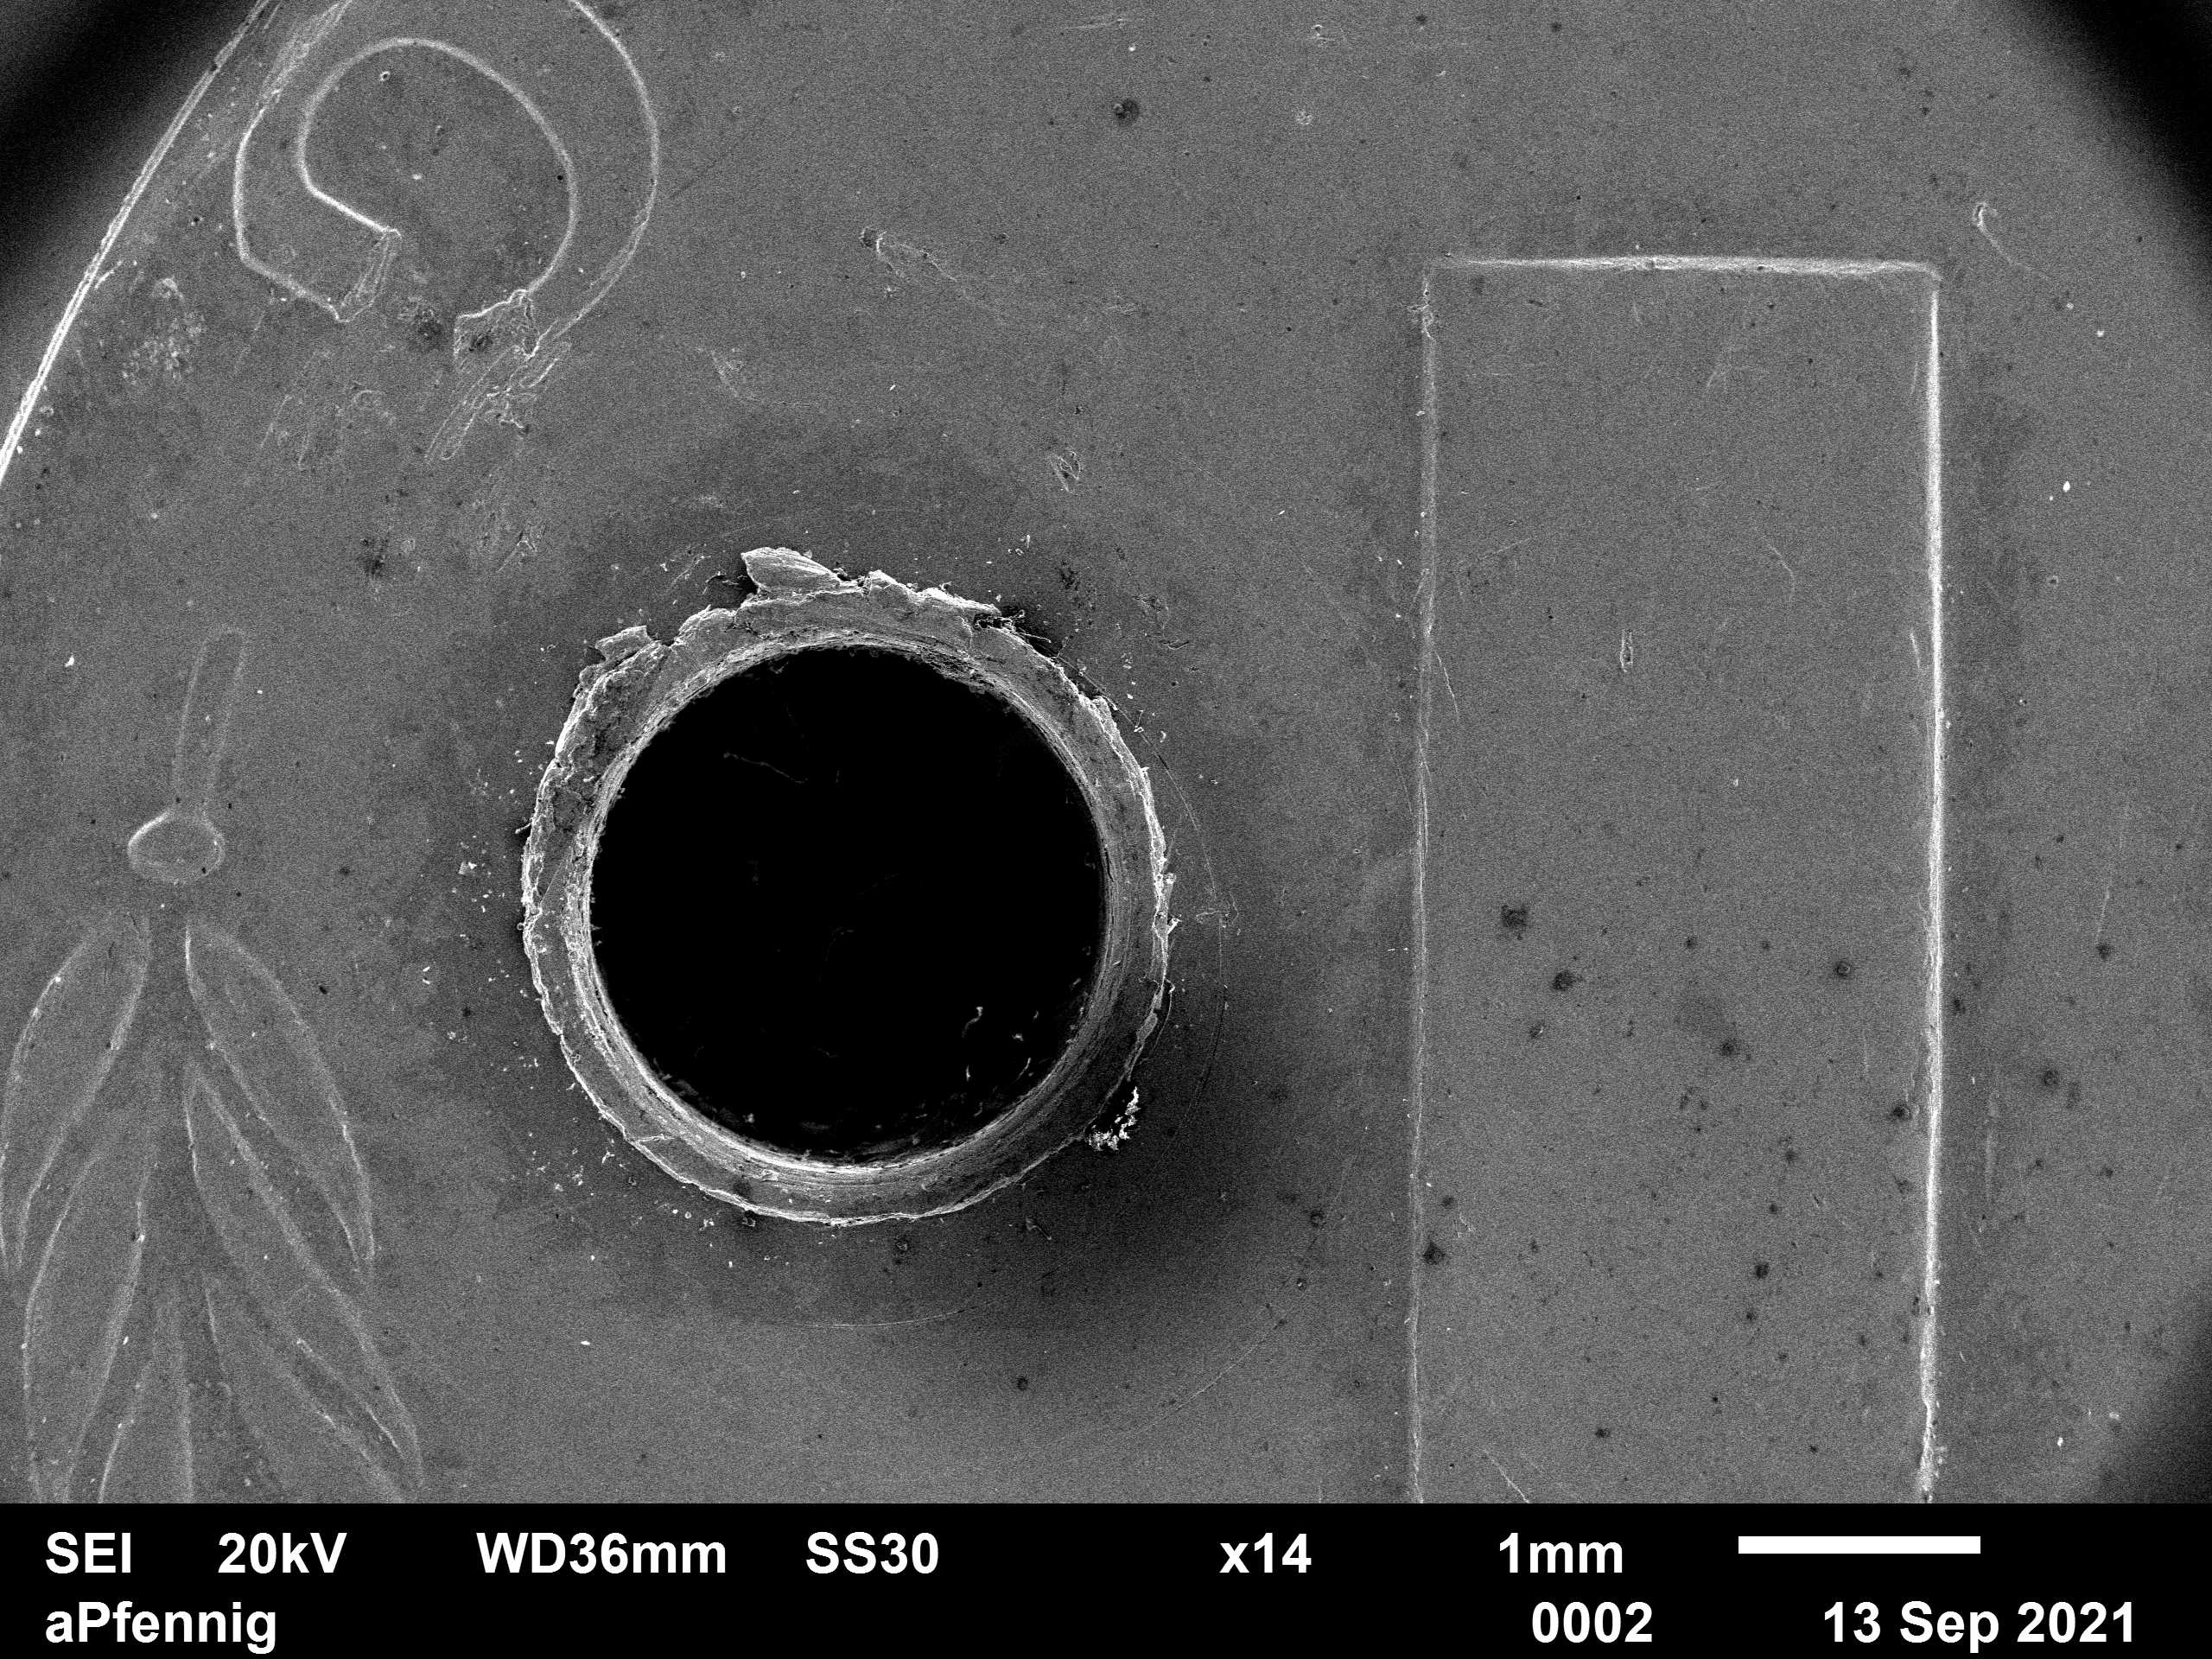
\includegraphics{Auswertung/A/0002.png}
    \caption{Großaufnahme des ''schwarzen'' Lochs}
    \label{fig:GsL}
\end{figure}

\newpage
\subsection*{Aufnahmen bei verschiedenen Parametern}
\label{subsec:Bs}
Als Erstes wurde der Everhart-Thronley-Detektor im SE und RE Modus (SEI) verwendet und dabei die Beschleunigungsspannung variiert.

\begin{figure}[h]
    \centering
    
    \begin{subfigure}[b]{0.45\textwidth}
        \centering
        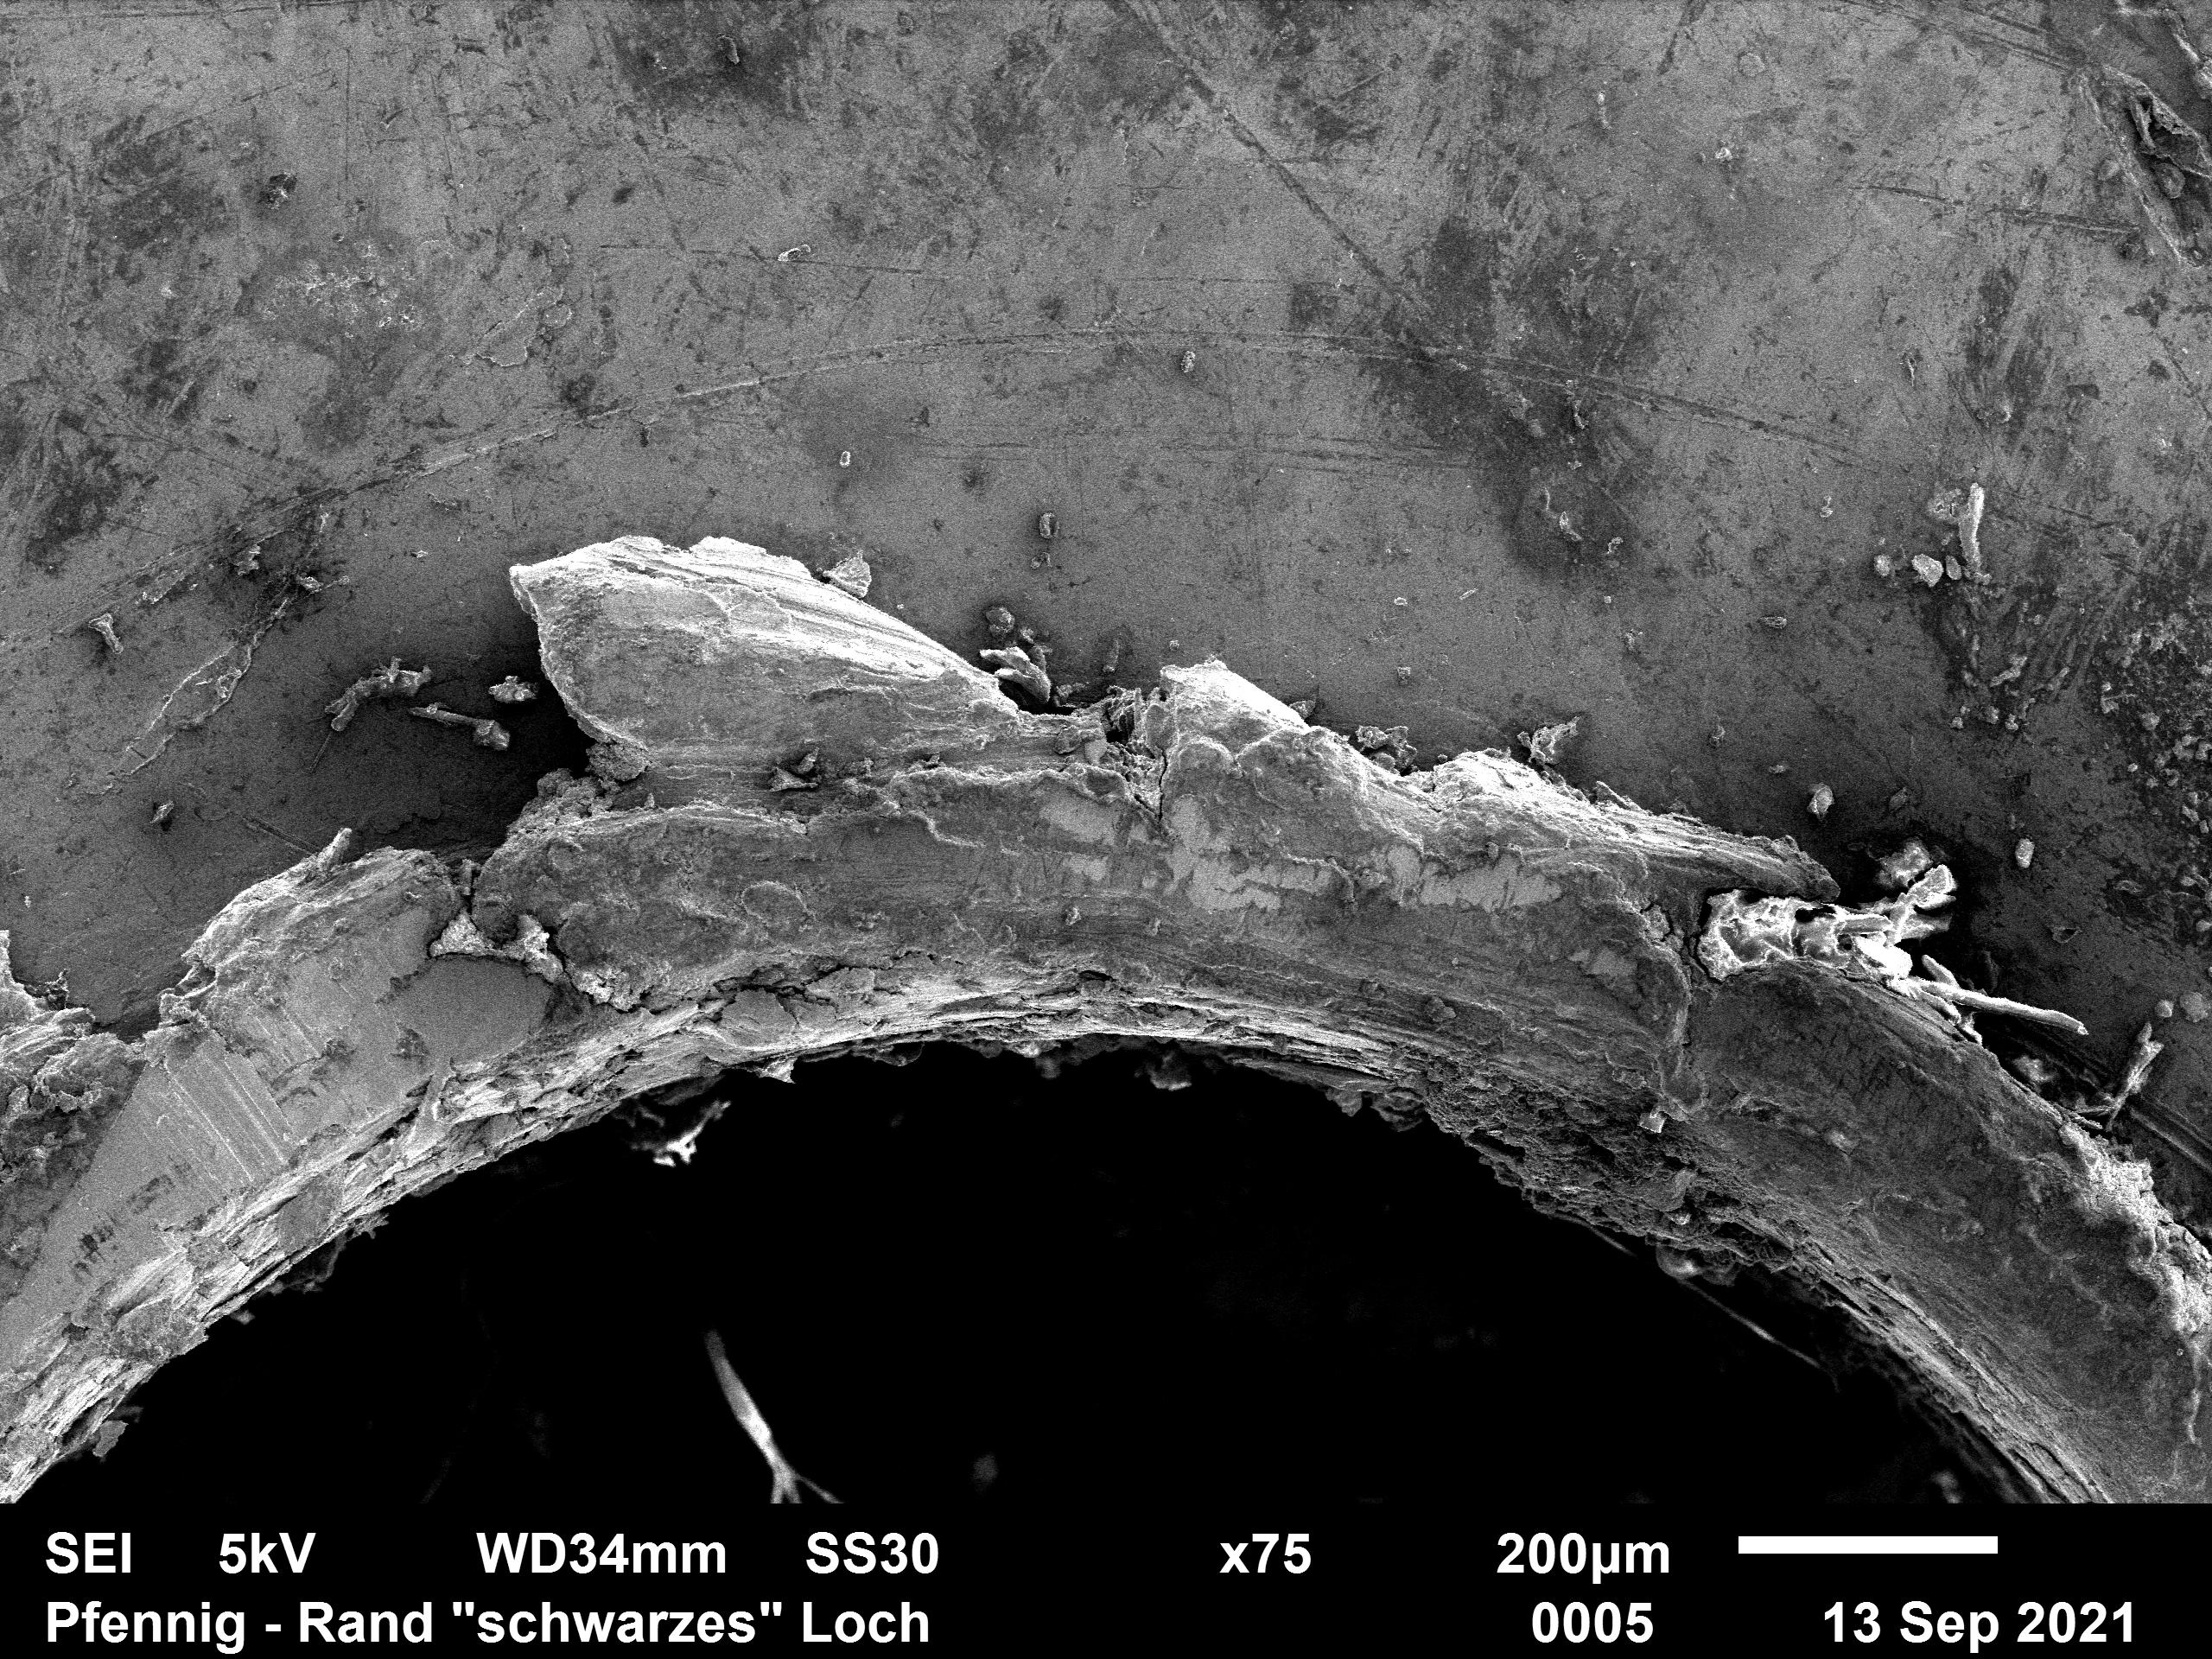
\includegraphics[width=\textwidth]{Auswertung/A/0005.png}
        \caption{$U_B = 5$ kV}
    \end{subfigure}
    \hfill
    \begin{subfigure}[b]{0.45\textwidth}
        \centering
        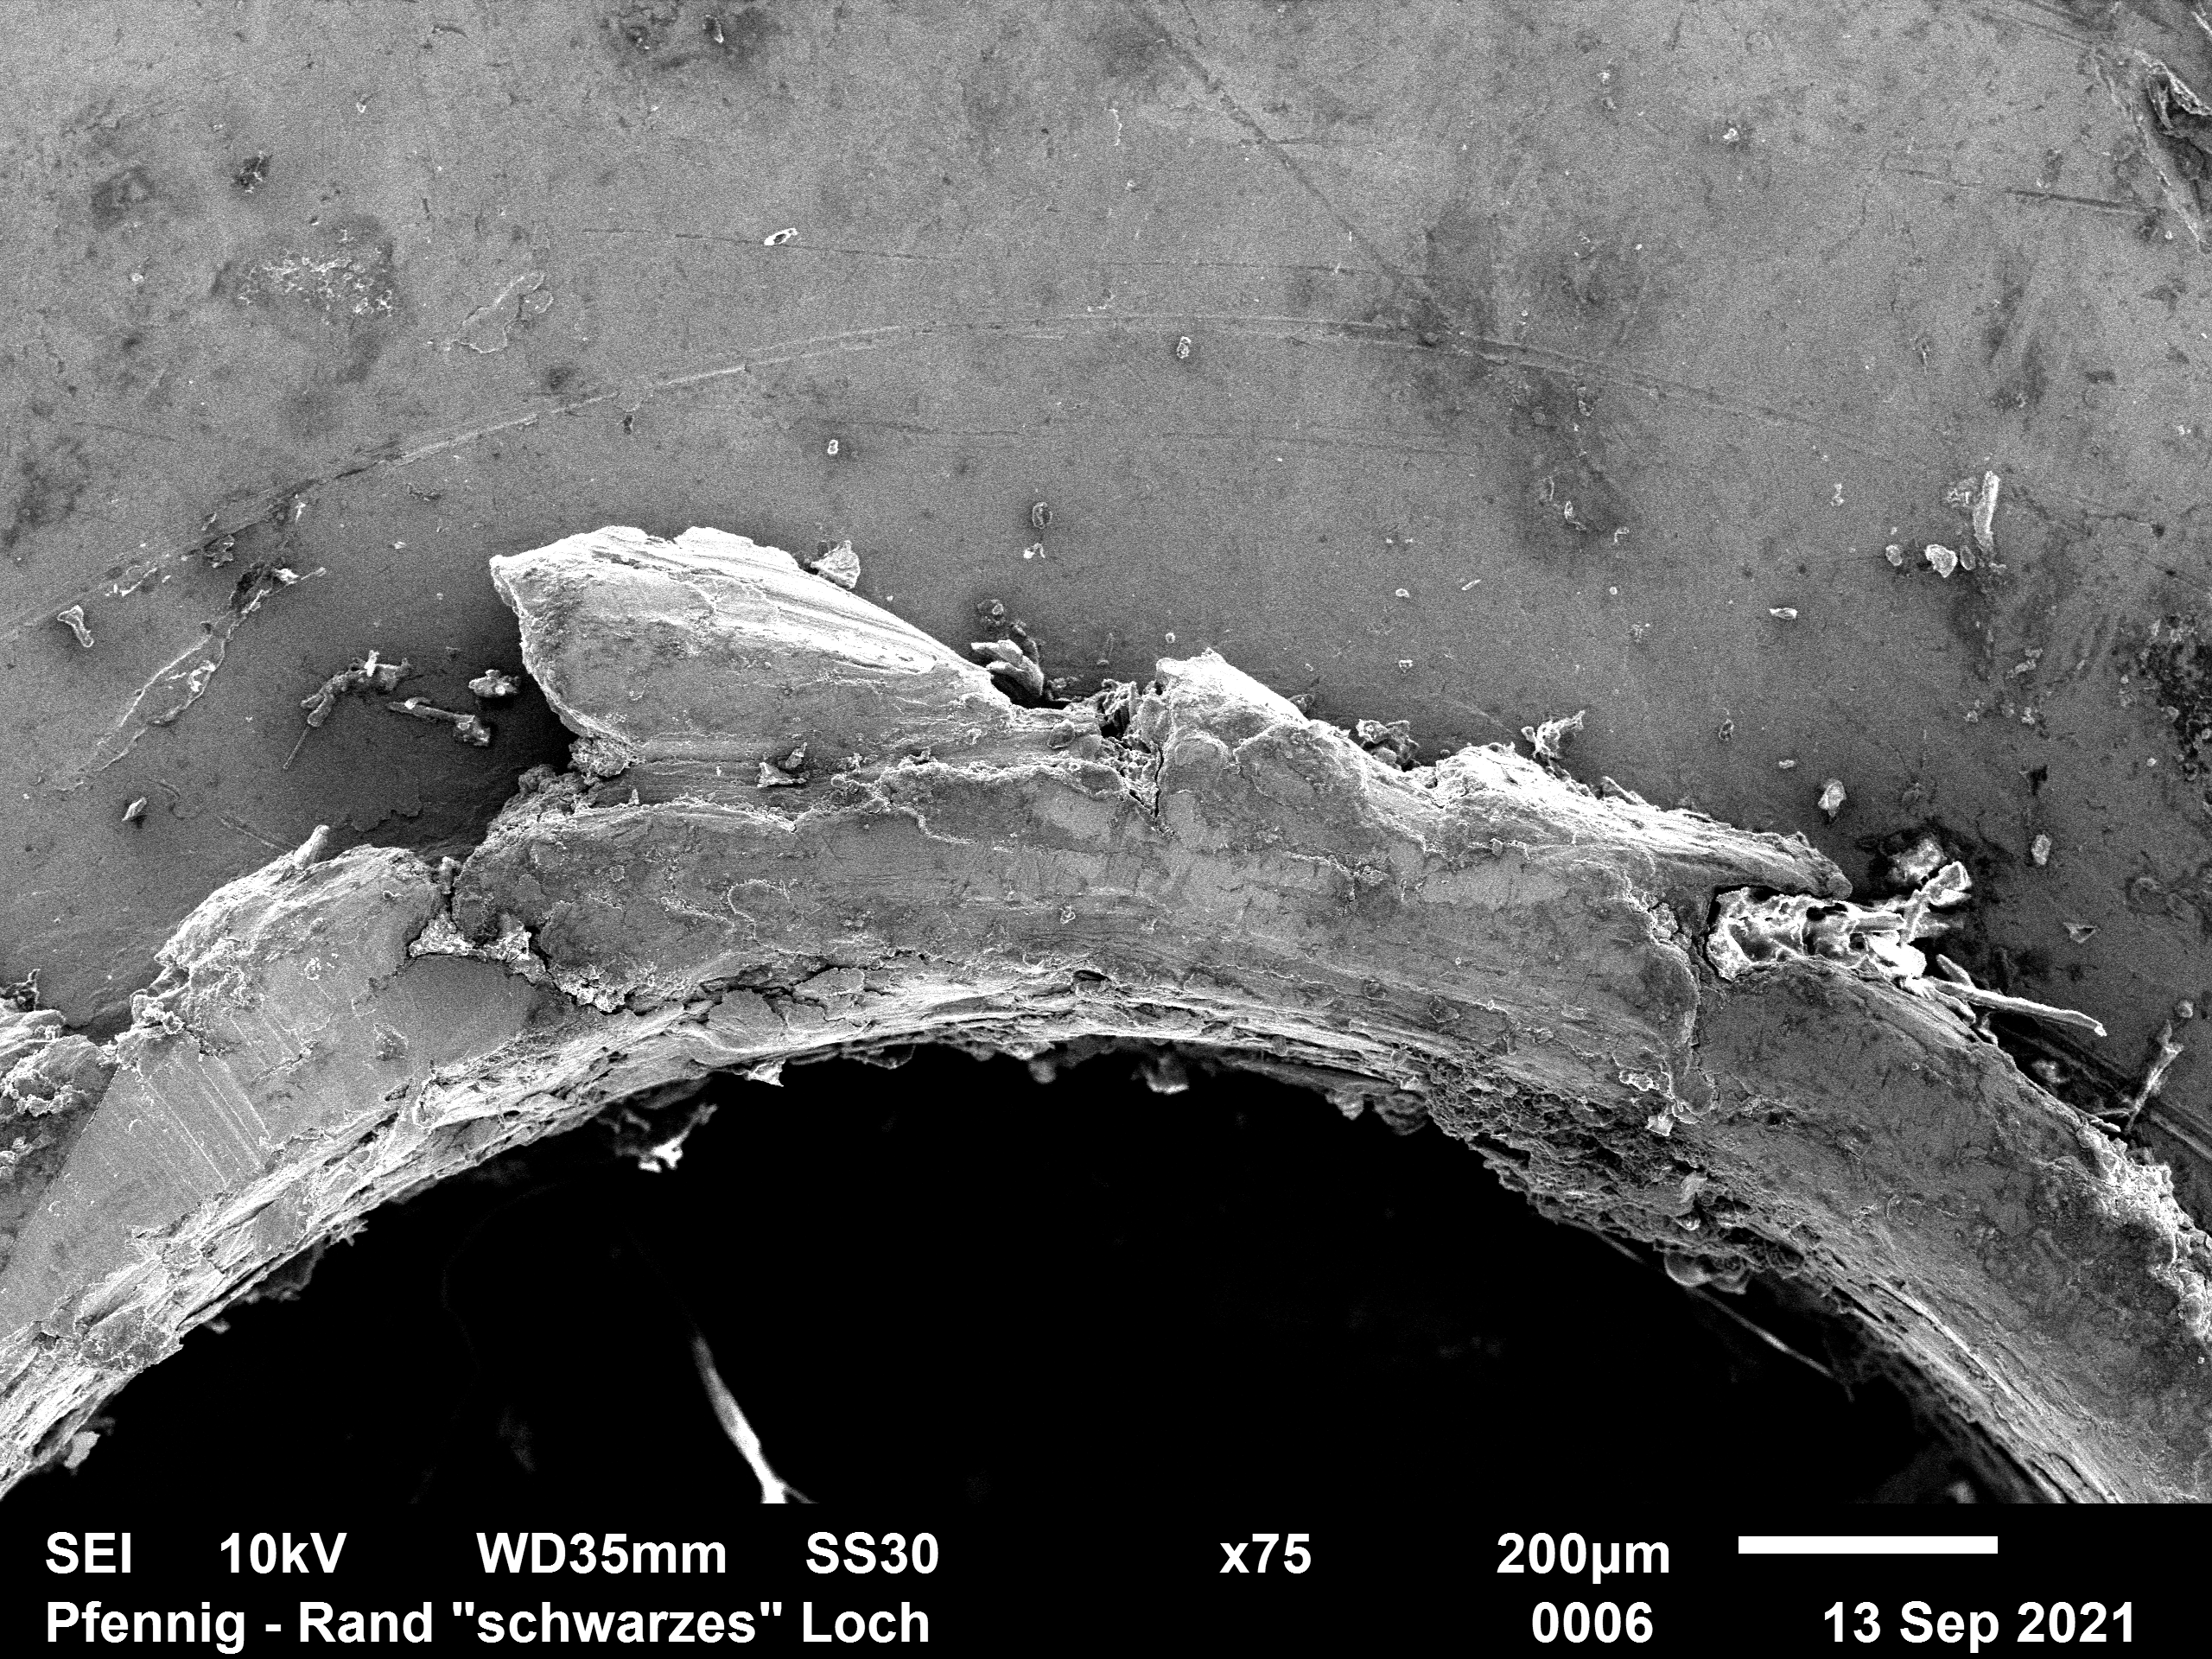
\includegraphics[width=\textwidth]{Auswertung/A/0006.png}
        \caption{$U_B = 10$ kV}
    \end{subfigure}
    \\
    \begin{subfigure}[b]{0.45\textwidth}
        \centering
        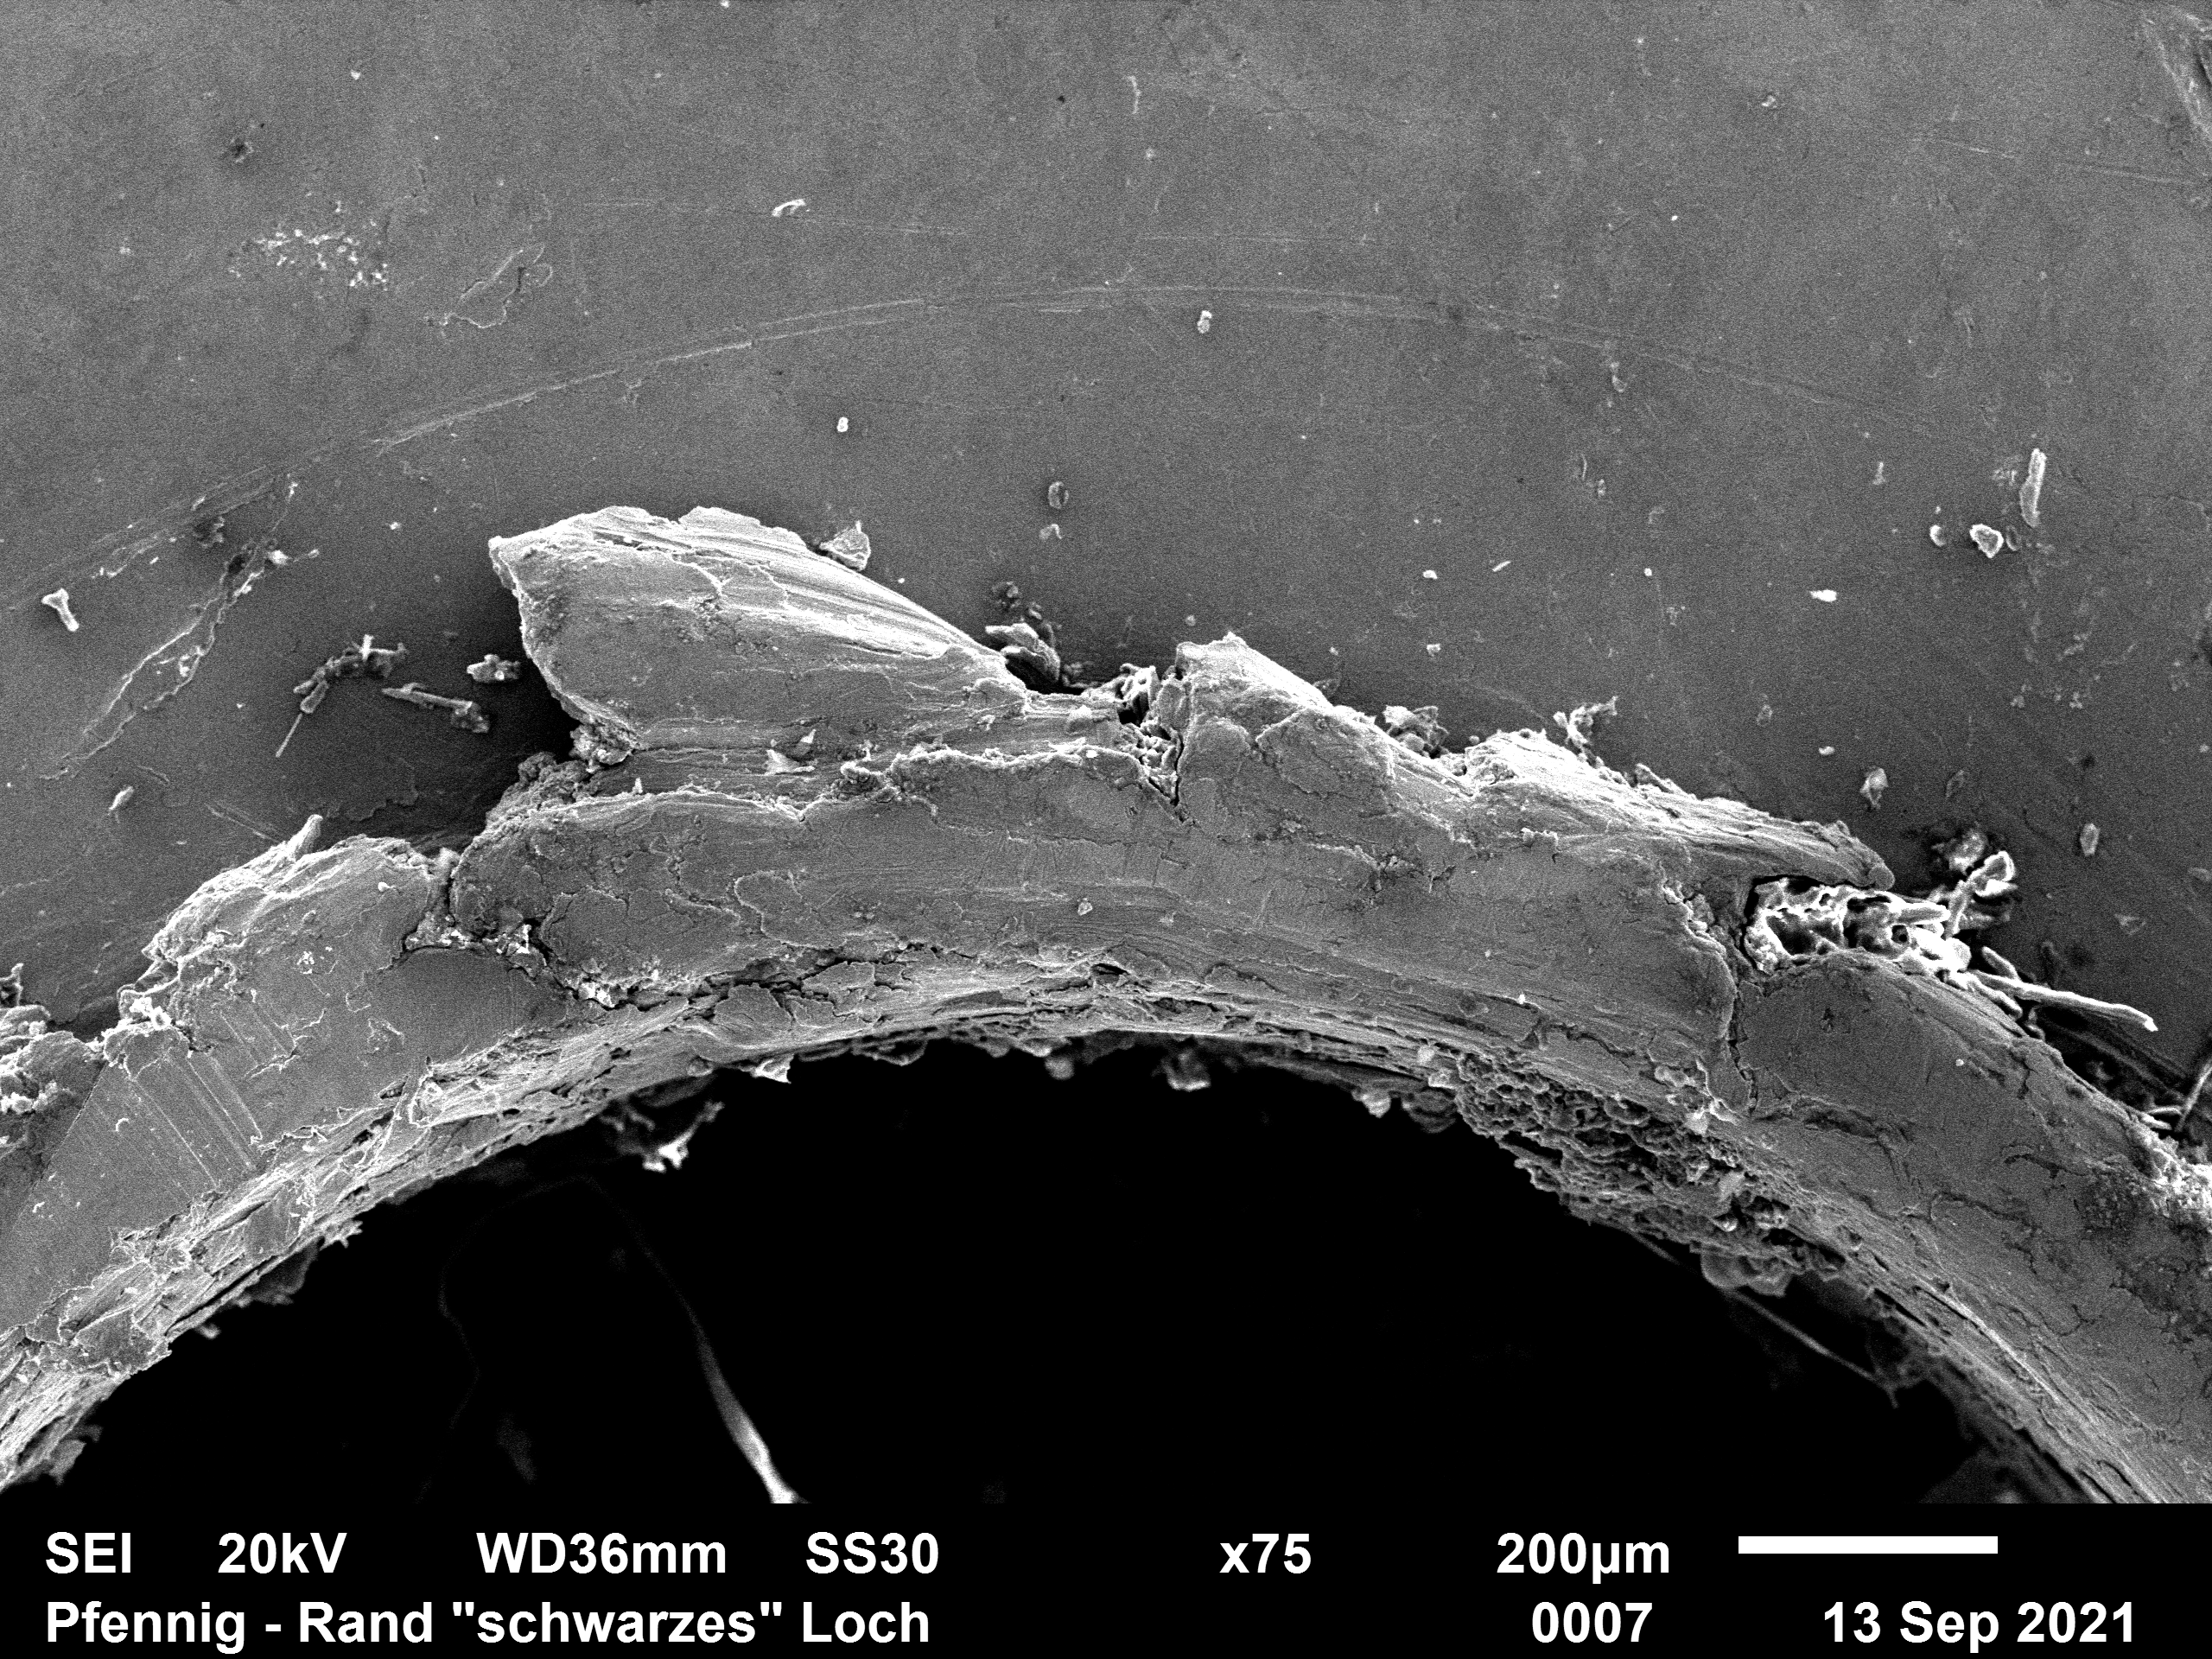
\includegraphics[width=\textwidth]{Auswertung/A/0007.png}
        \caption{$U_B = 20$ kV}
    \end{subfigure}
    \hfill
    \begin{subfigure}[b]{0.45\textwidth}
        \centering
        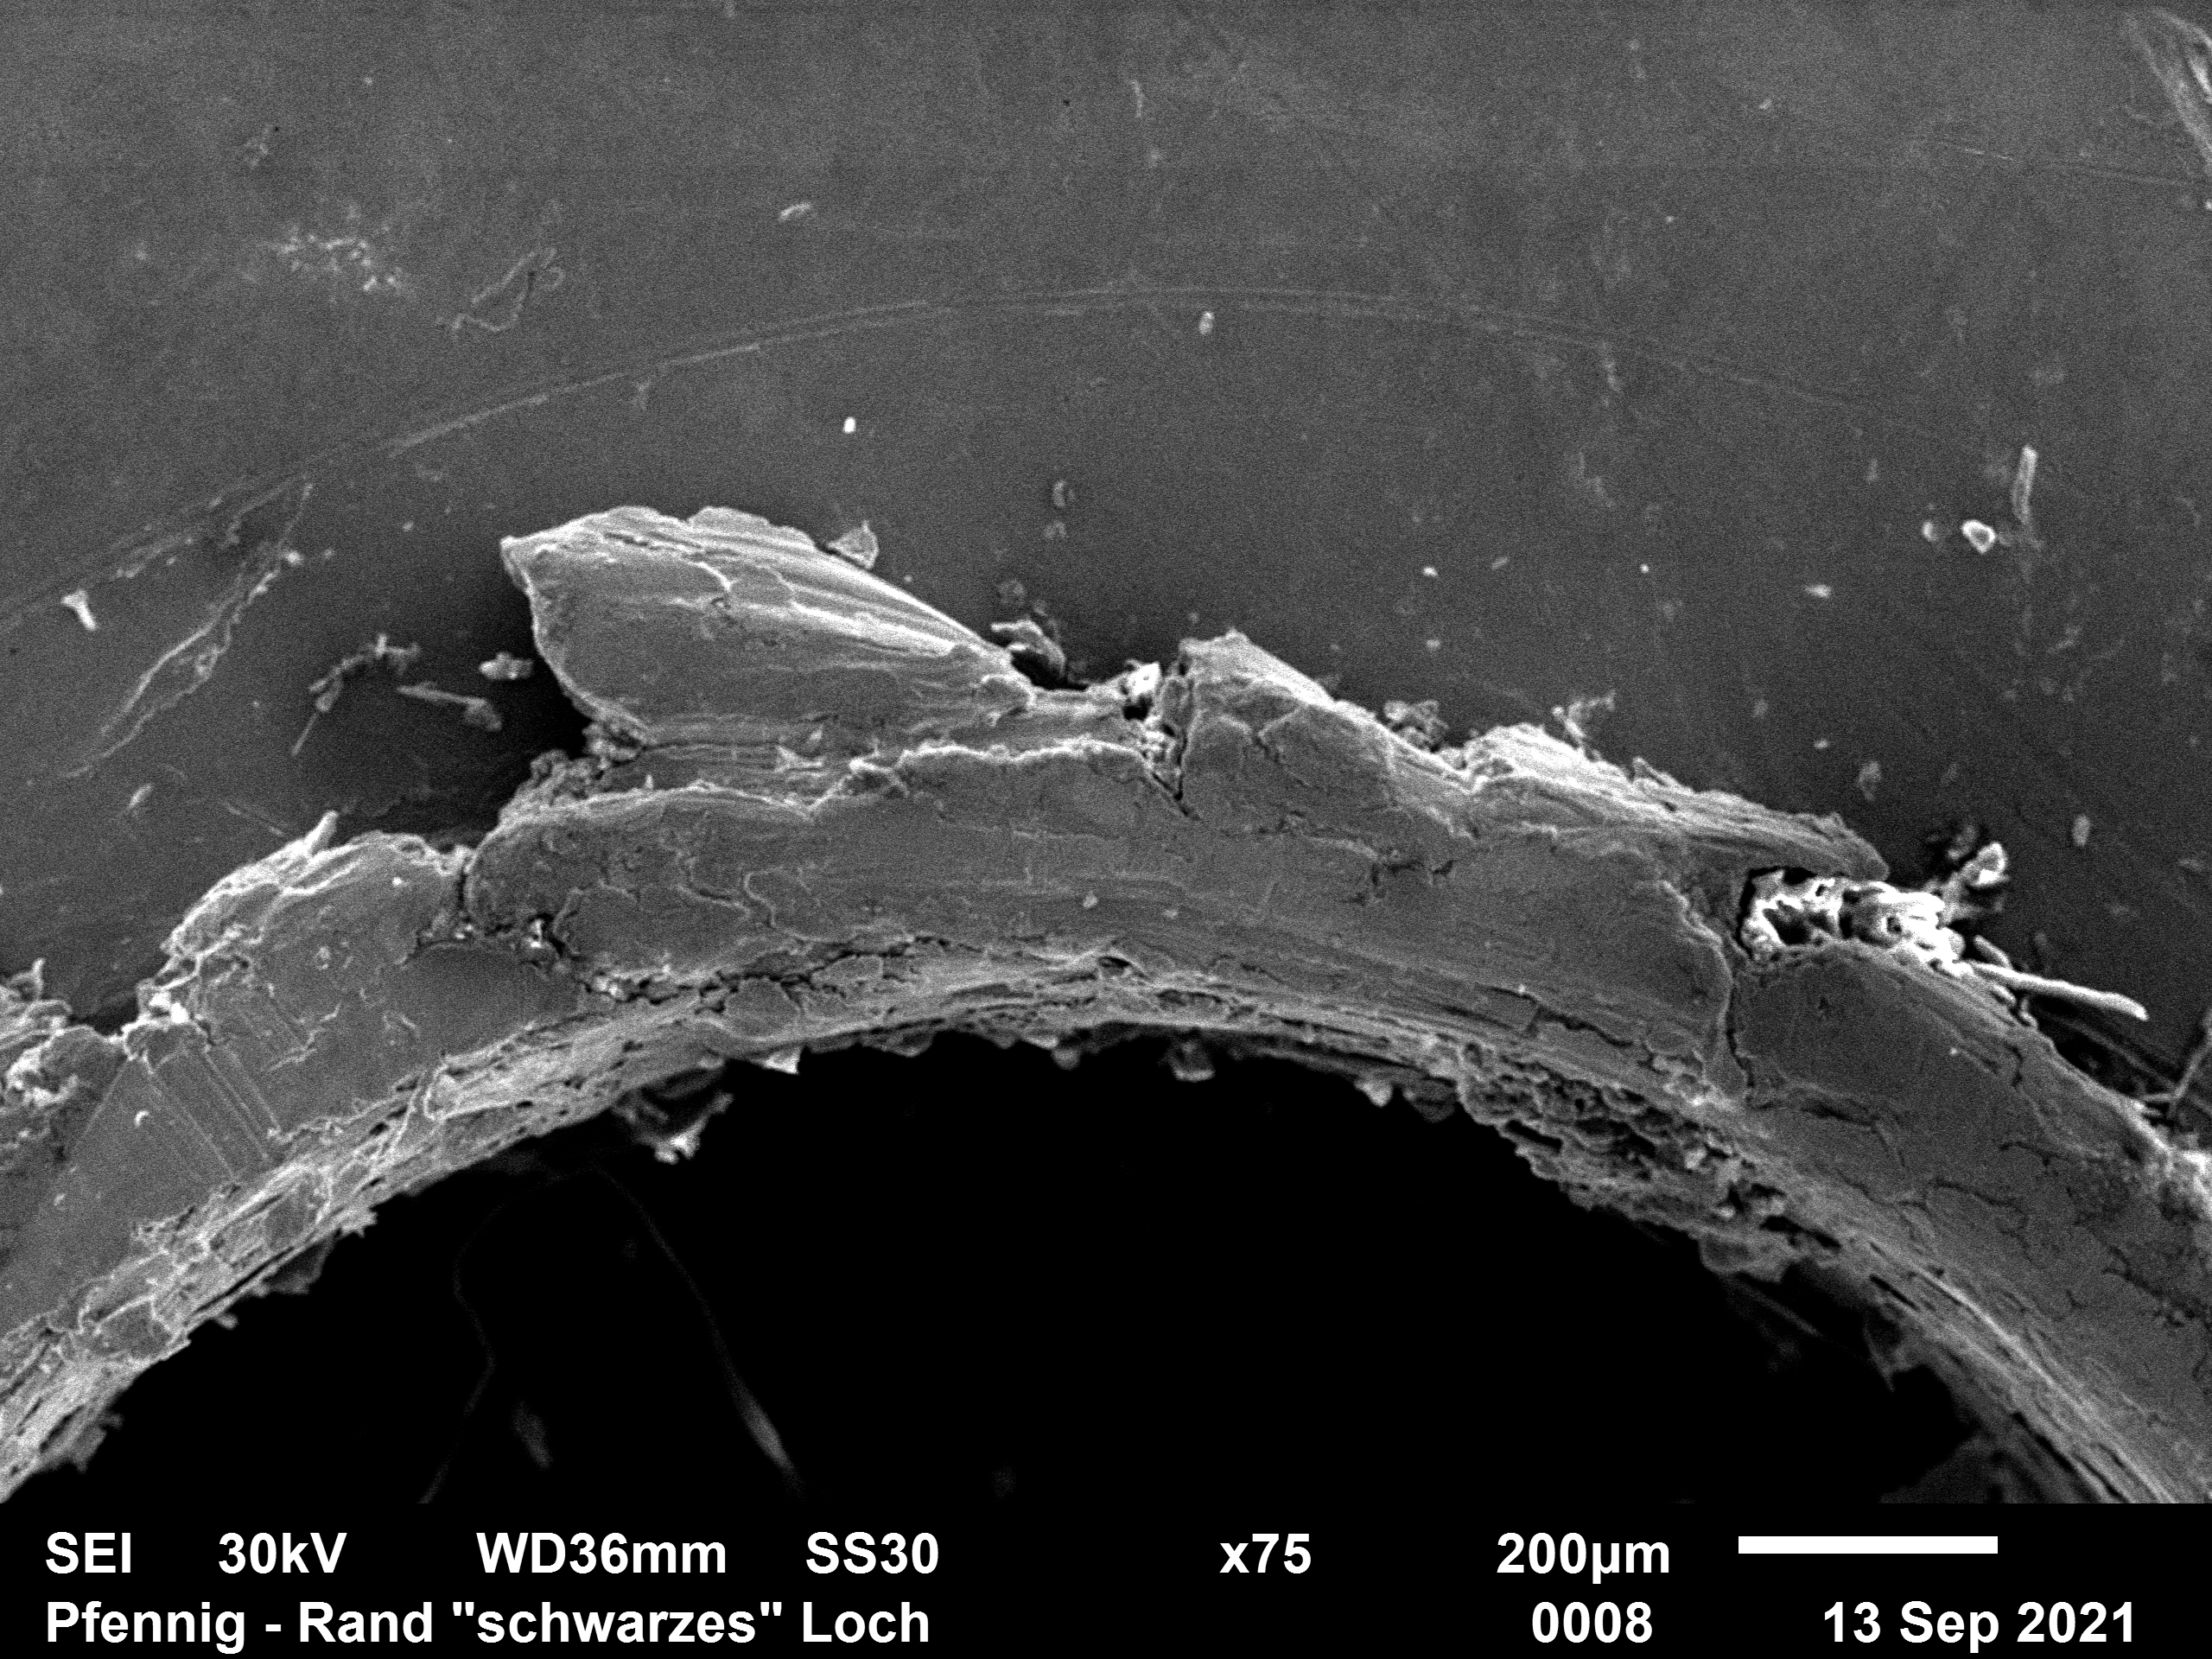
\includegraphics[width=\textwidth]{Auswertung/A/0008.png}
        \caption{$U_B = 30$ kV}
    \end{subfigure}
    \caption{SEI bei unterschiedlichen Beschleunigunsspannungen}
\end{figure}

Für niedrige Spannungen sind zunehmend Flecken auf der glatten Fläche zu erkennen, was möglicherweise durch Verunreinigungen auf der Probenoberfläche verursacht wird, welch bei niedrigerer Energie der Elektronen mehr ins Gewicht fallen. Elektronen mit niedriger Energie werden durch diese Rückstände weiter entschleunigt, weshalb dann dunkle Flecken zu erkennen sind. Die Probe ist im Allgemeinen für höhere Spannungen besser zu erkennen.

\newpage
Als Nächstes wurde der Everhart-Thronley-Detektor im RE Modus (REF) verwendet und dabei ebenfalls die Beschleunigungsspannung variiert.
\begin{figure}[h]
    \centering
    
    \begin{subfigure}[b]{0.45\textwidth}
        \centering
        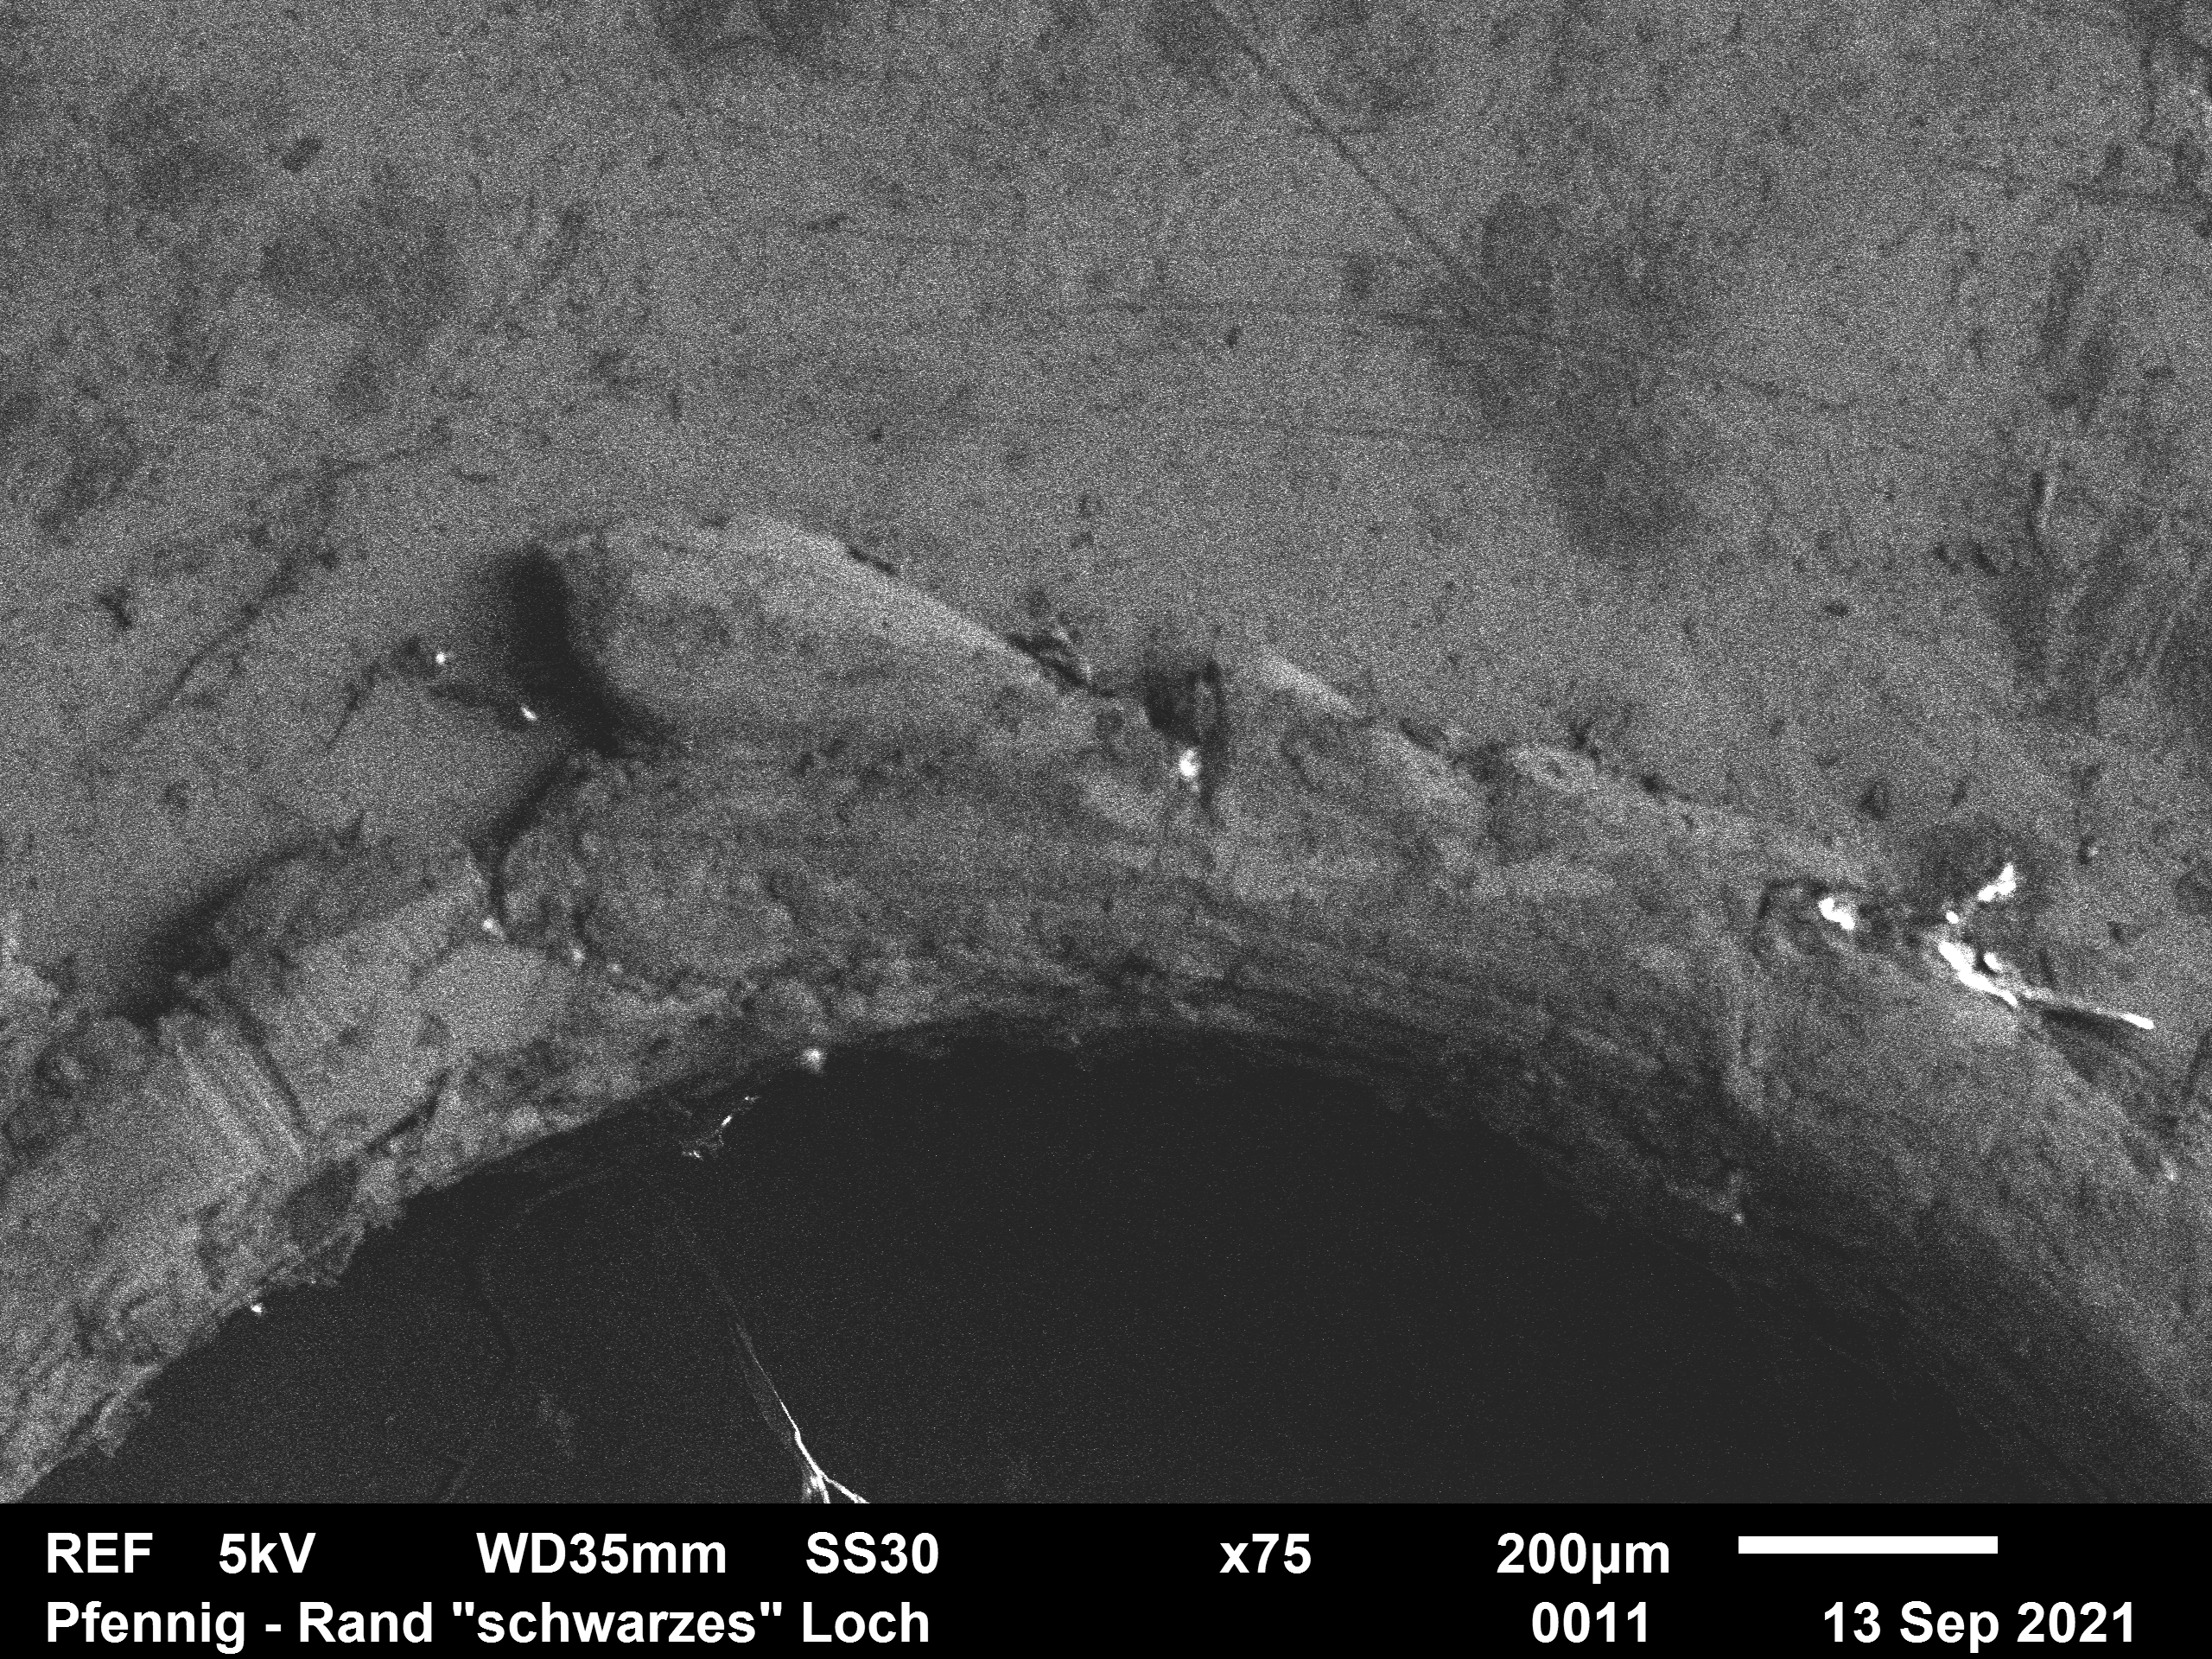
\includegraphics[width=\textwidth]{Auswertung/A/0011.png}
        \caption{$U_B = 5$ kV}
    \end{subfigure}
    \hfill
    \begin{subfigure}[b]{0.45\textwidth}
        \centering
        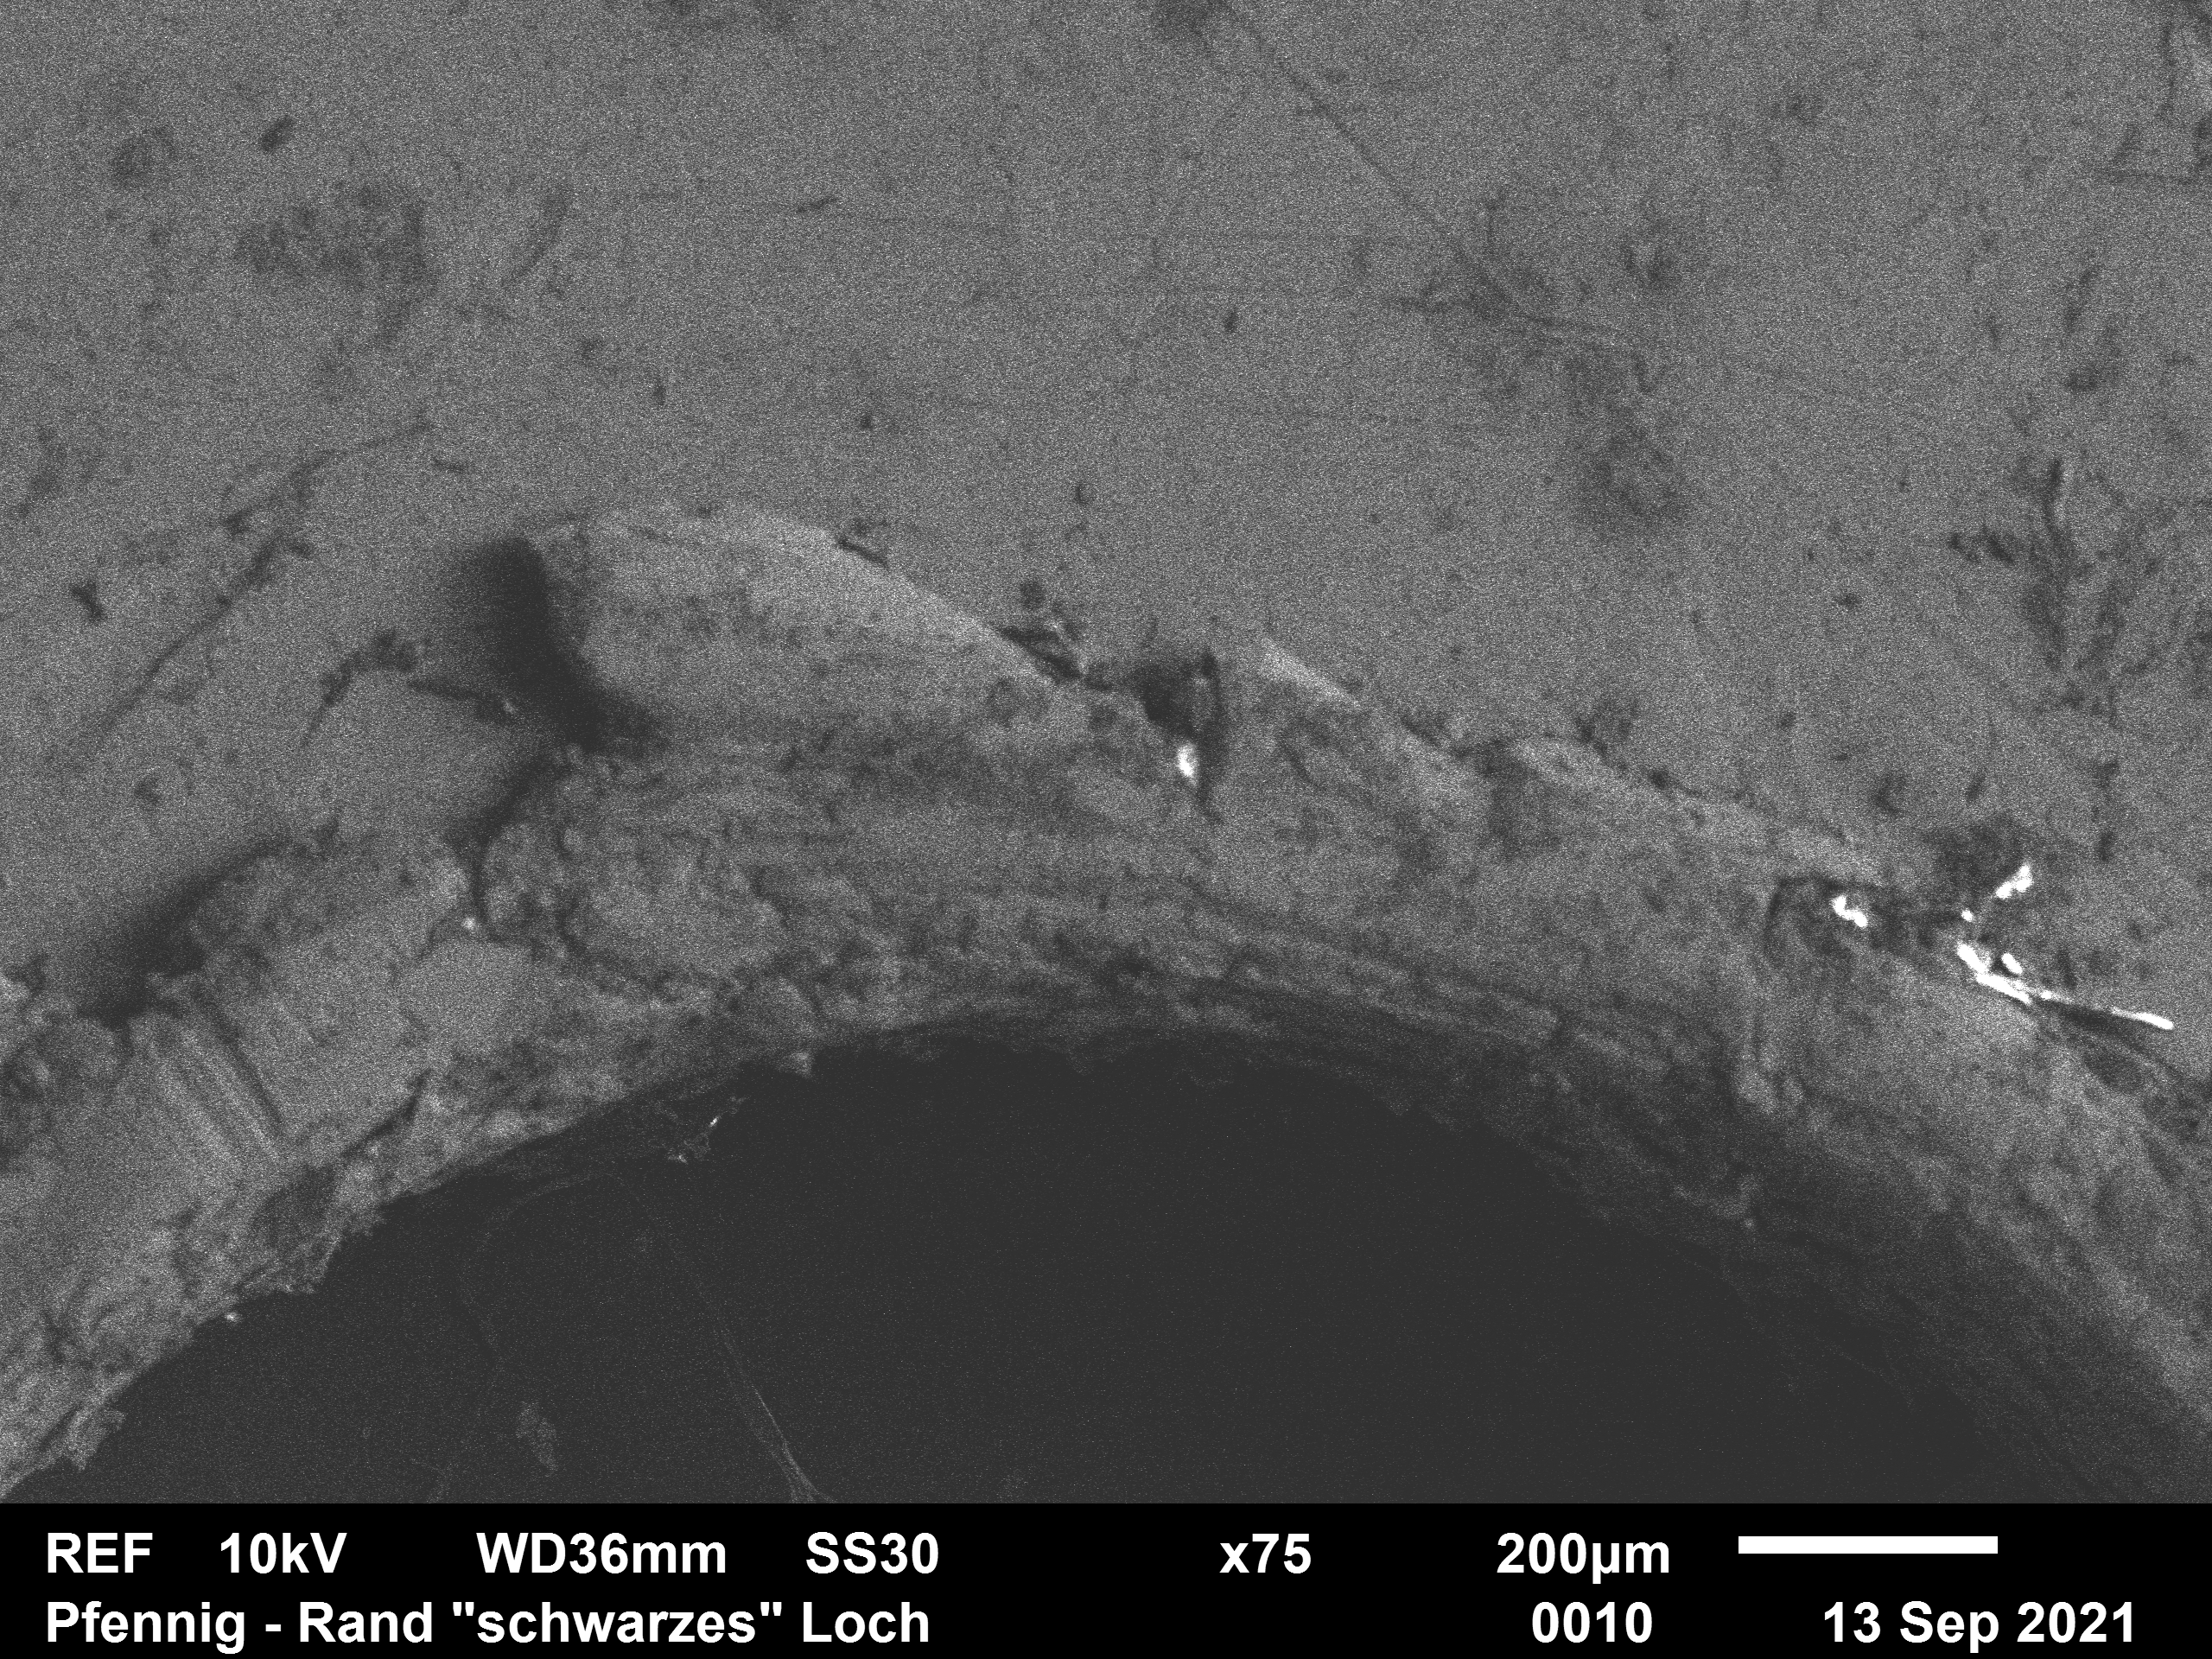
\includegraphics[width=\textwidth]{Auswertung/A/0010.png}
        \caption{$U_B = 10$ kV}
    \end{subfigure}
    \\
    \begin{subfigure}[b]{0.45\textwidth}
        \centering
        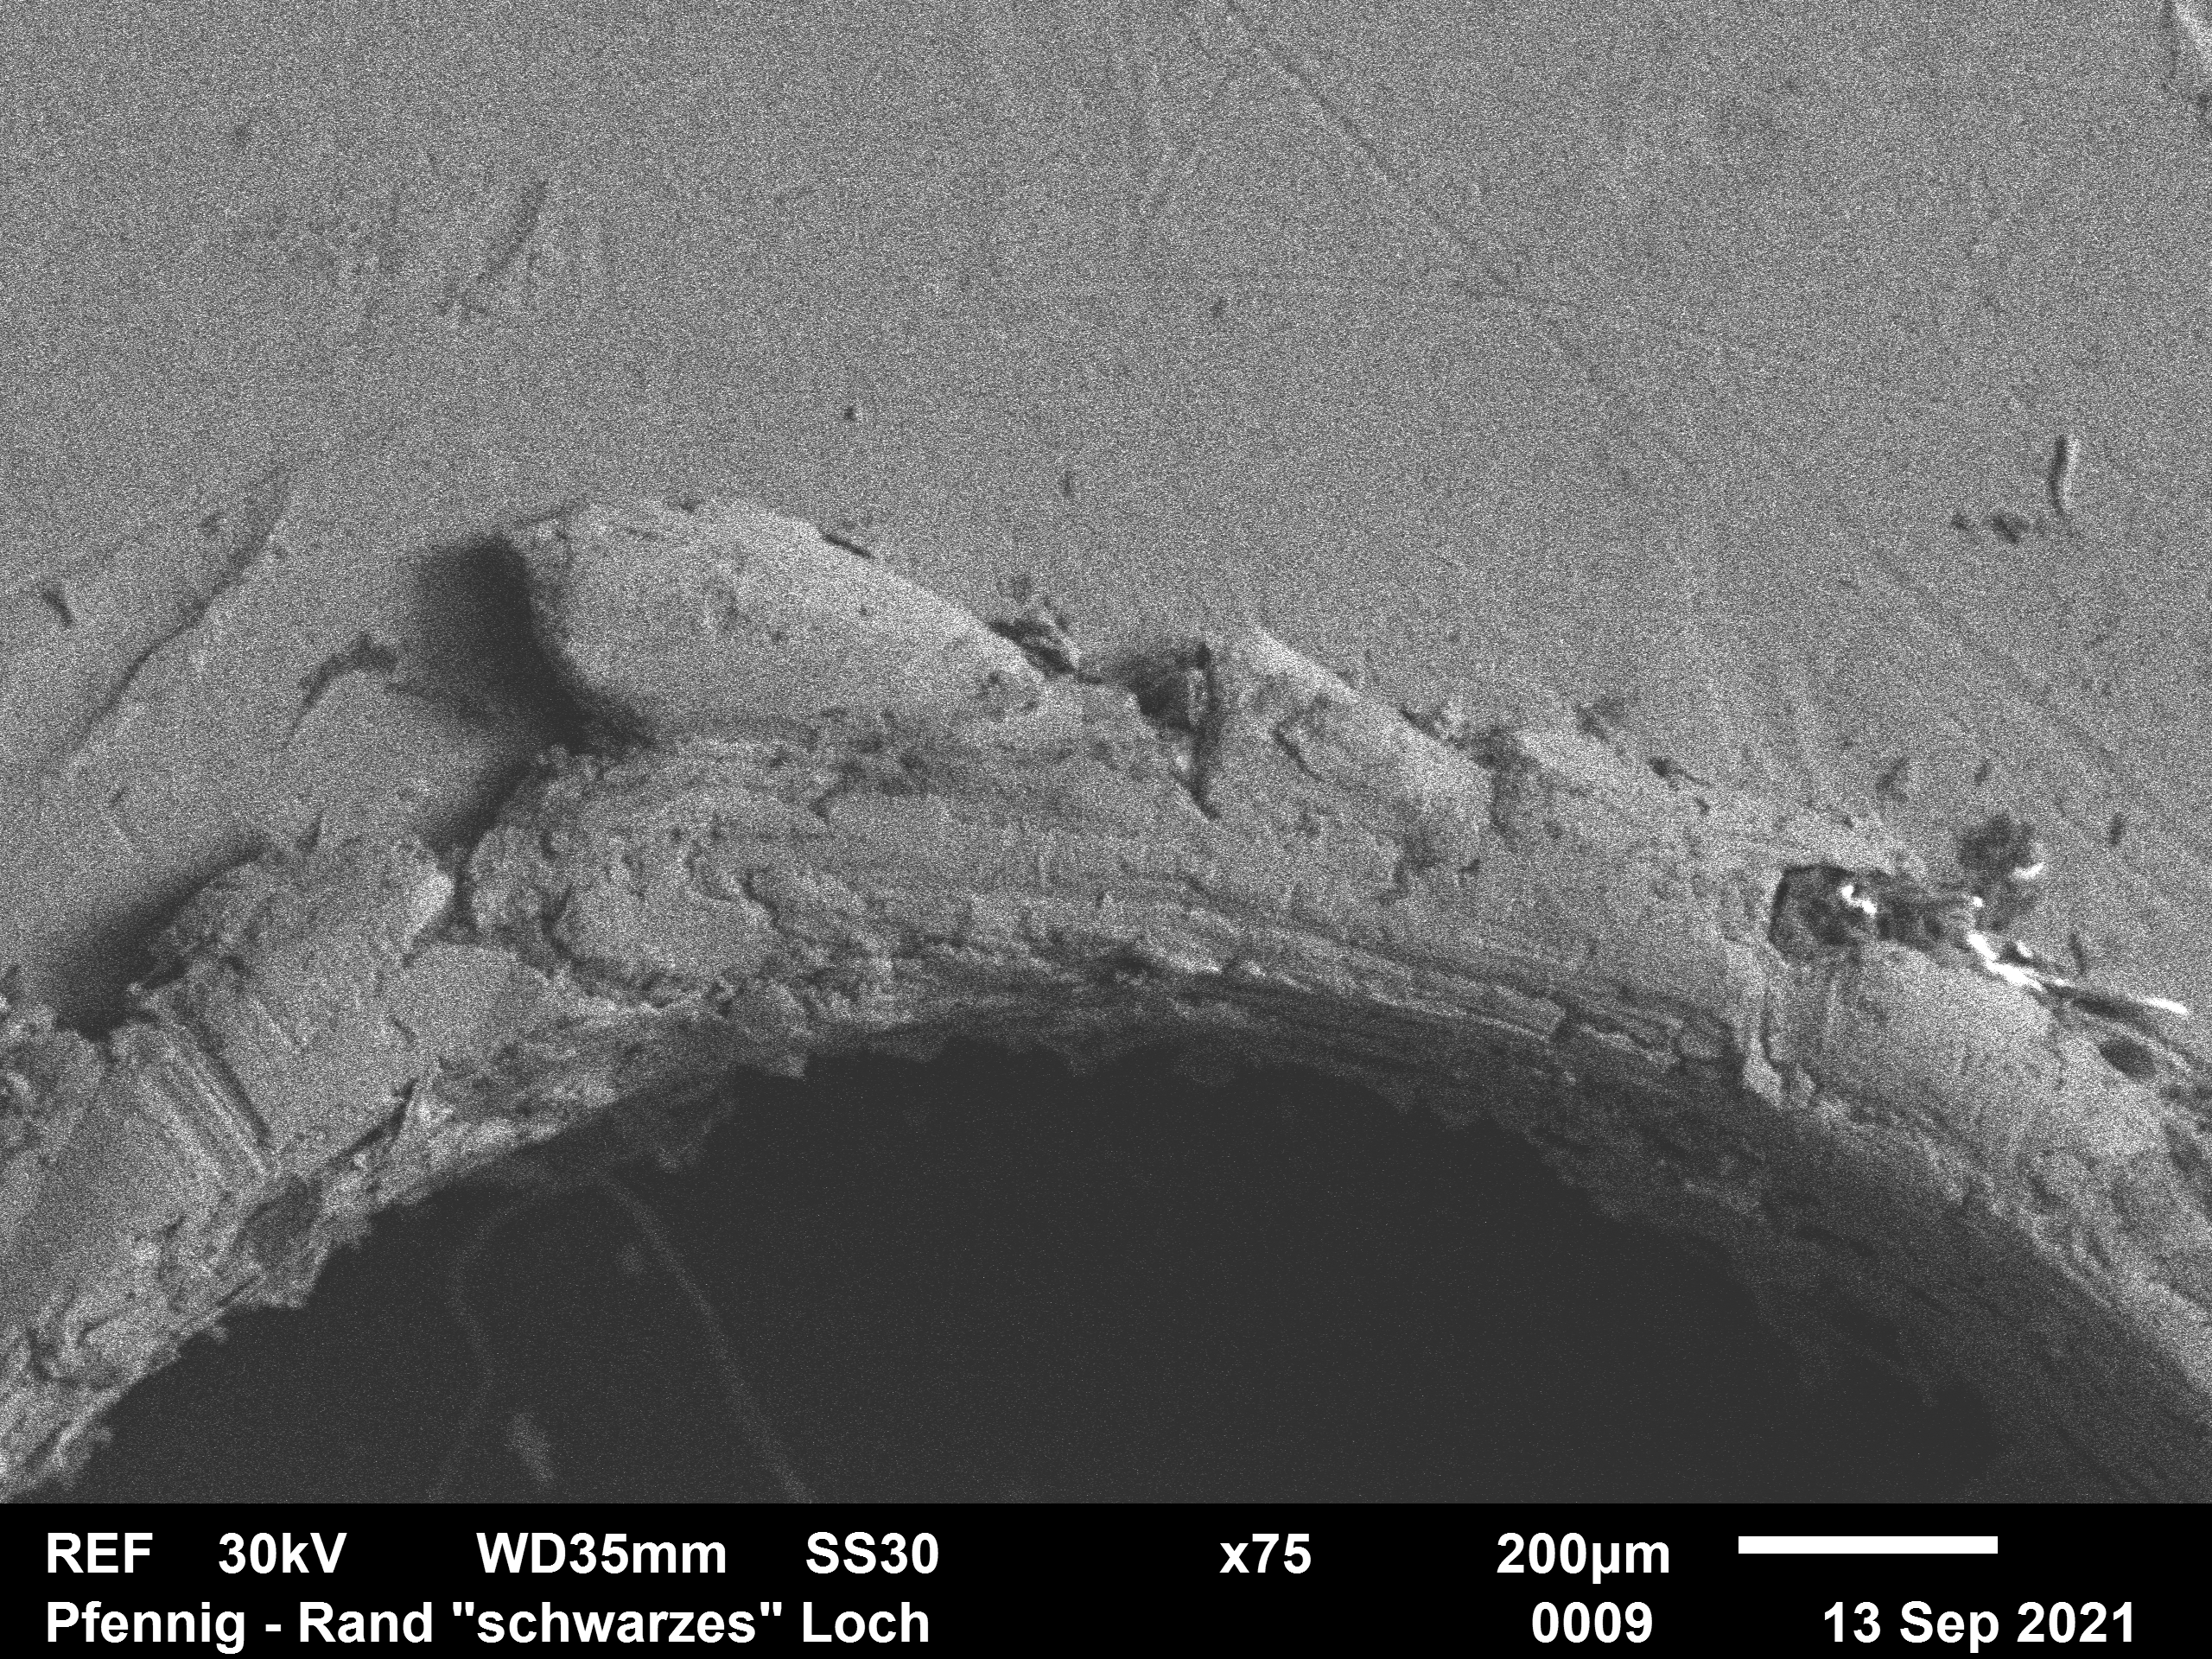
\includegraphics[width=\textwidth]{Auswertung/A/0009.png}
        \caption{$U_B = 30$ kV}
    \end{subfigure}
    \caption{REF bei unterschiedlichen Beschleunigunsspannungen}
\end{figure}

Genau wie oben, im Abschnitt \ref{subsec:Bs}, sind auch im REF Betrieb bei niedriger Energie der Primärelektronen dunkle Flecken zu erkennen. Auch ist das Bild für kleinere Beschleunigungsspannungen verschwommener.\\
Weiterhin sind Abschattungskontraste im Bild zu erkennen, was mit dem verwendeten Betriebsmodus zusammenhängt. Das Zustandekommen dieses Effektes wird in Abschnitt \ref{sec:kontrast} genauer erklärt. \\


\newpage
Das gleich wurde auch für den Halbleiterdetektor im Compo-Mode (BEC) gemacht.
\begin{figure}[h]
    \centering
    
    \begin{subfigure}[b]{0.45\textwidth}
        \centering
        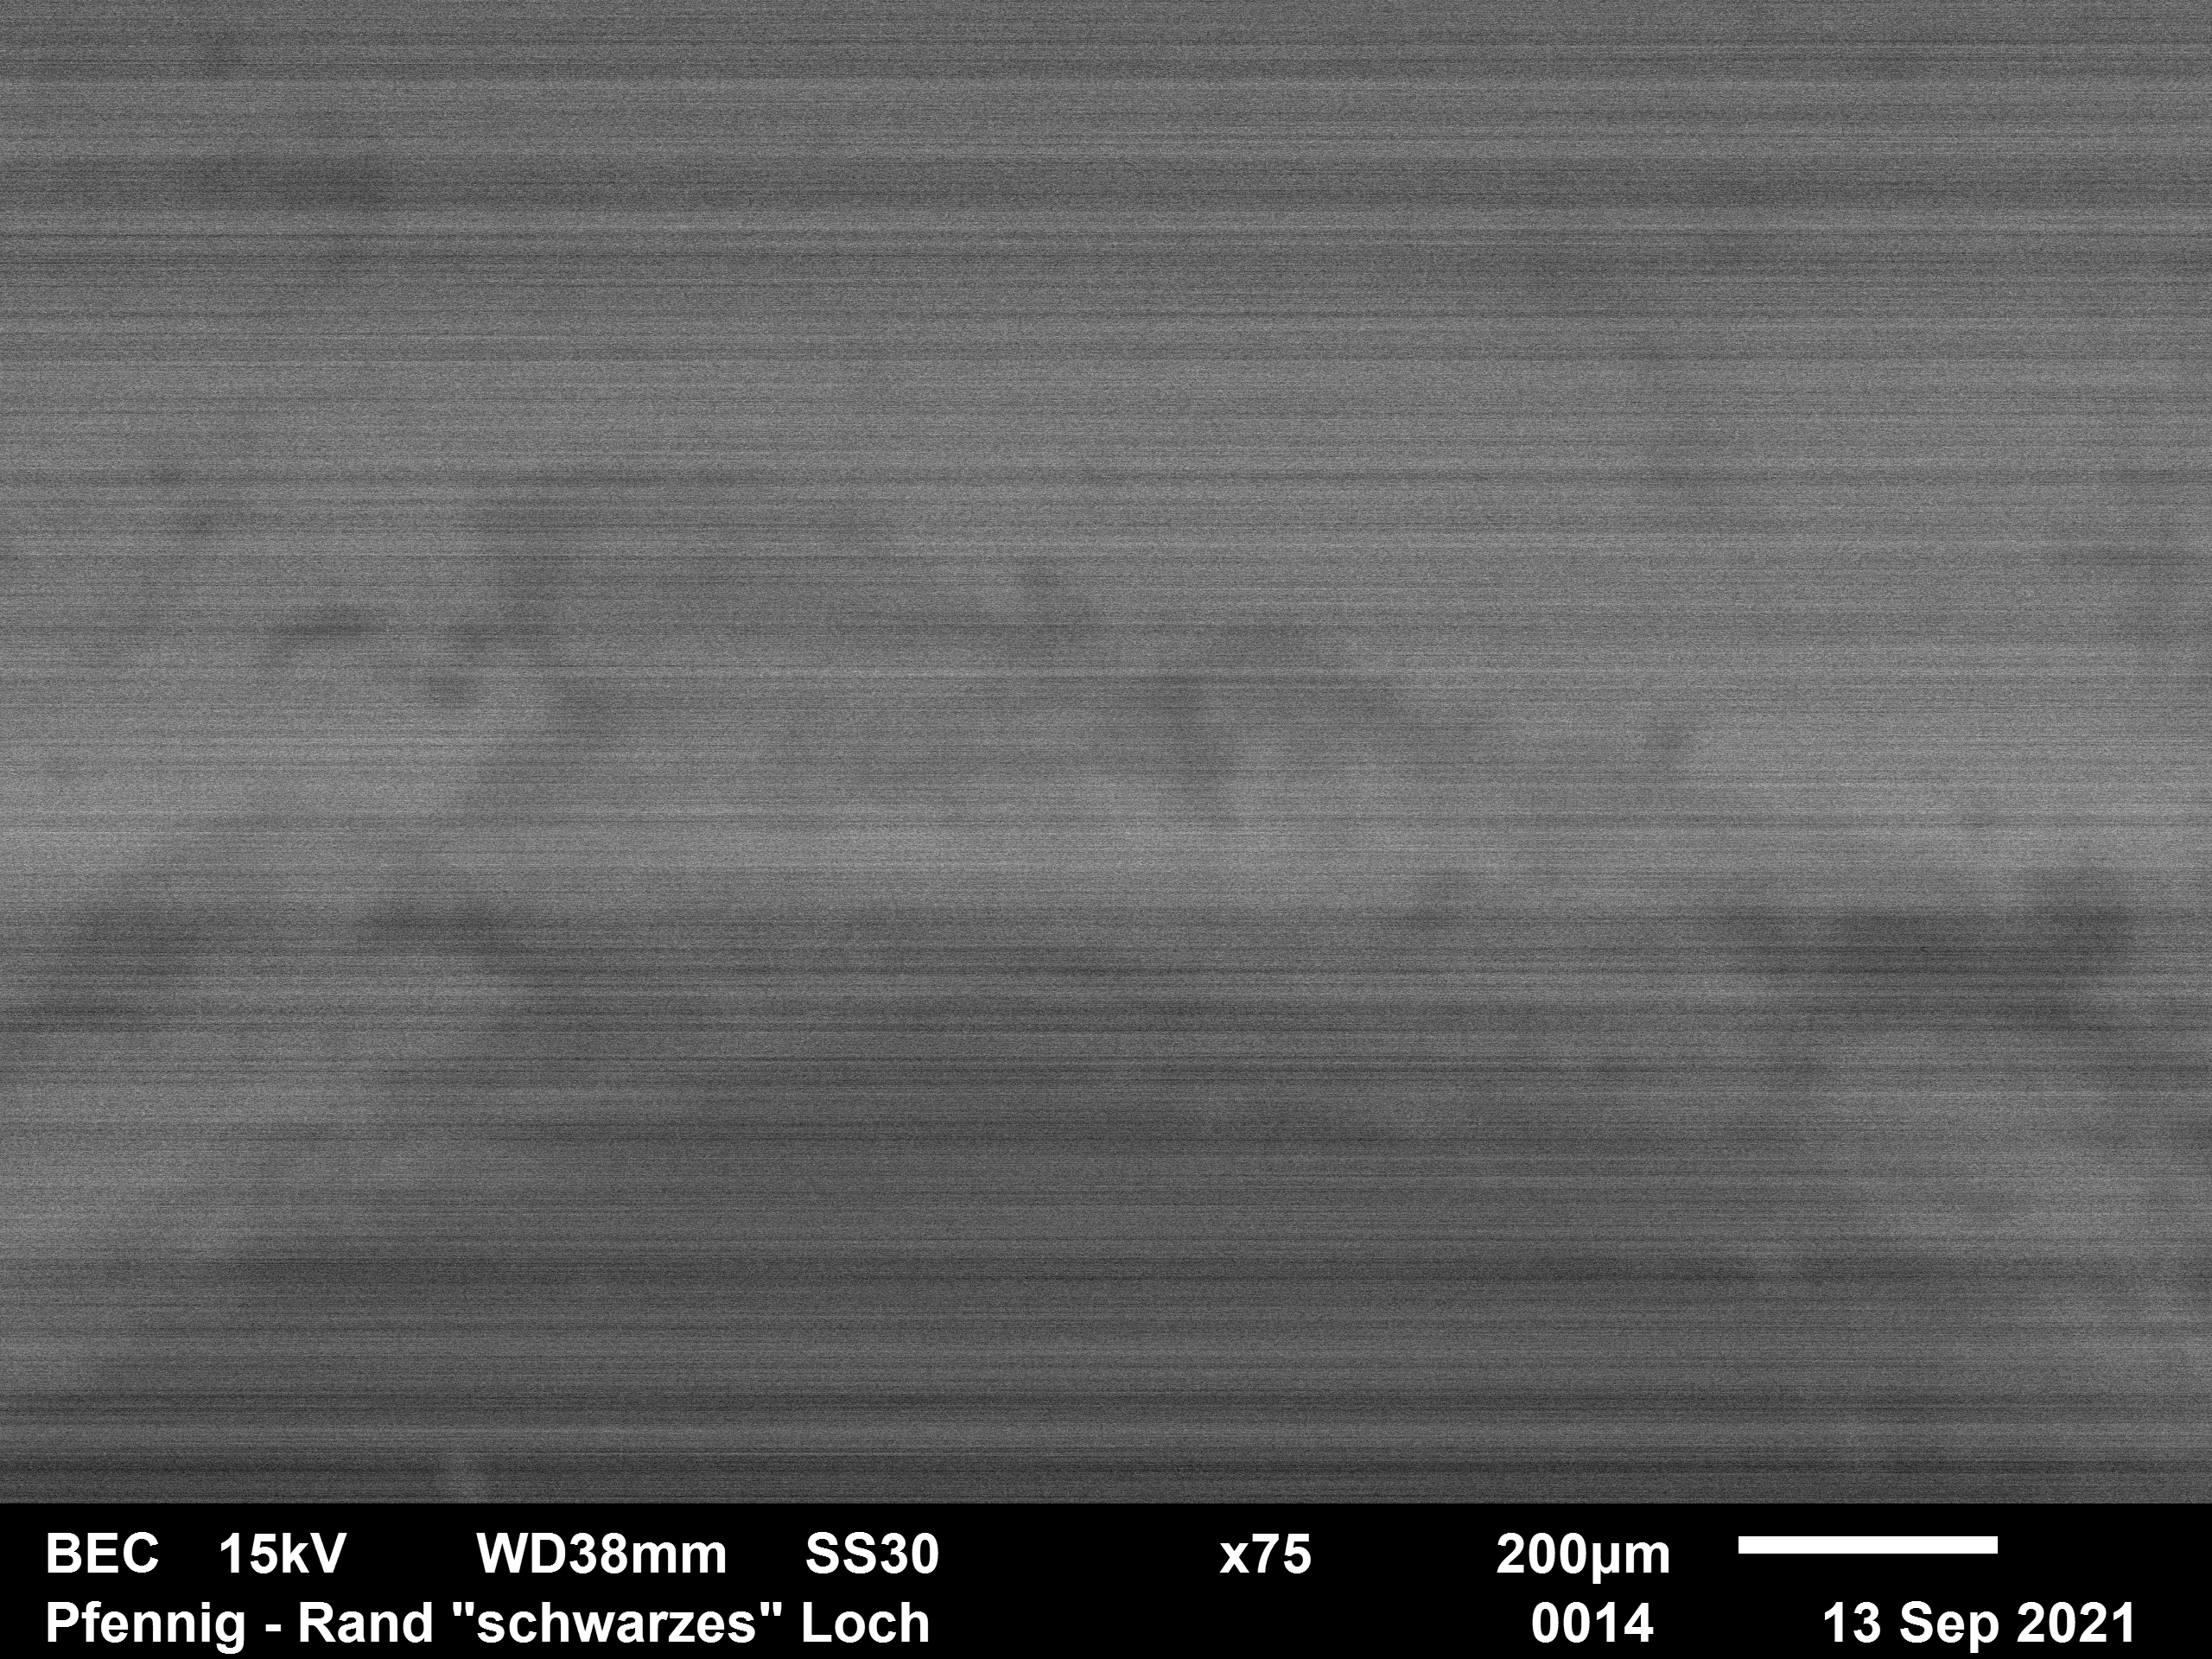
\includegraphics[width=\textwidth]{Auswertung/A/0014.png}
        \caption{$U_B = 15$ kV}
    \end{subfigure}
    \hfill
    \begin{subfigure}[b]{0.45\textwidth}
        \centering
        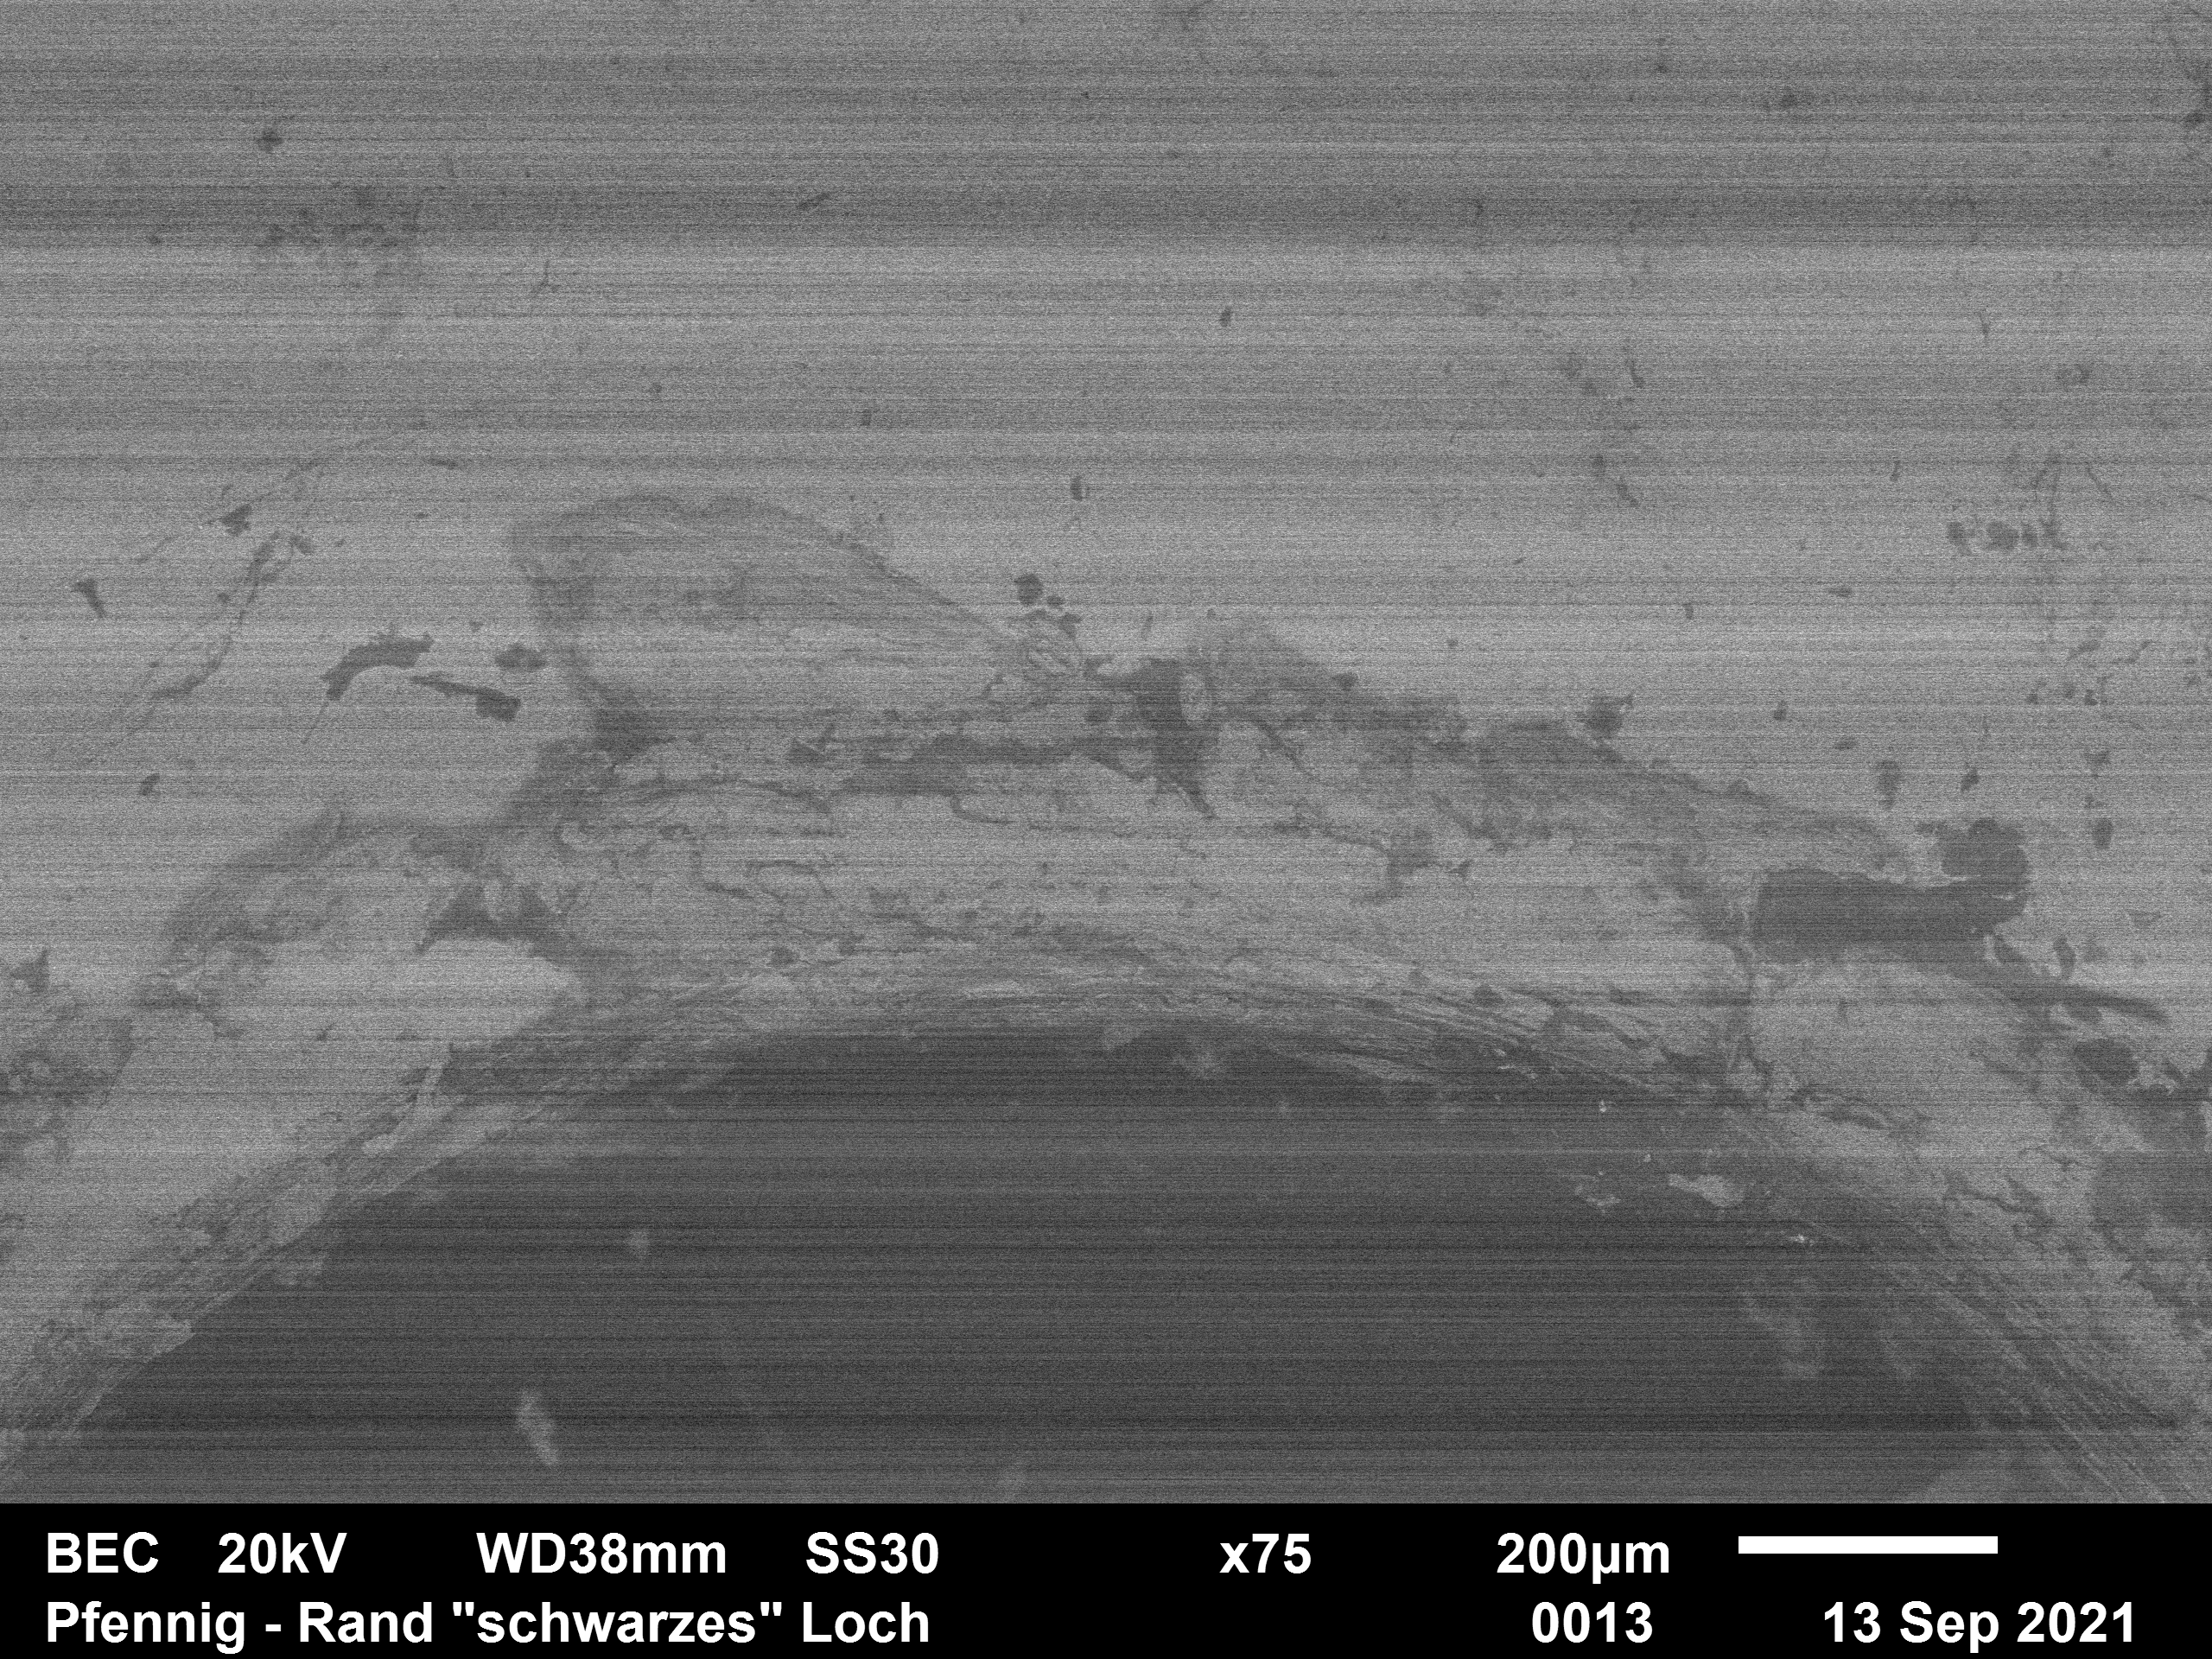
\includegraphics[width=\textwidth]{Auswertung/A/0013.png}
        \caption{$U_B = 20$ kV}
    \end{subfigure}
    \\
    \begin{subfigure}[b]{0.45\textwidth}
        \centering
        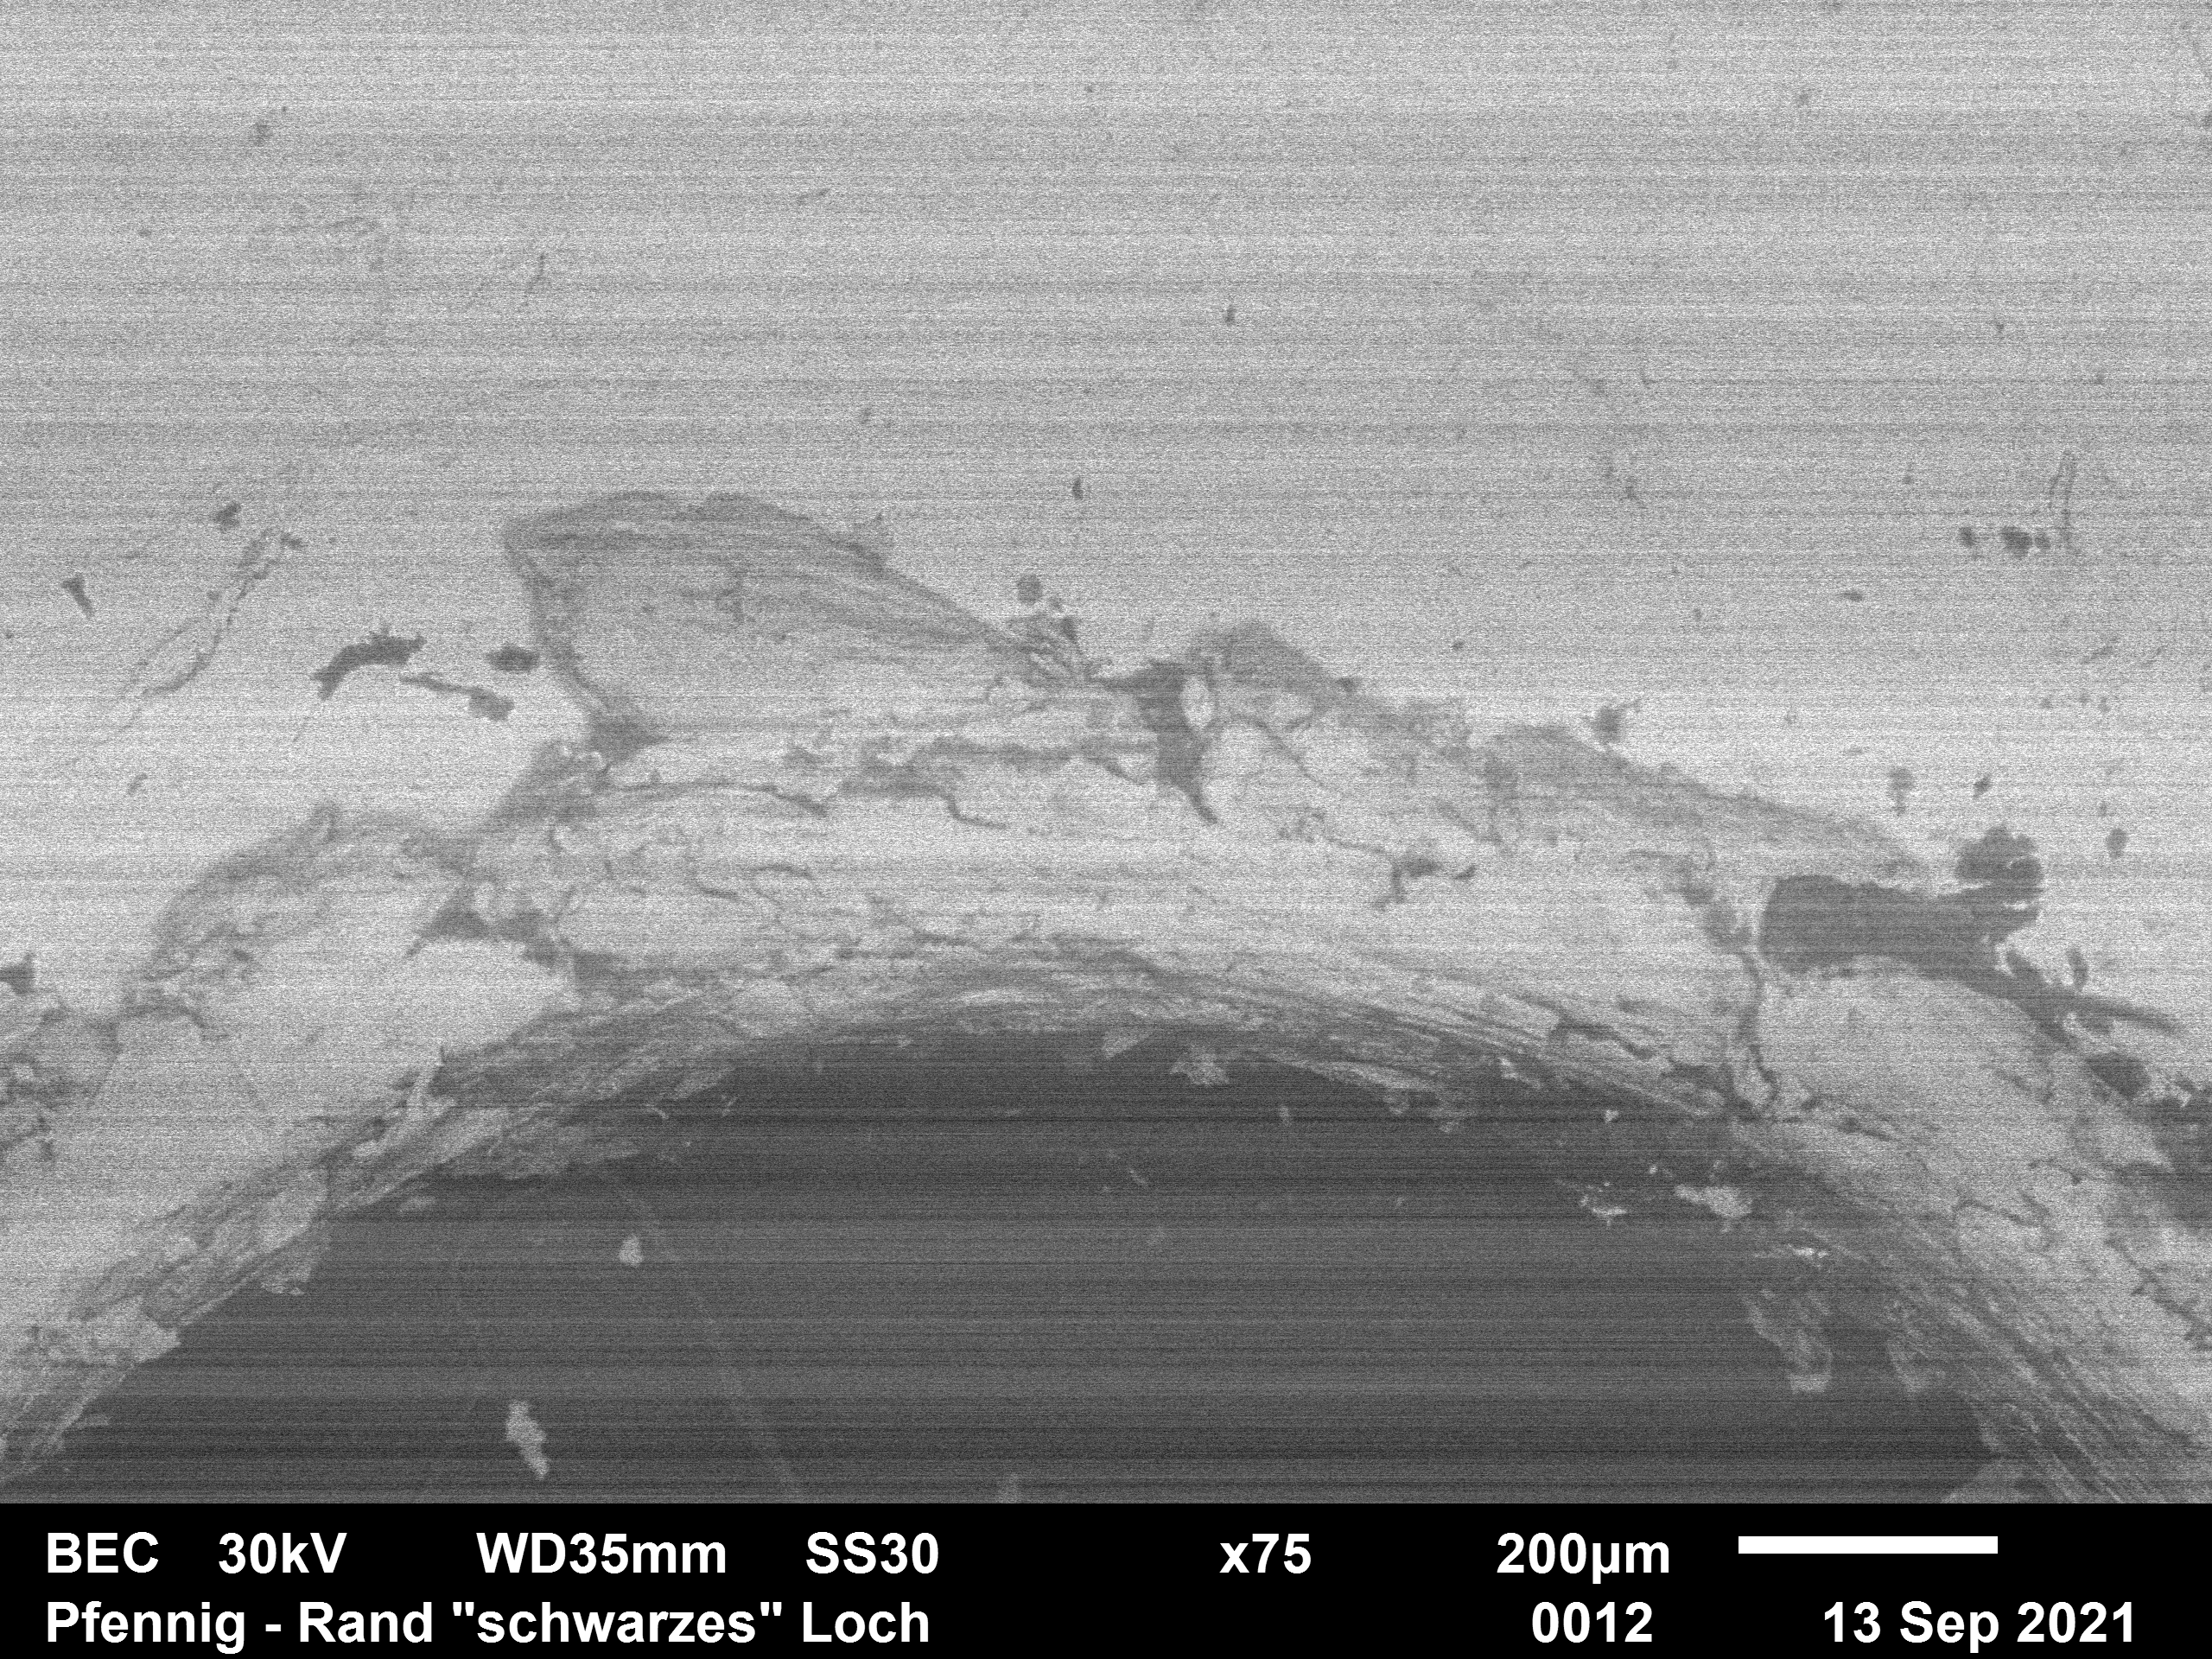
\includegraphics[width=\textwidth]{Auswertung/A/0012.png}
        \caption{$U_B = 30$ kV}
    \end{subfigure}
    \caption{BEC bei unterschiedlichen Beschleunigunsspannungen}
\end{figure}

Hier fällt sofort auf, dass die Bildqualität rapide mit der Beschleunigungsspannung abfällt. Also muss ein PE Strahl mit niedriger Energie weniger Rückstreuelektronen erzeugen, welche den Halbleiterdetektor erreichen. Außerdem ist aufgrund des Compomodus, welcher wie in Abschnitt \ref{sec:kontrast} erklärt wird Materialunterschieden deutlich macht, erkennbar, dass sich das Loch deutlich abzeichnet.

\newpage
Auch für den Halbleiterdetektor im Topo-Mode (BET) wurde die Beschleunigungsspannung variiert.
\begin{figure}[h]
    \centering
    
    \begin{subfigure}[b]{0.45\textwidth}
        \centering
        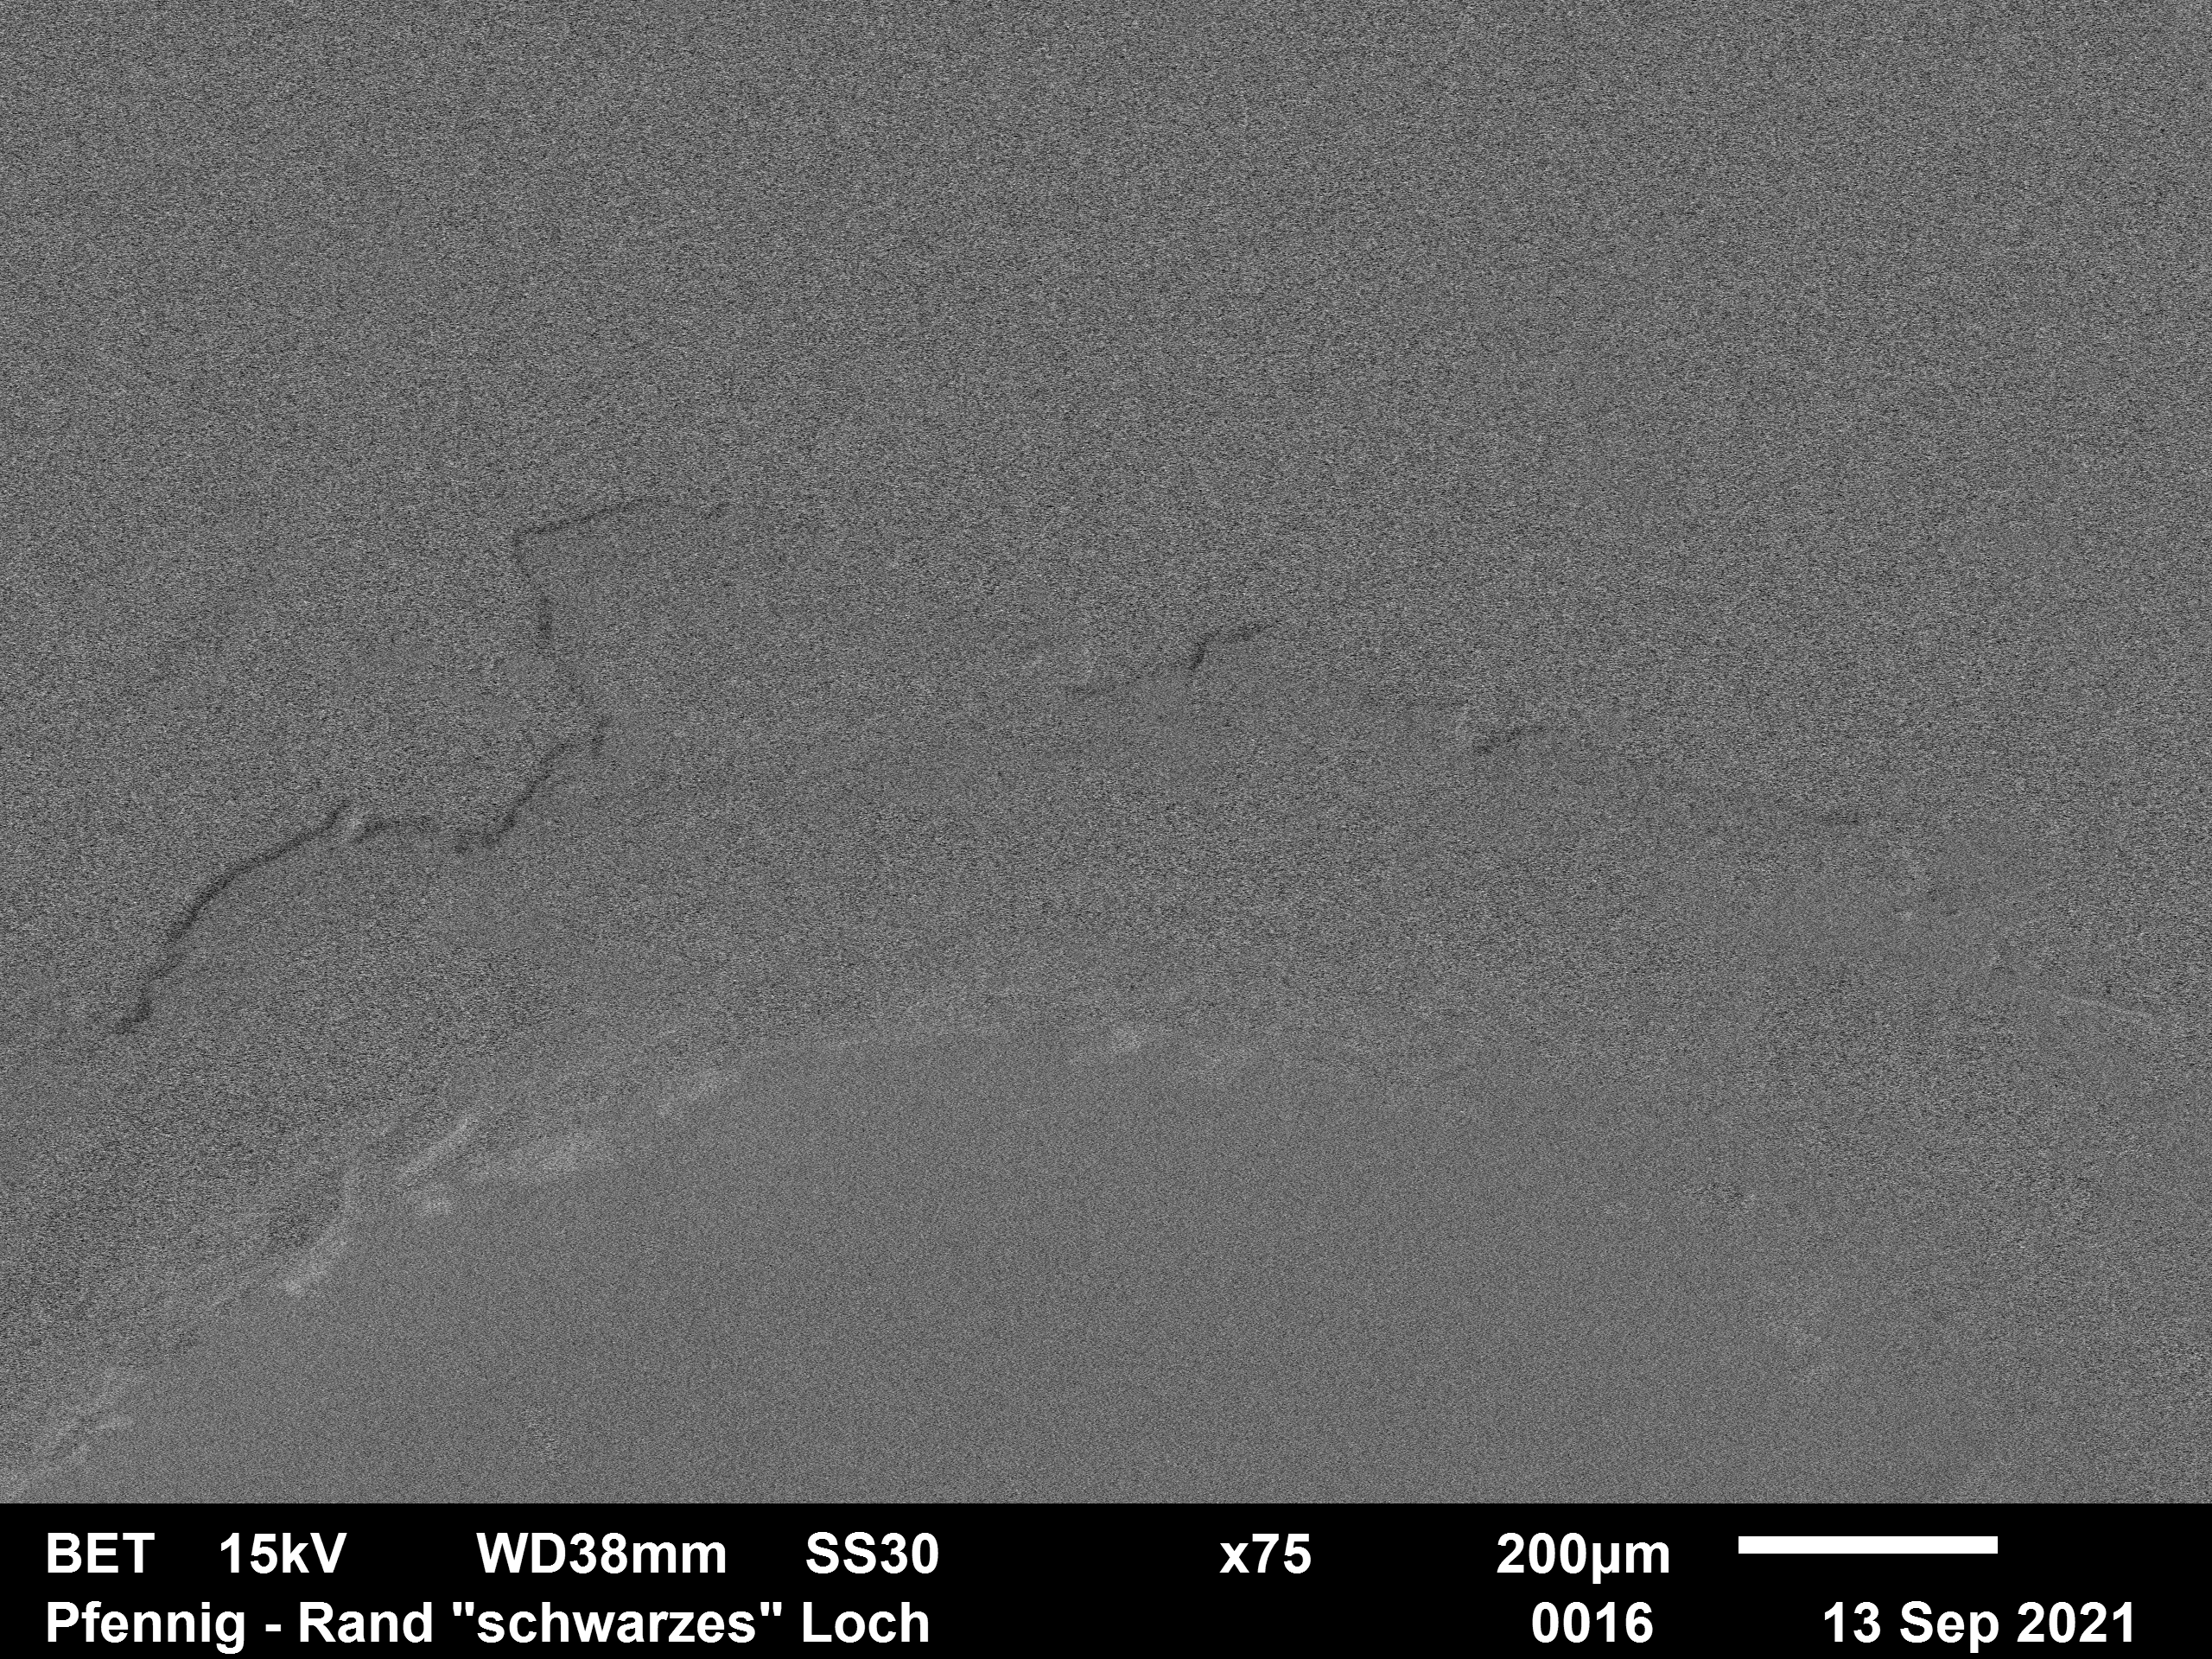
\includegraphics[width=\textwidth]{Auswertung/A/0016.png}
        \caption{$U_B = 15$ kV}
    \end{subfigure}
    \hfill
    \begin{subfigure}[b]{0.45\textwidth}
        \centering
        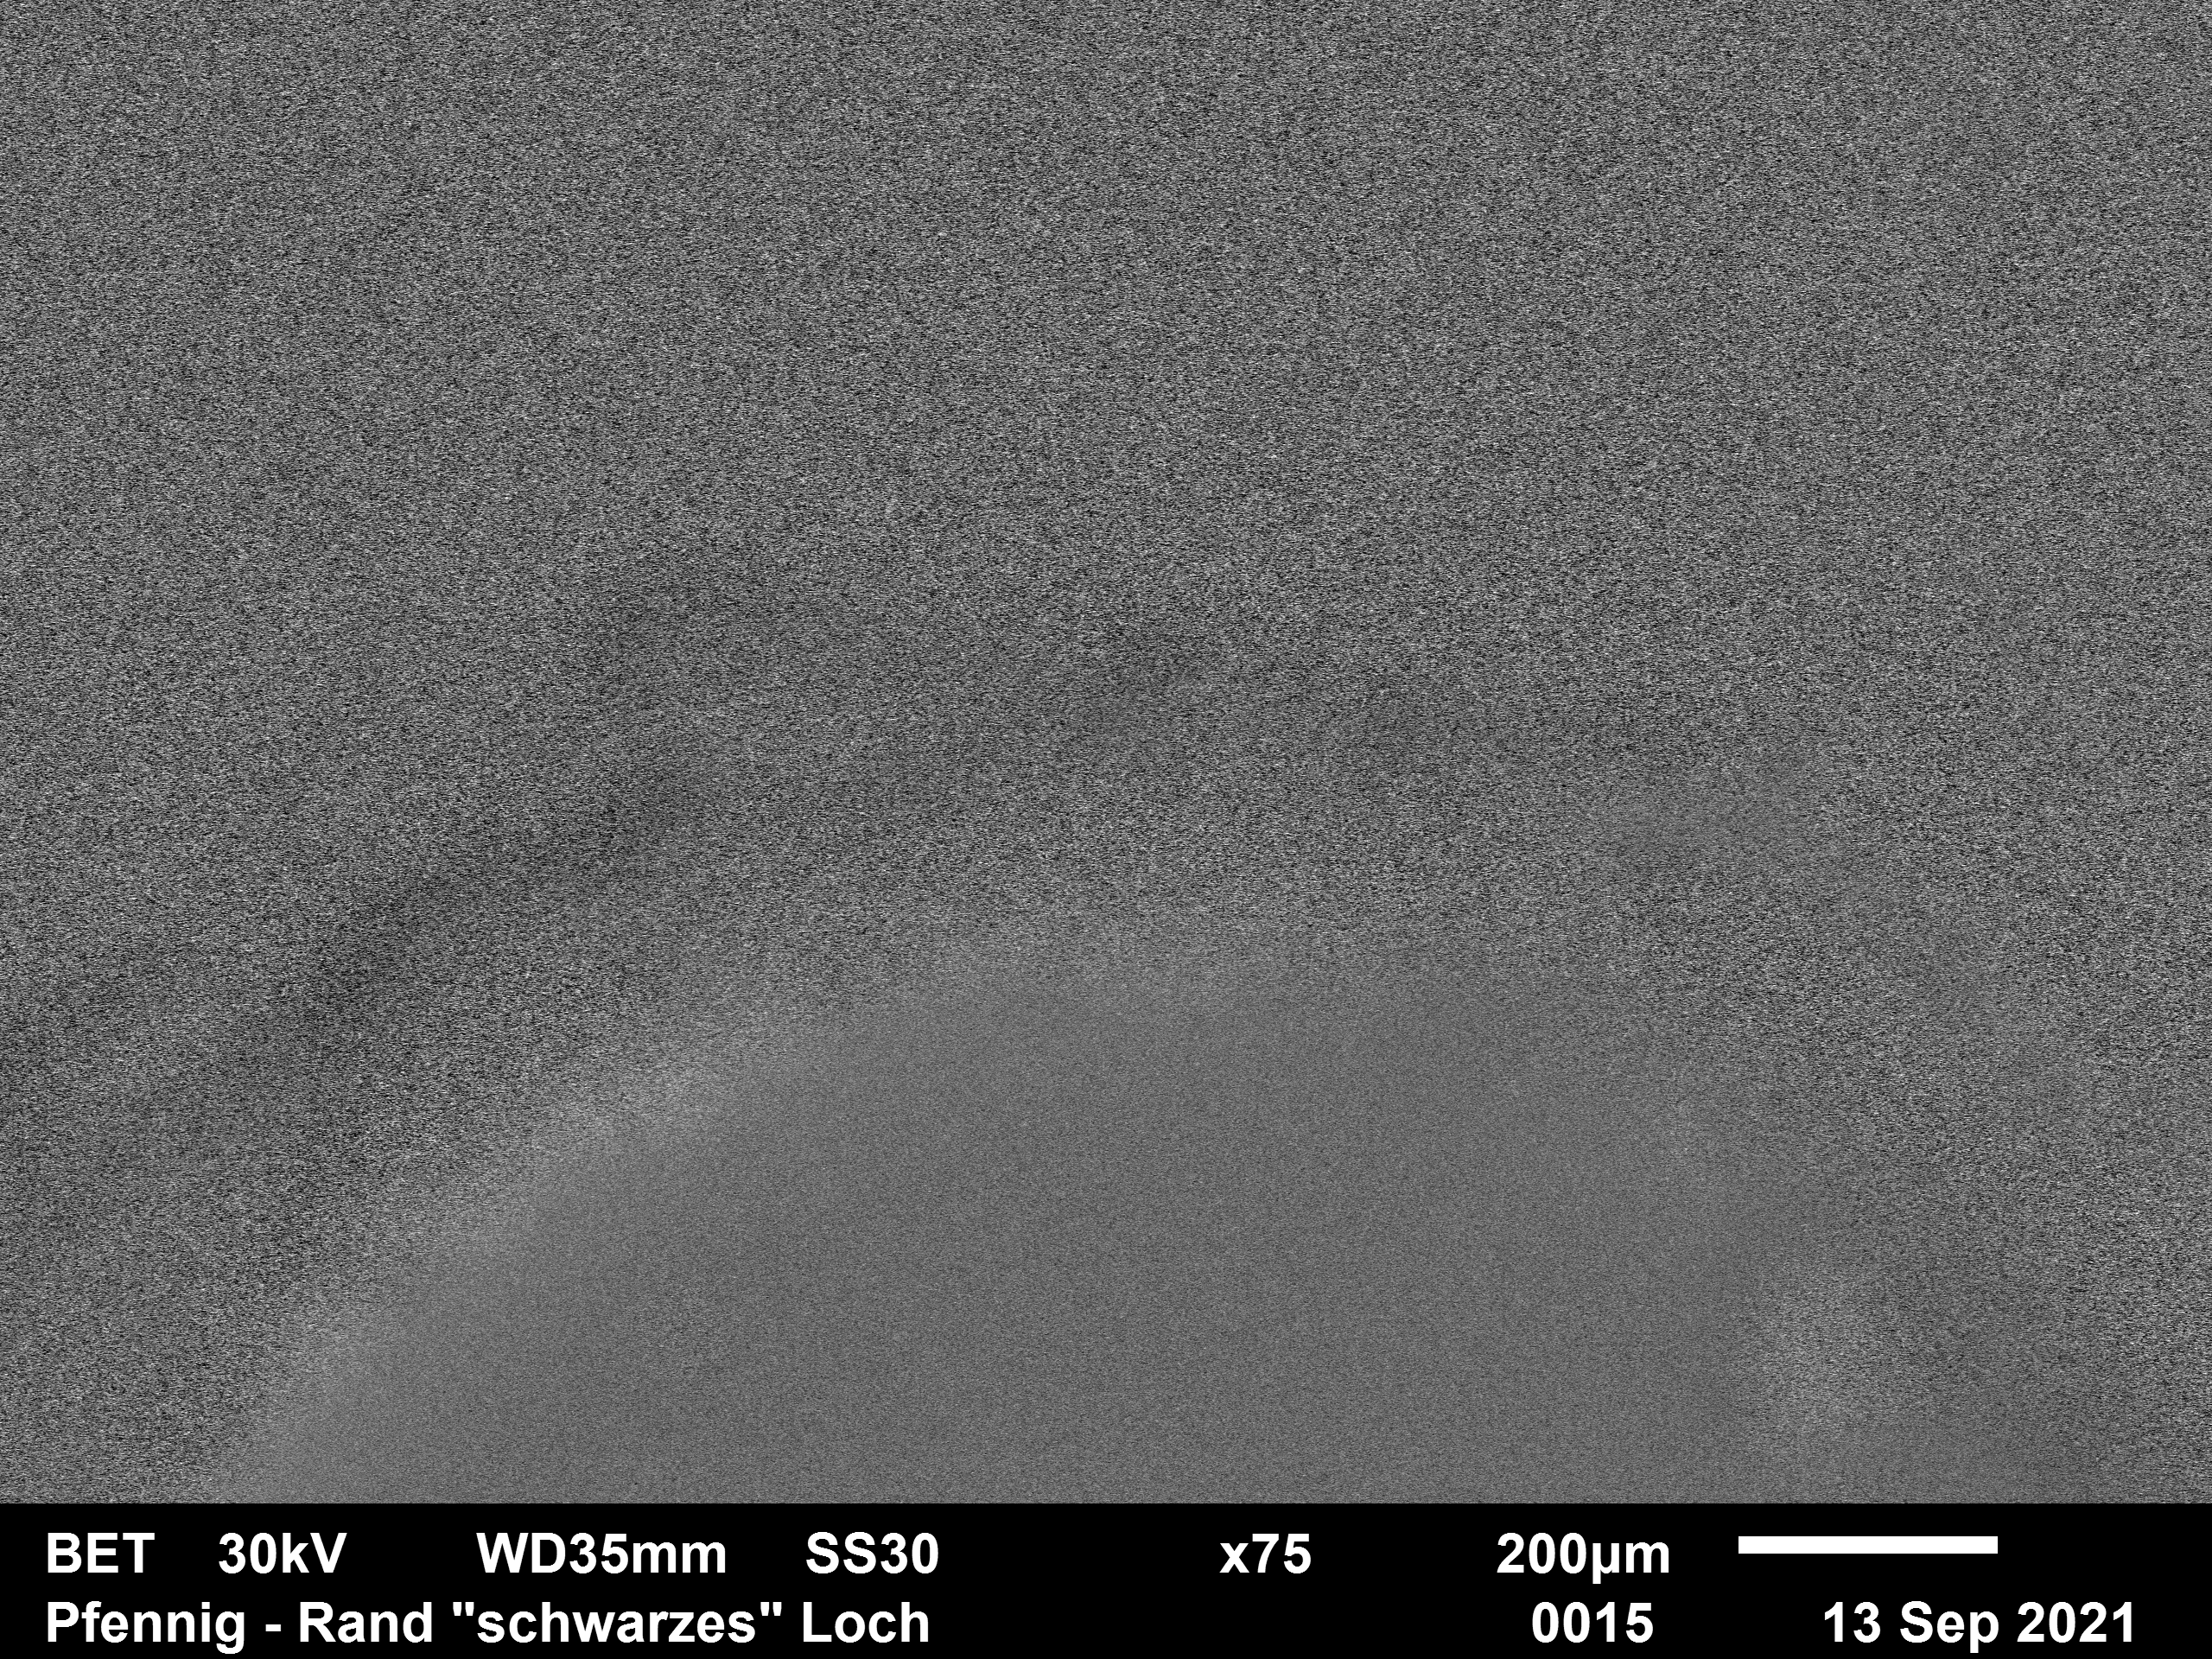
\includegraphics[width=\textwidth]{Auswertung/A/0015.png}
        \caption{$U_B = 30$ kV}
    \end{subfigure}
    
    \caption{BET bei unterschiedlichen Beschleunigunsspannungen}
\end{figure}

Für die Bilder im BET Modus lassen sich wenig Aussagen machen, da die Bildqualität im Allgemeinen sehr schlecht ist. Es lassen sich nur kannten erkennen, was im Topo-Mode keine Überraschung ist. Außerdem liegt die Vermutung nahe, dass die Einstellung des Fokus für $U_B = 30$ kV nicht optimal gewählt wurde.

\newpage
Außerdem wurde eine Stelle, am Rand des gefüllten Lochs, mit verschiedenen Stahldurchmessern aufgenommen.
\begin{figure}[h]
    \centering
    
    \begin{subfigure}[b]{0.45\textwidth}
        \centering
        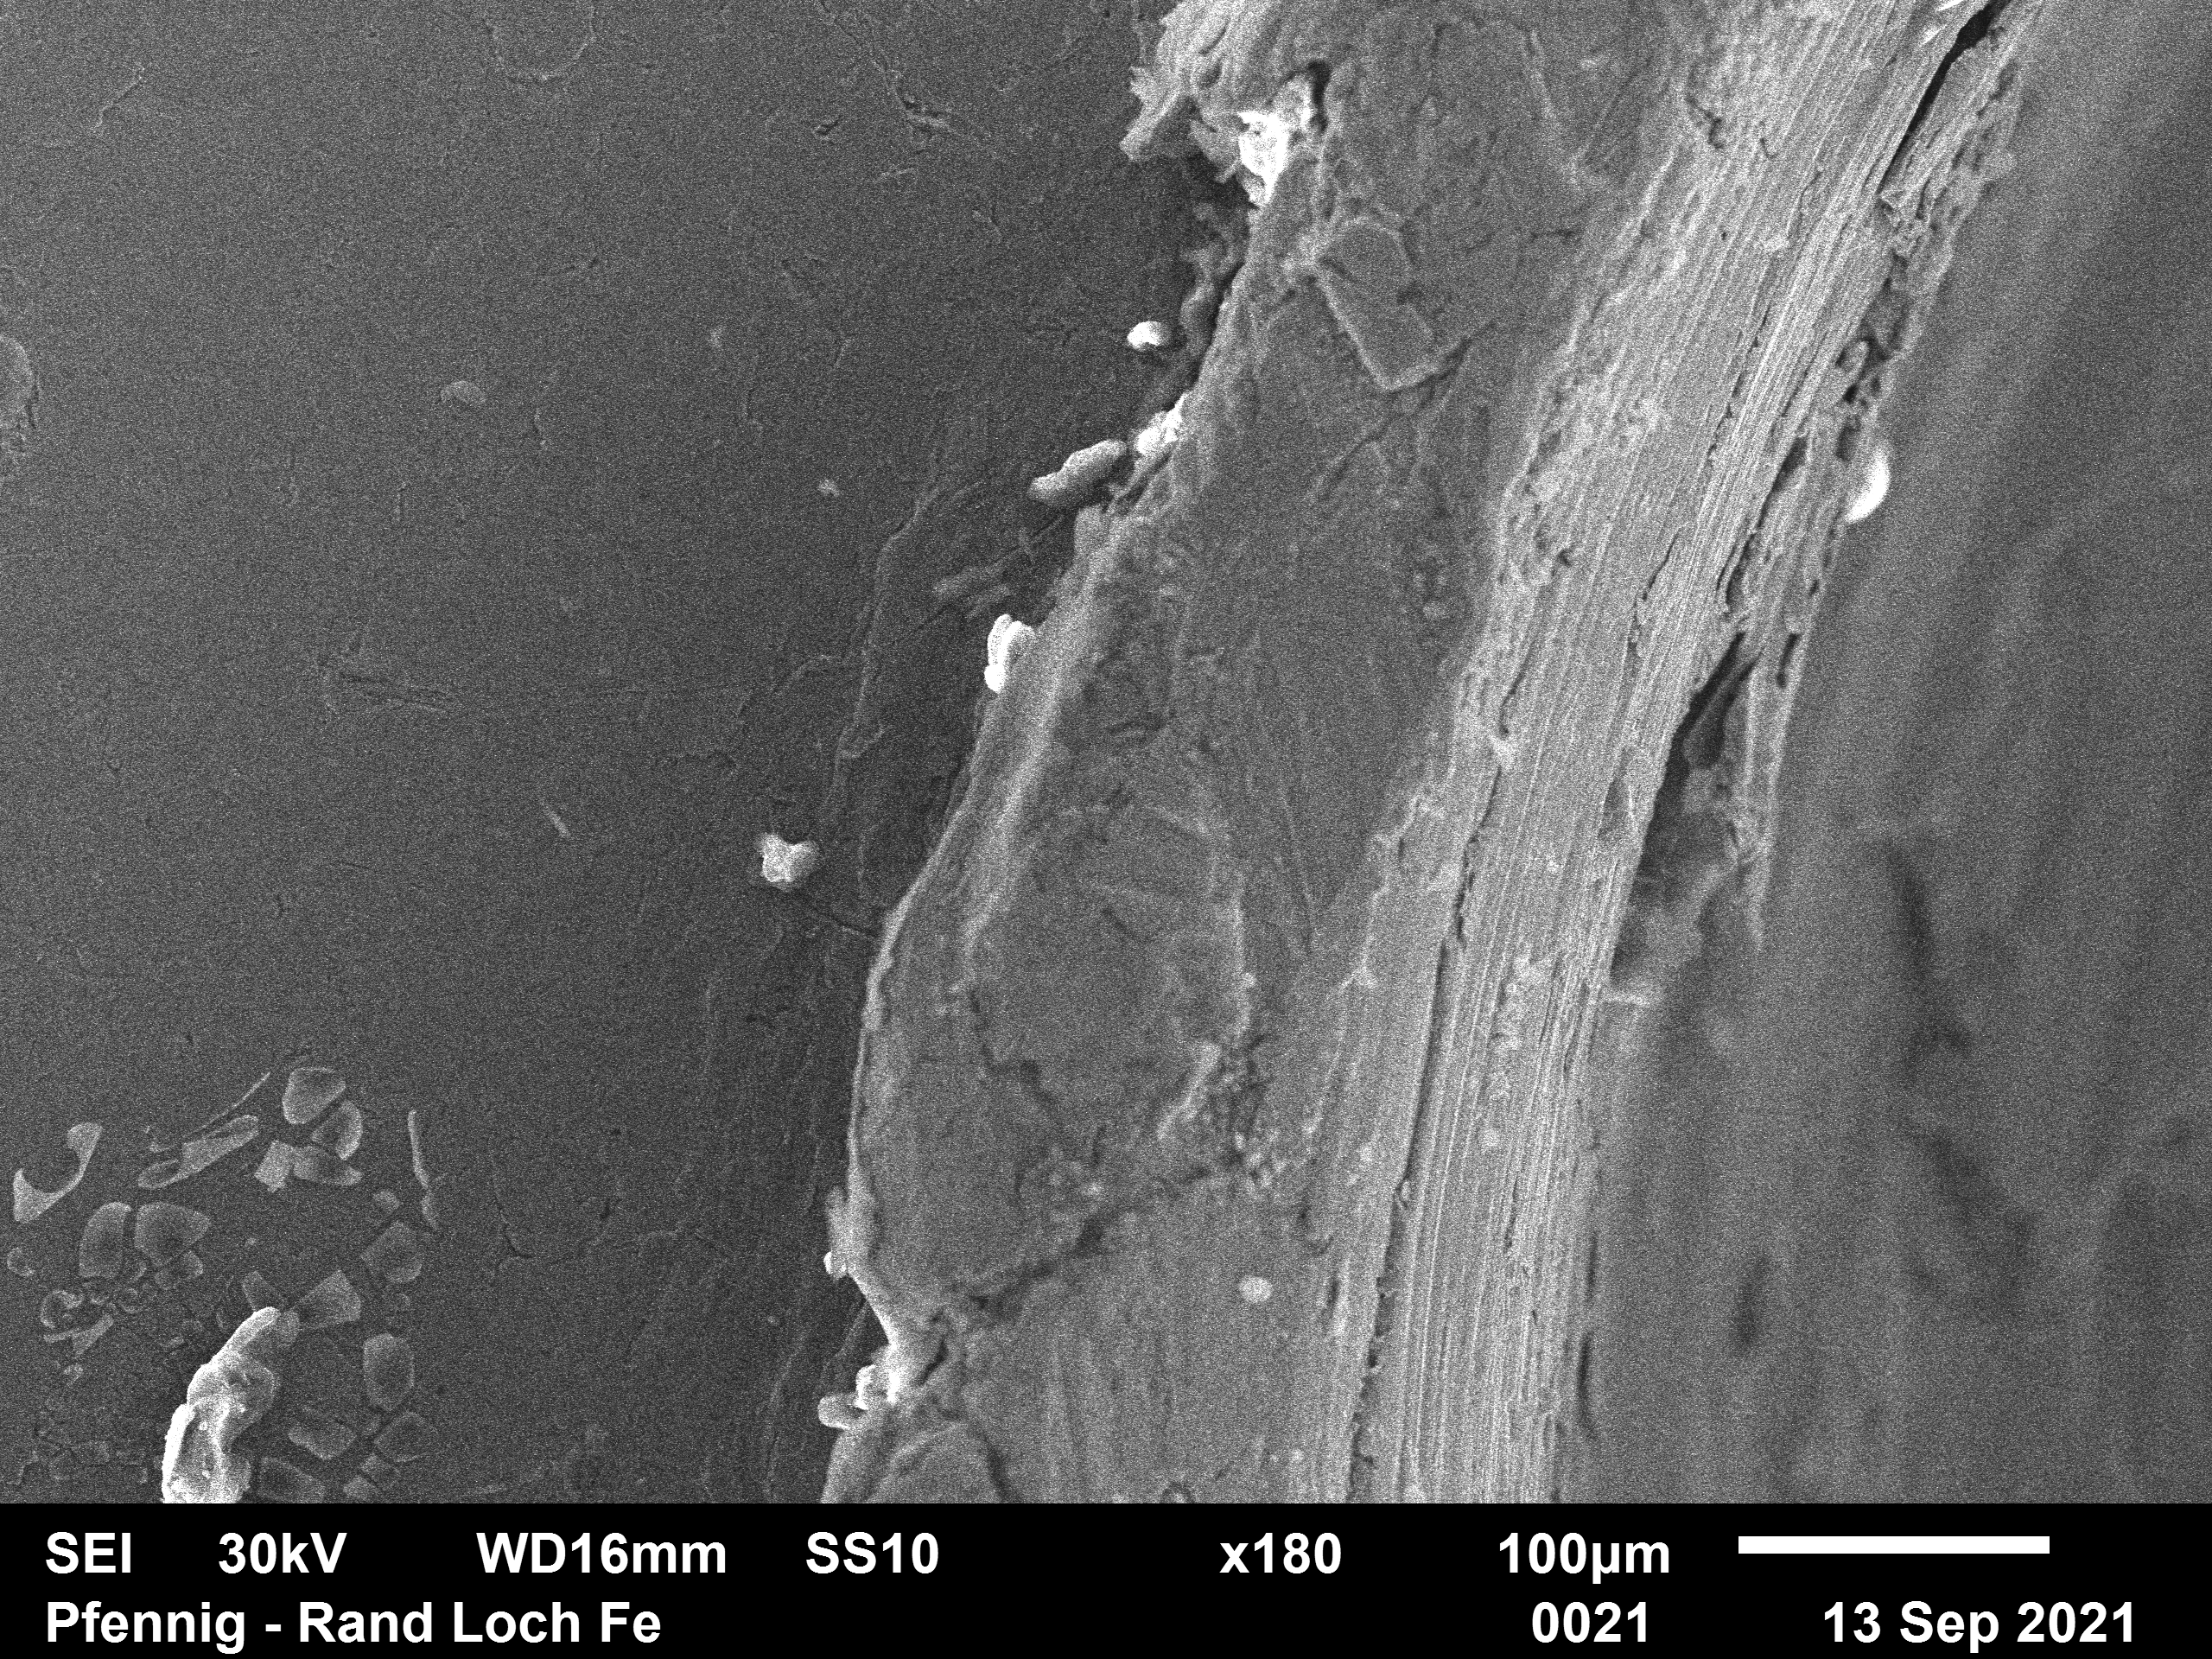
\includegraphics[width=\textwidth]{Auswertung/A/0021.png}
        \caption{SS 10}
    \end{subfigure}
    \hfill
    \begin{subfigure}[b]{0.45\textwidth}
        \centering
        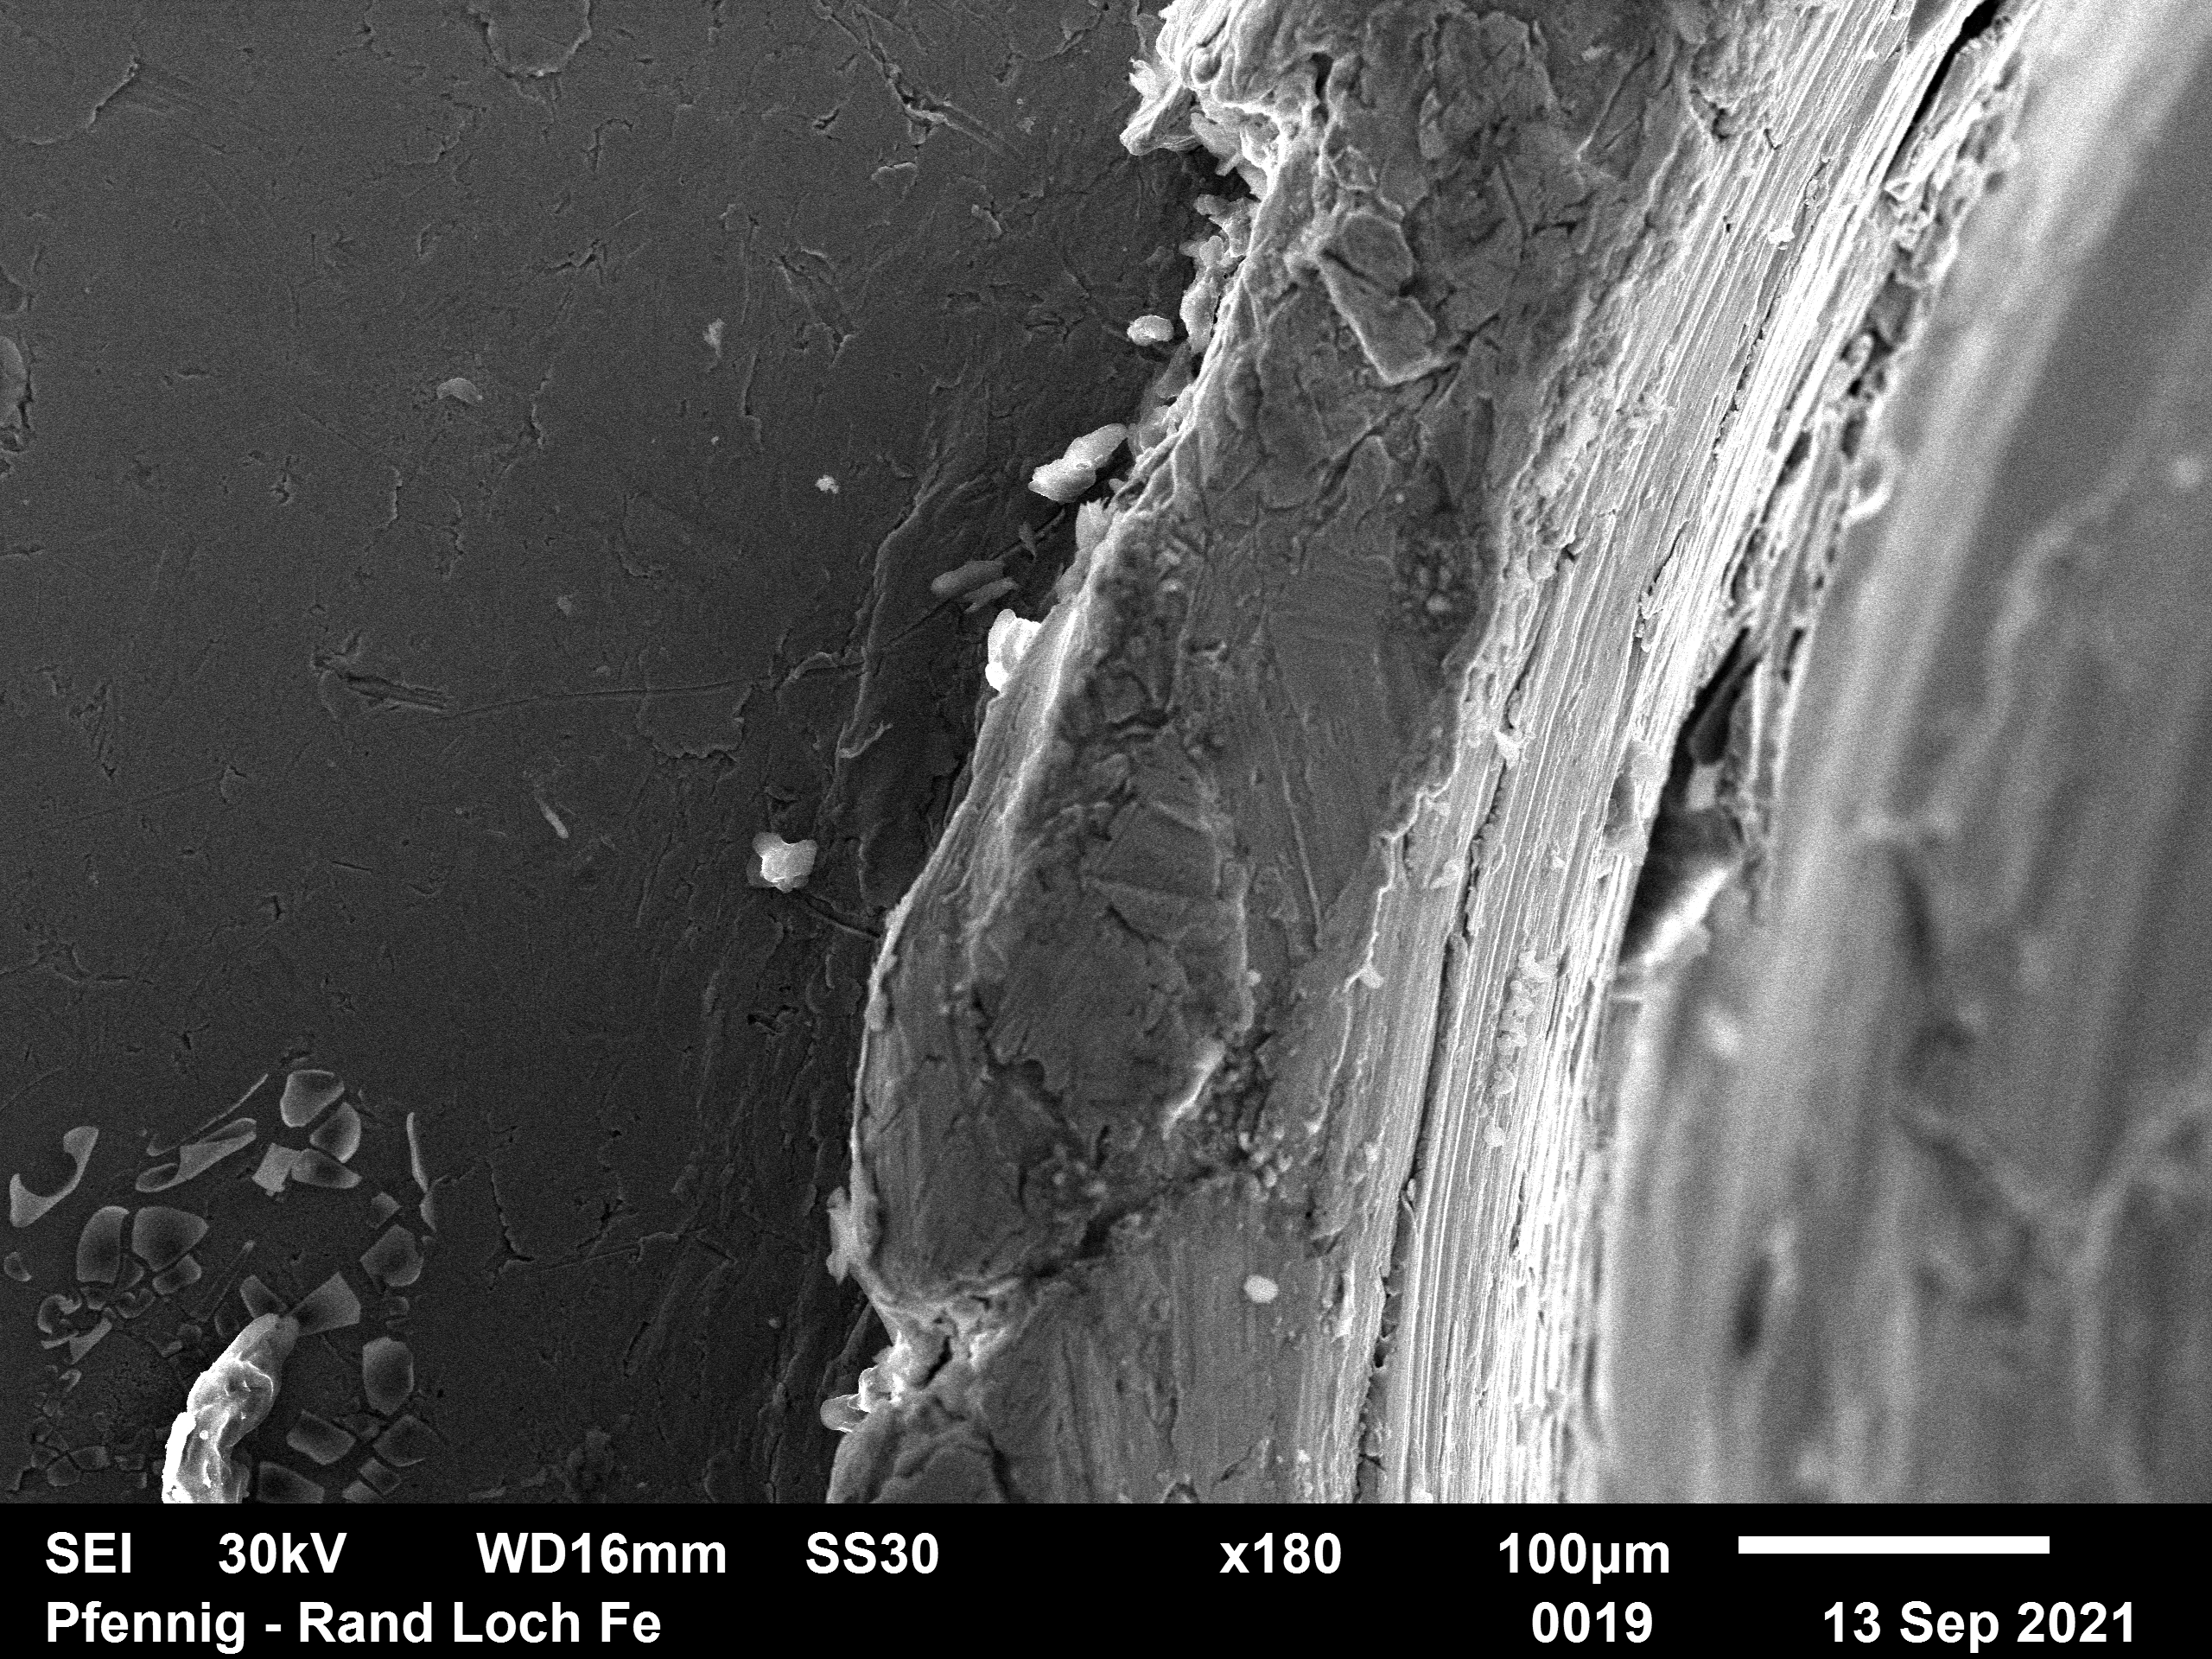
\includegraphics[width=\textwidth]{Auswertung/A/0019.png}
        \caption{SS 30}
    \end{subfigure}
    \\
    \begin{subfigure}[b]{0.45\textwidth}
        \centering
        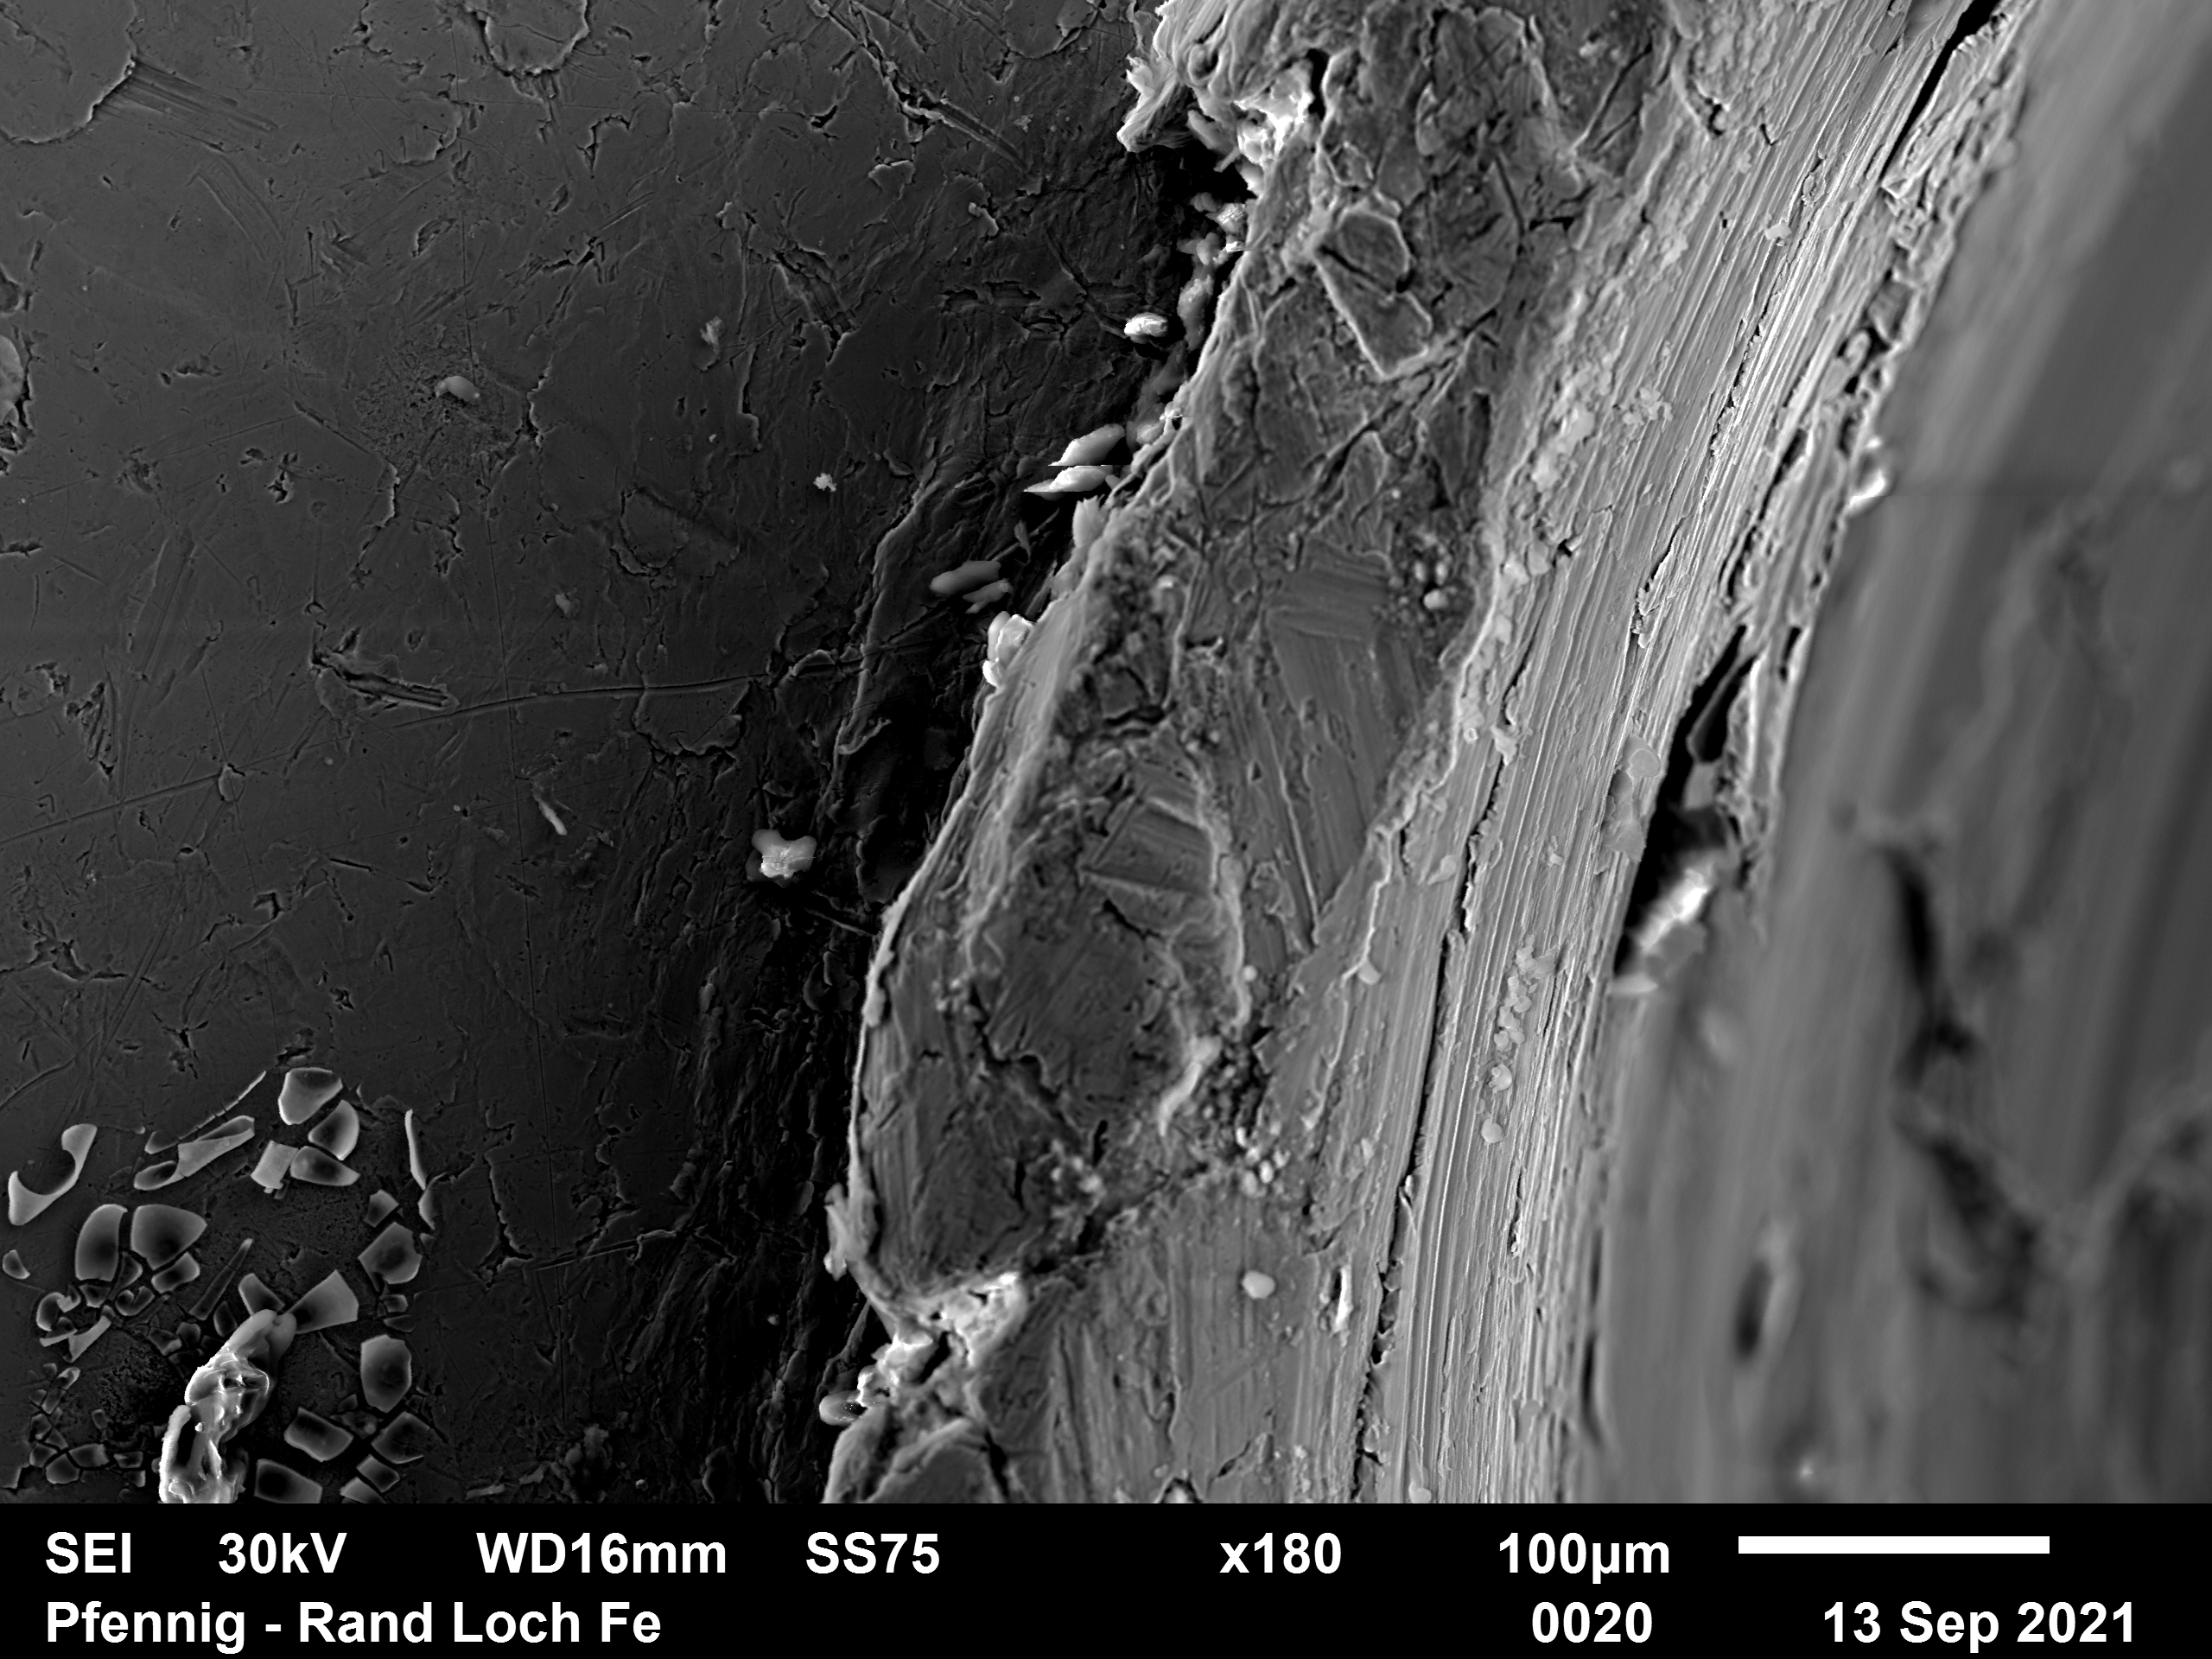
\includegraphics[width=\textwidth]{Auswertung/A/0020.png}
        \caption{SS 75}
    \end{subfigure}
    \caption{SEI bei unterschiedlichen Strahldurschmessern}
\end{figure}

Hier fällt auf, dass die Bilder mit abnehmenden SS körniger werden und somit auch weniger Details zu erkennen sind. Außerdem wird der Kontrast mit zunehmenden SS besser, was aber auch durch unterschiedliche Kontrasteinstellung verursacht werden kann.

\newpage
\subsection*{EDX Analyse}
Nun sollen das Röntgenspektrum der Münze, sowie des andersartigen Lochs mithilfe des EDX Detektors aufgezeichnet werden.Mit dessen Hilfe kann die Materialzusammensetzung ermittelt werden. \\

Zuerst wurde das Spektrum des Grundmaterials der Münze aufgenommen: 
\begin{figure}[h]
    \centering
    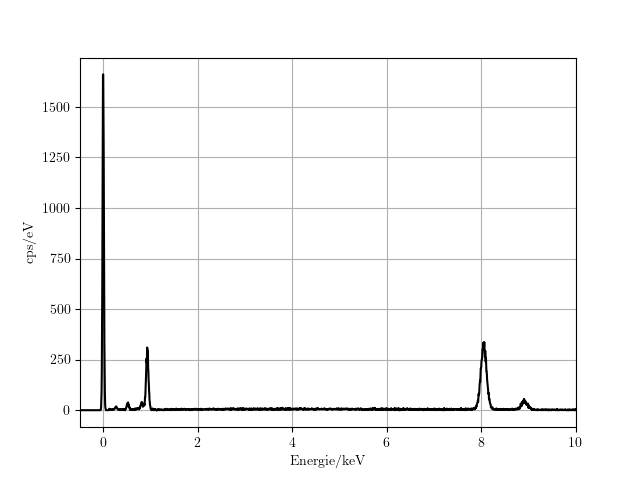
\includegraphics[width=\textwidth]{Auswertung/A/EdxFl.png}
    \caption{Röntgenspektrum der Münze}
\end{figure}

Die EDX Analyse wird weitestgehend automatisch vom Computer übernommen. Nach Aktivierung der Messung wird ein Röntgenspektrum aufgezeichnet. Anhand der Peaks werden die enthaltenen Elemente bestimmt und anhand der Intensität dieser wird die Konzentration der jeweiligen Stoffe durch den PC ermittelt.

\begin{table}[h]
    \centering
    \begin{tabular}{c|c|c|c|c|c|c}
        Element & OZ &Serie& unn. C & norm. C &  Atom. C  & Fehler (1 Sigma) \\
         & & & [Gew. \%] & [Gew. \%] & [At. \%] & [Gew. \%] \\
        \hline\hline
        C & 6 & K & 13,96&11,87&23,84 & 35,27\\
        O & 8 & K & 10,72&9,11&20,33 & 3,41\\
        Cu & 29 & K & 92,94&79,02&44,40 & 2,50\\
    \end{tabular}
    \caption{Ergebnisse der EDX-Analyse der Münze}
\end{table}

Nach der Analyse geht klar hervor das Kupfer den größten Anteil ausmacht, was bei einer Kupfermünze alles andere als verwunderlich ist. Die Übrigen Bestandteile, Kohlenstoff und Sauerstoff, sind wohl auf organische Verunreinigungen zurückzuführen.

\newpage
Anschließend wurde das Spektrum des Materials in dem hellen Loch aufgenommen: 
\begin{figure}[h]
    \centering
    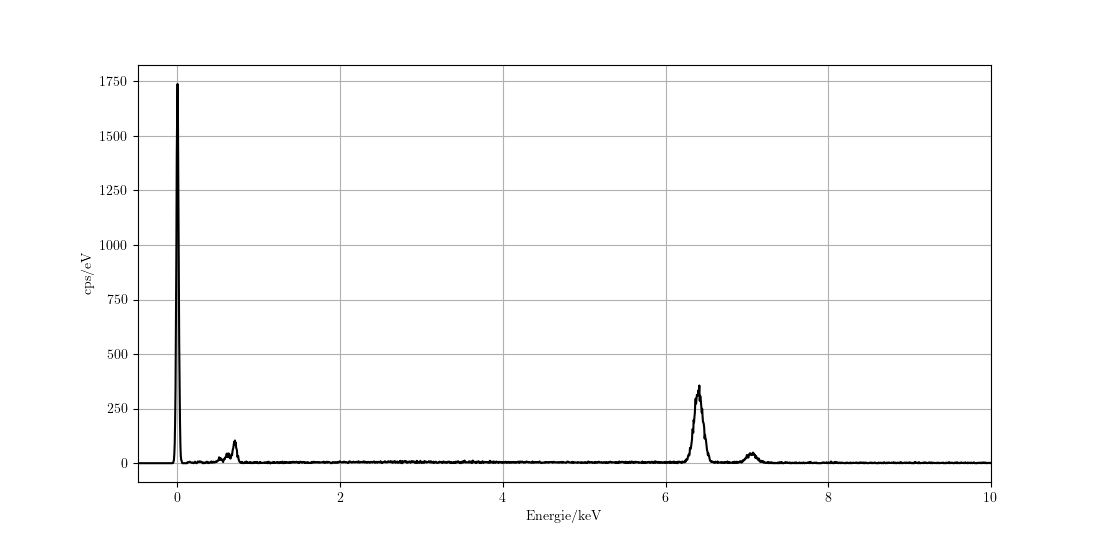
\includegraphics[width=\textwidth]{Auswertung/A/EdxLoch.png}
    \caption{Röntgenspektrum des hellen Lochs}
\end{figure}


\begin{table}[h]
    \centering
    \begin{tabular}{c|c|c|c|c|c|c}
        Element & OZ &Serie& unn. C & norm. C &  Atom. C  & Fehler (1 Sigma) \\
         & & & [Gew. \%] & [Gew. \%] & [At. \%] & [Gew. \%] \\
        \hline\hline
        C & 6 & K & 7,06&7,57&23,84 & 4,17\\
        O & 8 & K & 7,52&8,06&19,05 & 2,83\\
        Fe & 26 & K & 78,68&84,36&57,11 & 2,19\\
    \end{tabular}
    \caption{Ergebnisse der EDX-Analyse des hellen Lochs}
\end{table}

Das Ergebnis der Zweiten EDX Analyse zeigt hingegen, dass das helle Loch neben den organischen Verunreinigungen vor allem Eisen enthält. Was nahelegt, dass dieses Loch mit Eisen gefüllt worden ist.

\newpage
\section{Fliege}

Als nächste Probe wurde eine Fliege untersucht. Da es sich hierbei um organisches Material handelt, wurde sie mit Gold bedampft, um eine Untersuchung möglich zu machen. Weiterhin ist darauf zu achten, die Beschleunigungsspannung nicht zu groß (ca. 10  kV) einzustellen, da die Probe sonst beschädigt werden kann. \\

Zuerst wurde die Fliege im Ganzen aufgenommen. Um dabei eine höhere Tiefenschärfe zu erreichen wurde ein großer Arbeitsabstand eingestellt.
\begin{figure}[h]
    \centering
    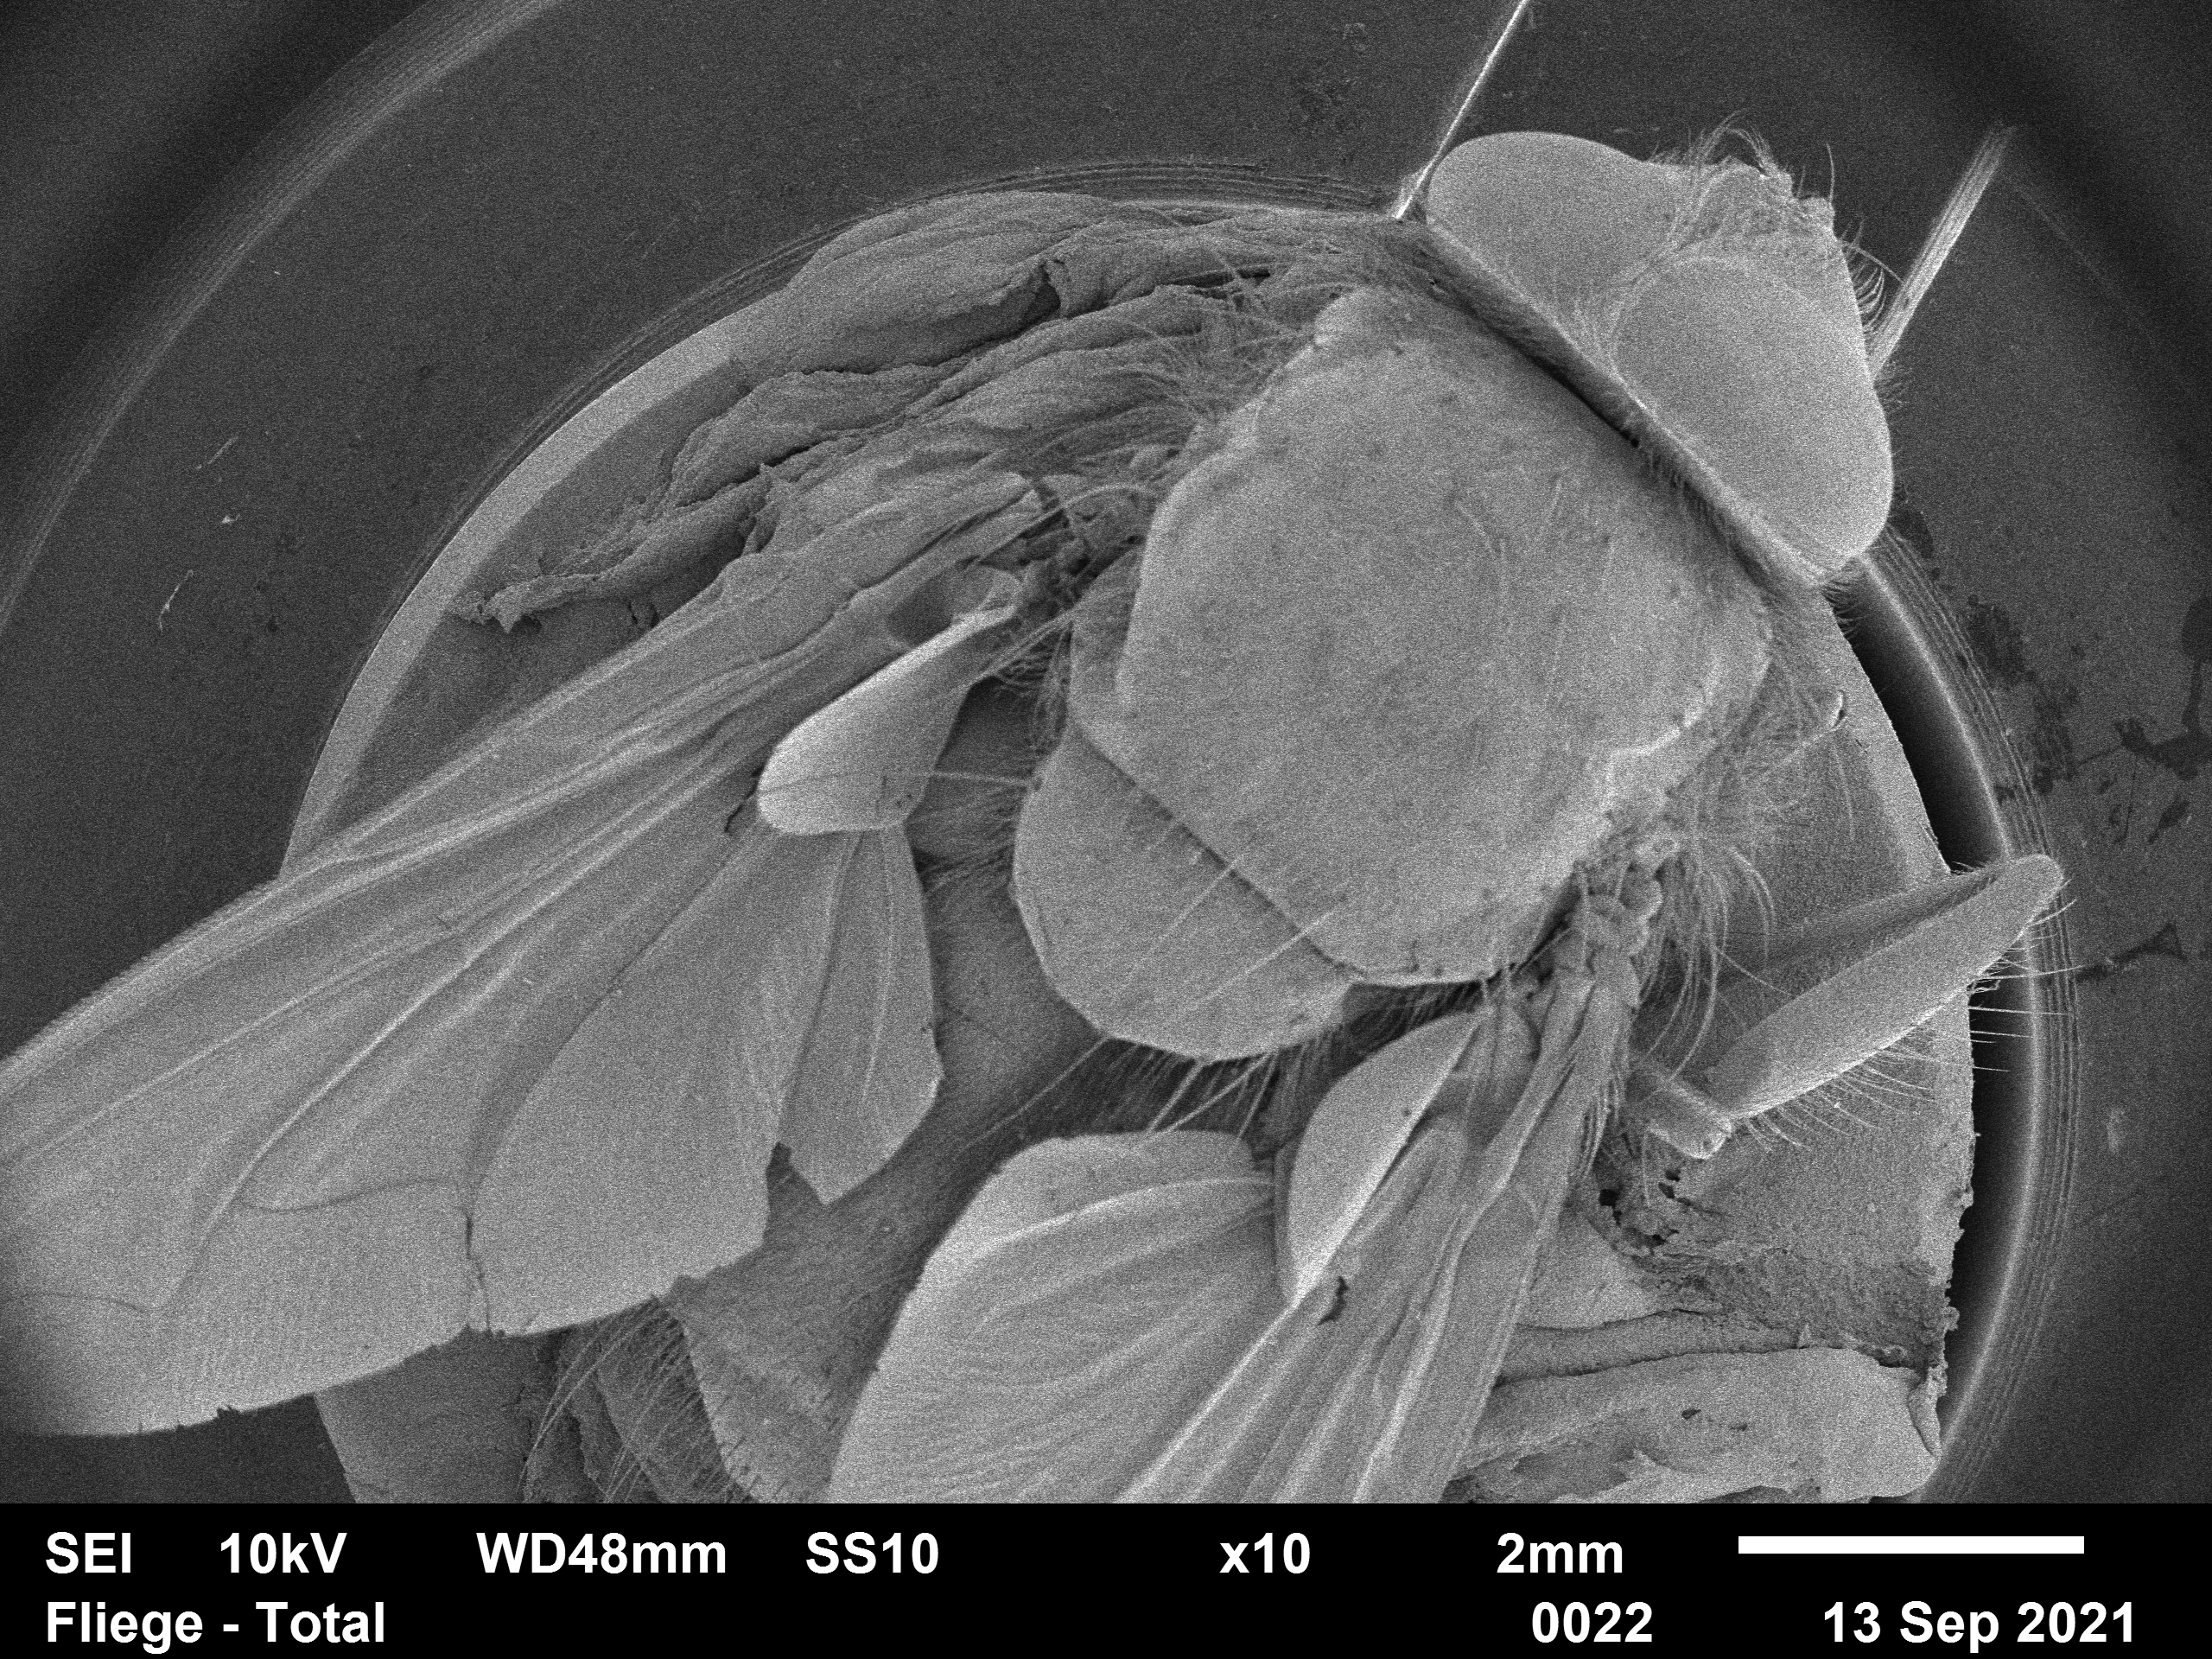
\includegraphics[width=\textwidth]{Auswertung/B/0022.png}
    \caption{Gesamtaufnahme der Fliege}
    \label{fig:FGA}
\end{figure}

\newpage
Als Nächstes wurde ein Segment des Facettenauges vermessen, hierfür wurde die Augen der Fliege (in Abbildung \ref{fig:FGA} rechts oben) genauer betrachtet.
\begin{figure}[h]
    \centering
    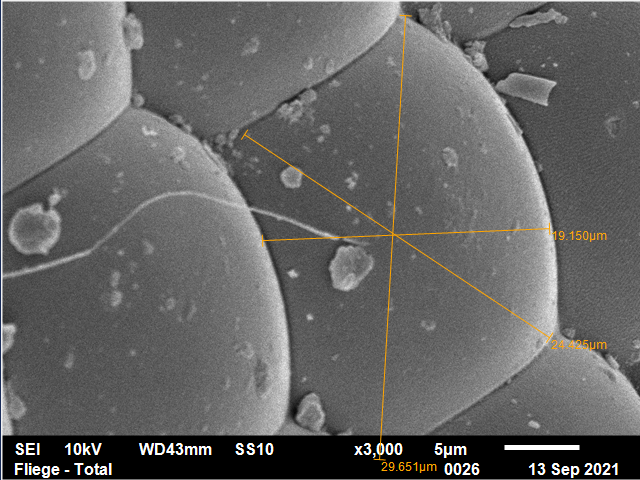
\includegraphics[width=\textwidth]{Auswertung/B/26-2.PNG}
    \caption{Segment eines Facettenauges der Fliege mit Bemaßung}
    \label{fig:FAF}
\end{figure}
In Abbildung \ref{fig:FAF} ist ein Segment des Fliegenauges und die Maßlinien, welche mit dem Vermessungstool der REM Software erzeugt wurden, zu erkennen. Die Körnen die auf der Oberfläche zu erkennen sind, sind Verunreinigungen wie z.B. Staubkörner.\\
Der Durchschnitt der Maßangaben beträgt 24,41 $\mu$m.

\newpage
\section{Zinnstandart}
In diesem Abschnitt sollen der Einfluss des Strahldurchmessers, der Beschleunigungsspannung und des Arbeitsabstands genauer beleuchtet werden. \\

Zuerst wird dazu der Strahldurchmesser variiert.
\begin{figure}[h]
    \centering
    \begin{subfigure}[b]{0.45\textwidth}
        \centering
        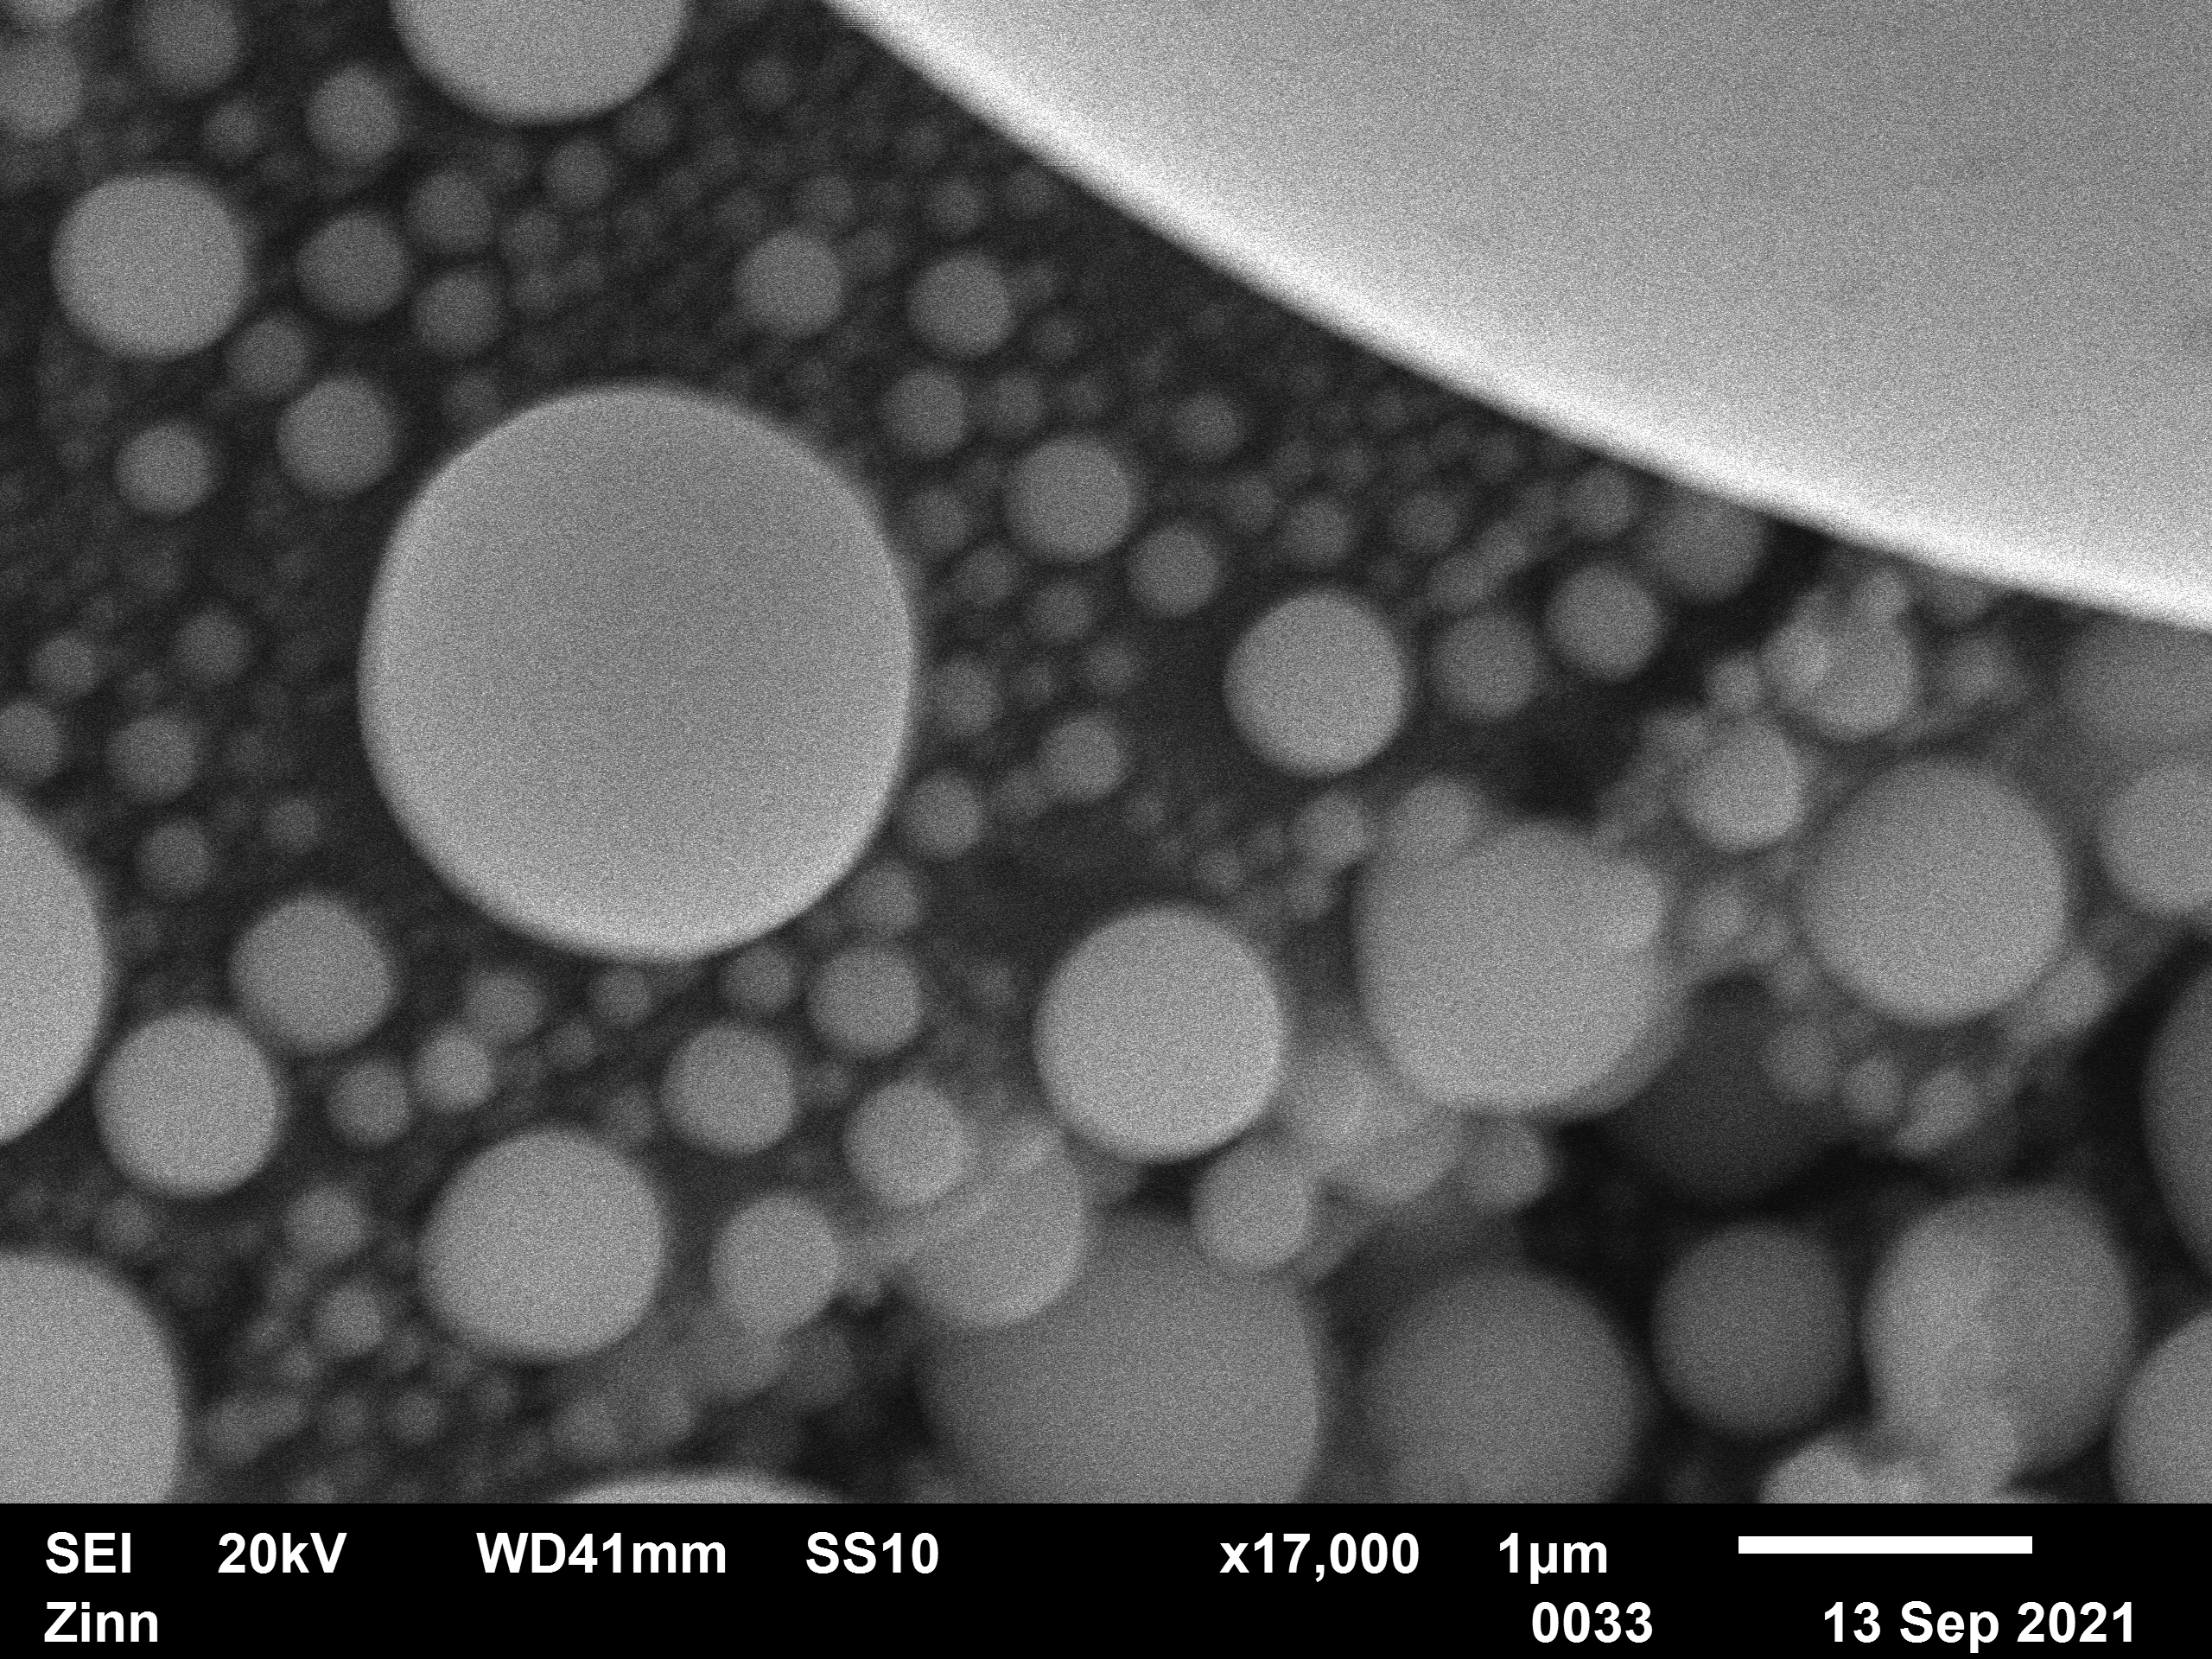
\includegraphics[width=\textwidth]{Auswertung/C/0033.png}
        \caption{SS 10}
    \end{subfigure}
    \hfill
    \begin{subfigure}[b]{0.45\textwidth}
        \centering
        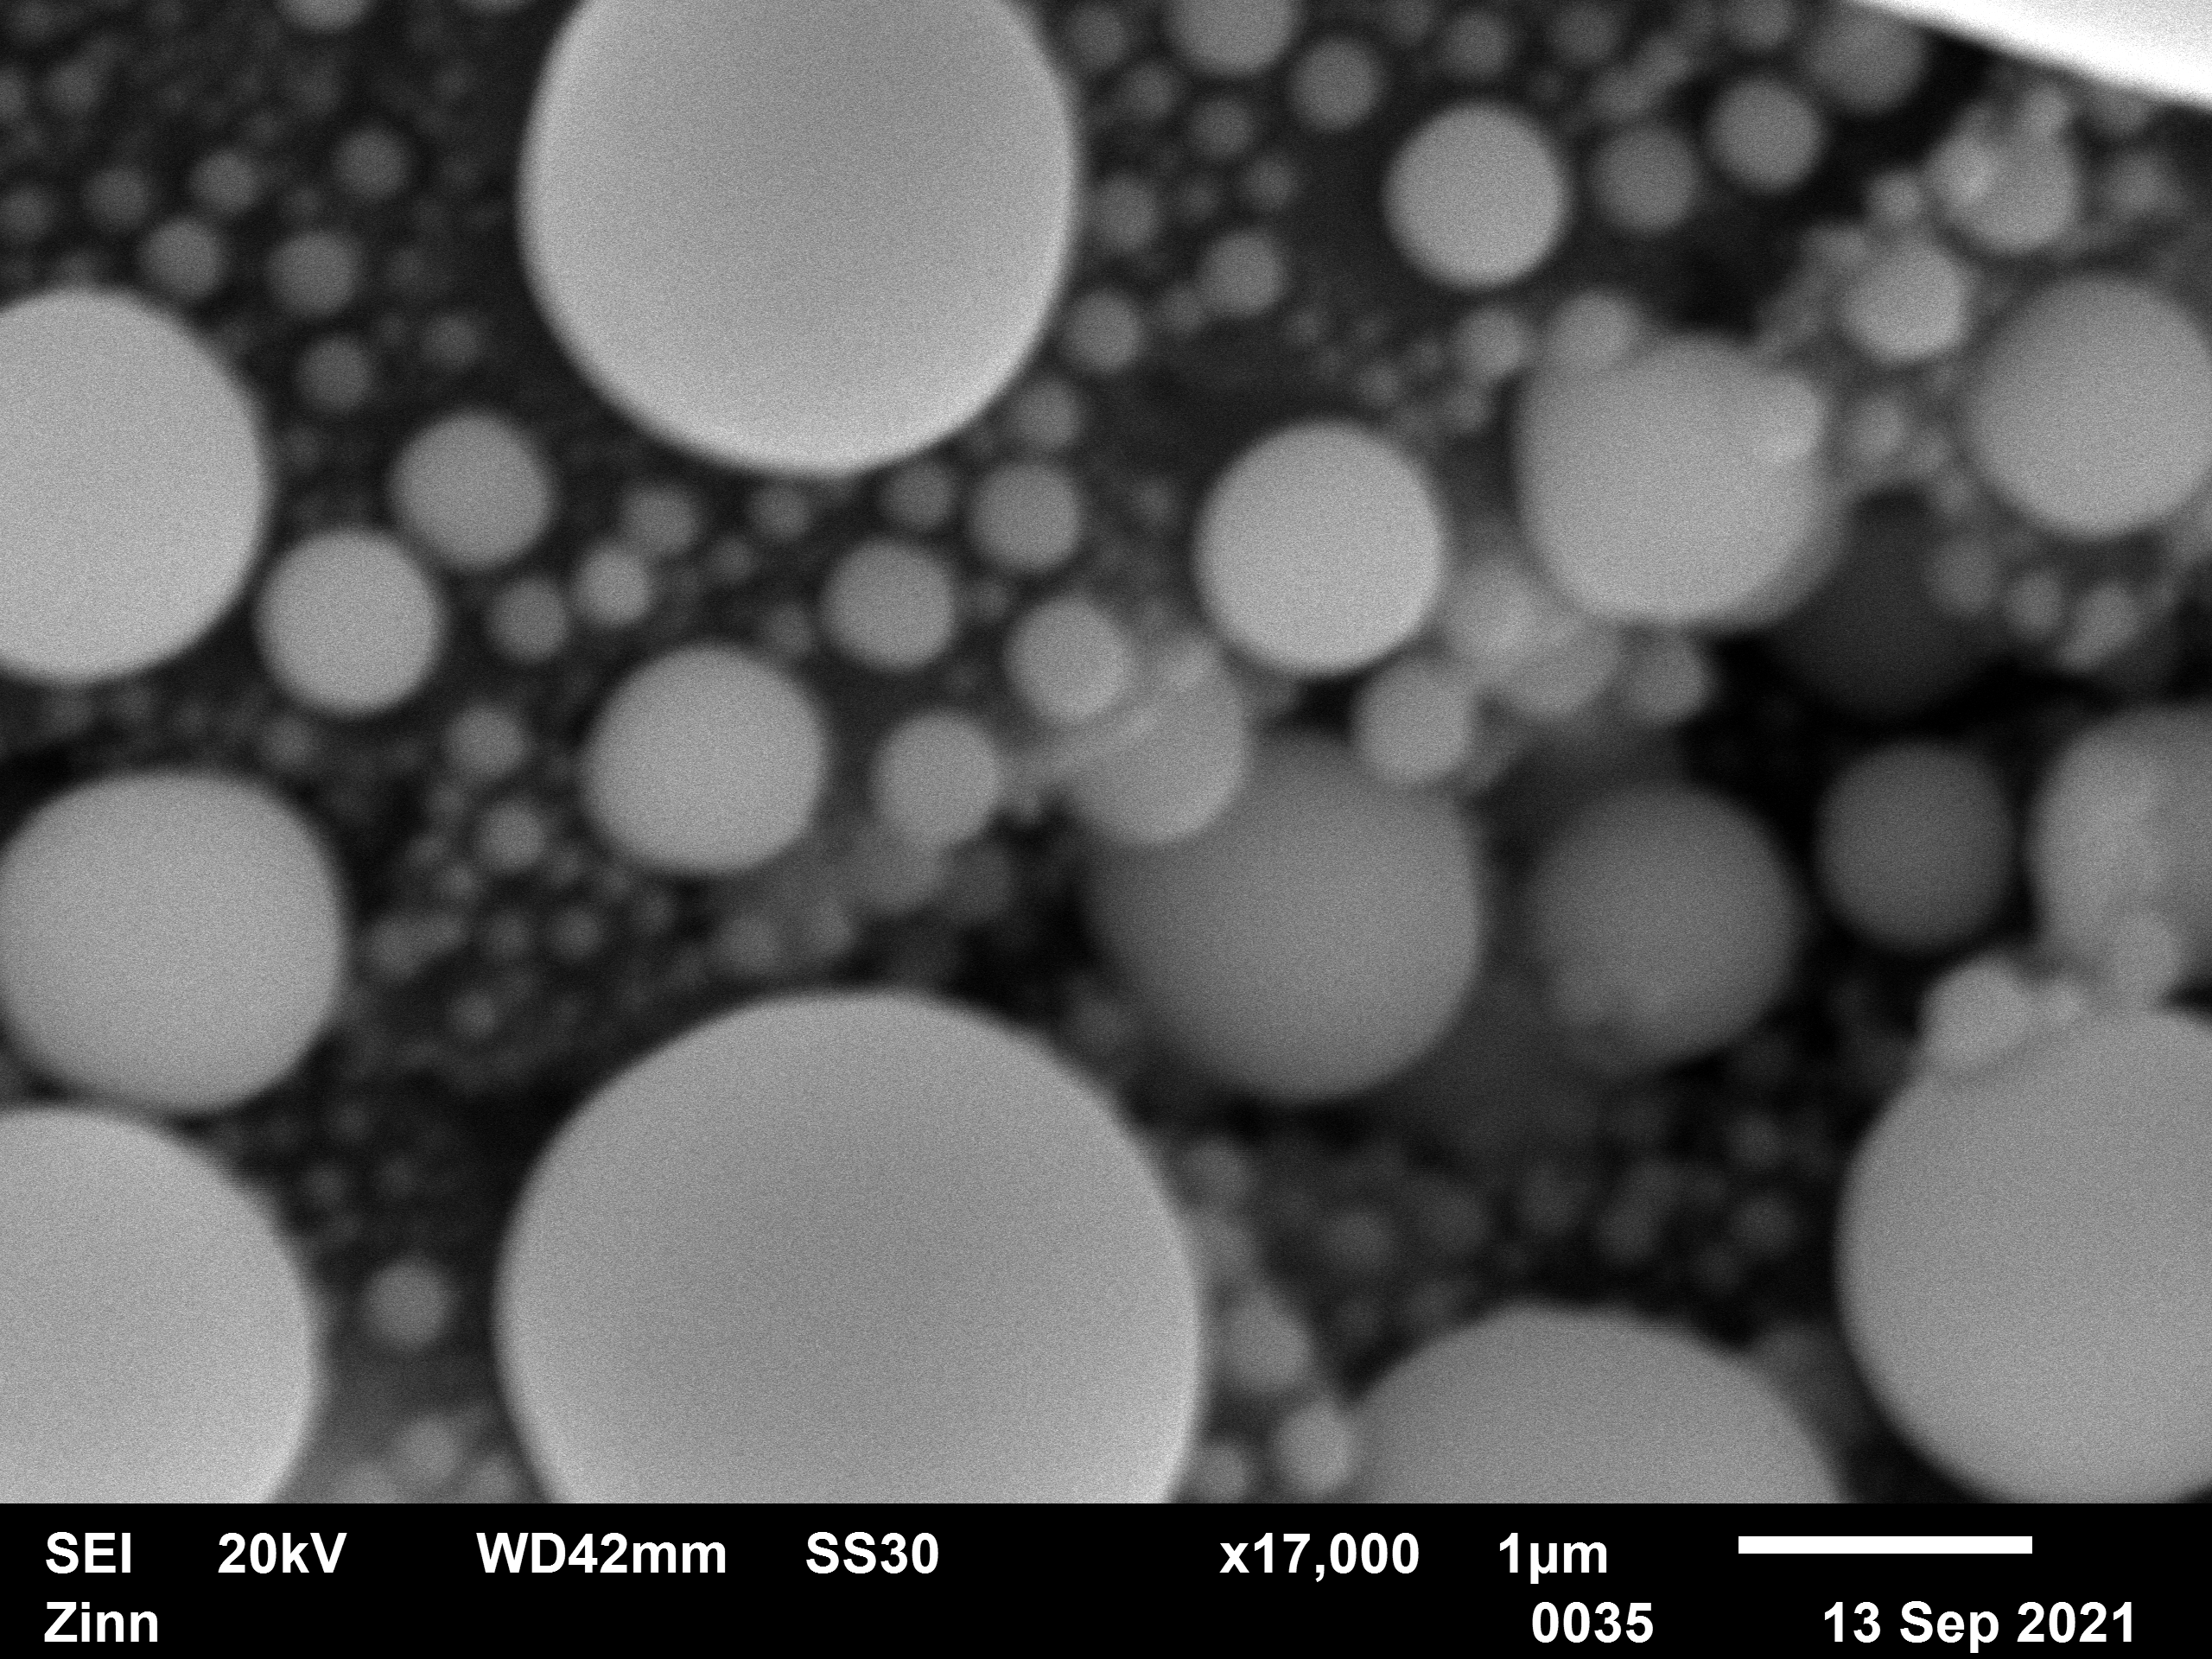
\includegraphics[width=\textwidth]{Auswertung/C/0035.png}
        \caption{SS 30}
    \end{subfigure}
    \\
    \begin{subfigure}[b]{0.45\textwidth}
        \centering
        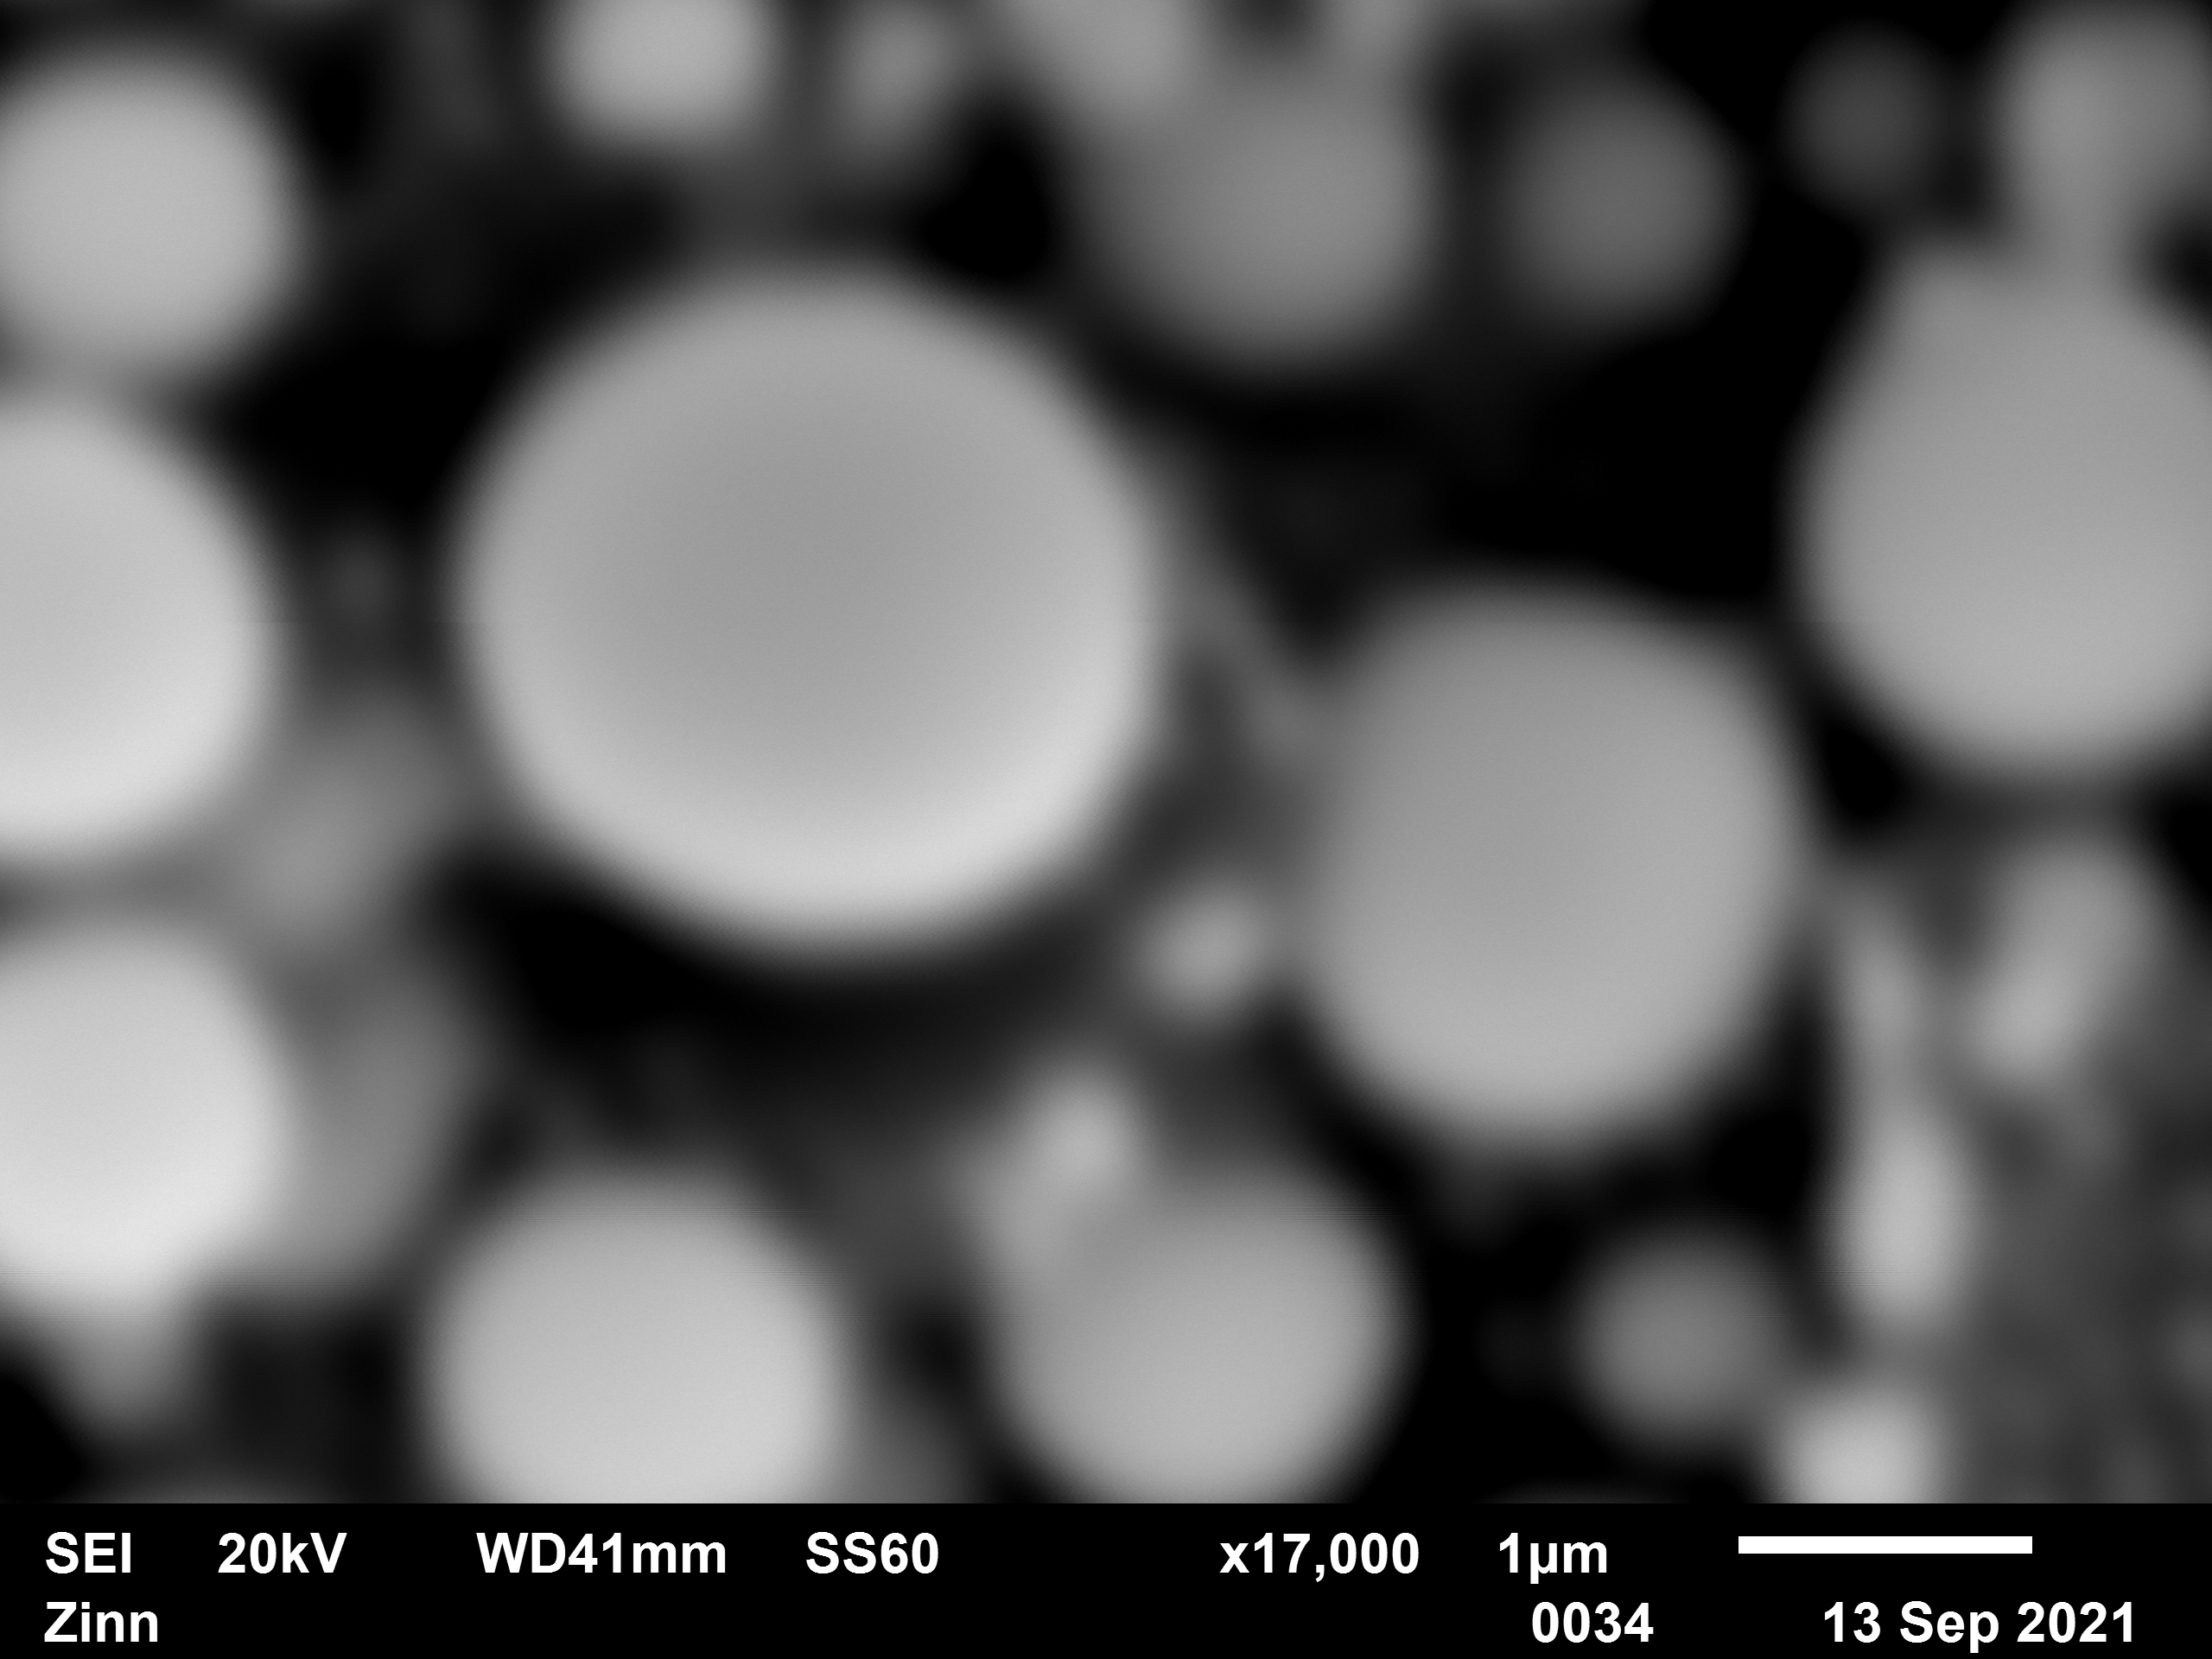
\includegraphics[width=\textwidth]{Auswertung/C/0034.png}
        \caption{SS 60}
    \end{subfigure}
    \caption{Zinstandart bei verschiedenen Strahldurchmessern}
\end{figure}

Es fällt auf, dass mit größerem SS die Schärfe und die Auflösung der Aufnahmen schlechter wurden. Es ist jedoch nicht der wirklich der gleiche Bildausschnitt zu erkennen, die Veränderungen sind aber deutlich unabhängig davon zu erkennen.

\newpage
Außerdem wird auch die Beschleunigungsspannung variiert.
\begin{figure}[h]
    \centering
    \begin{subfigure}[b]{0.45\textwidth}
        \centering
        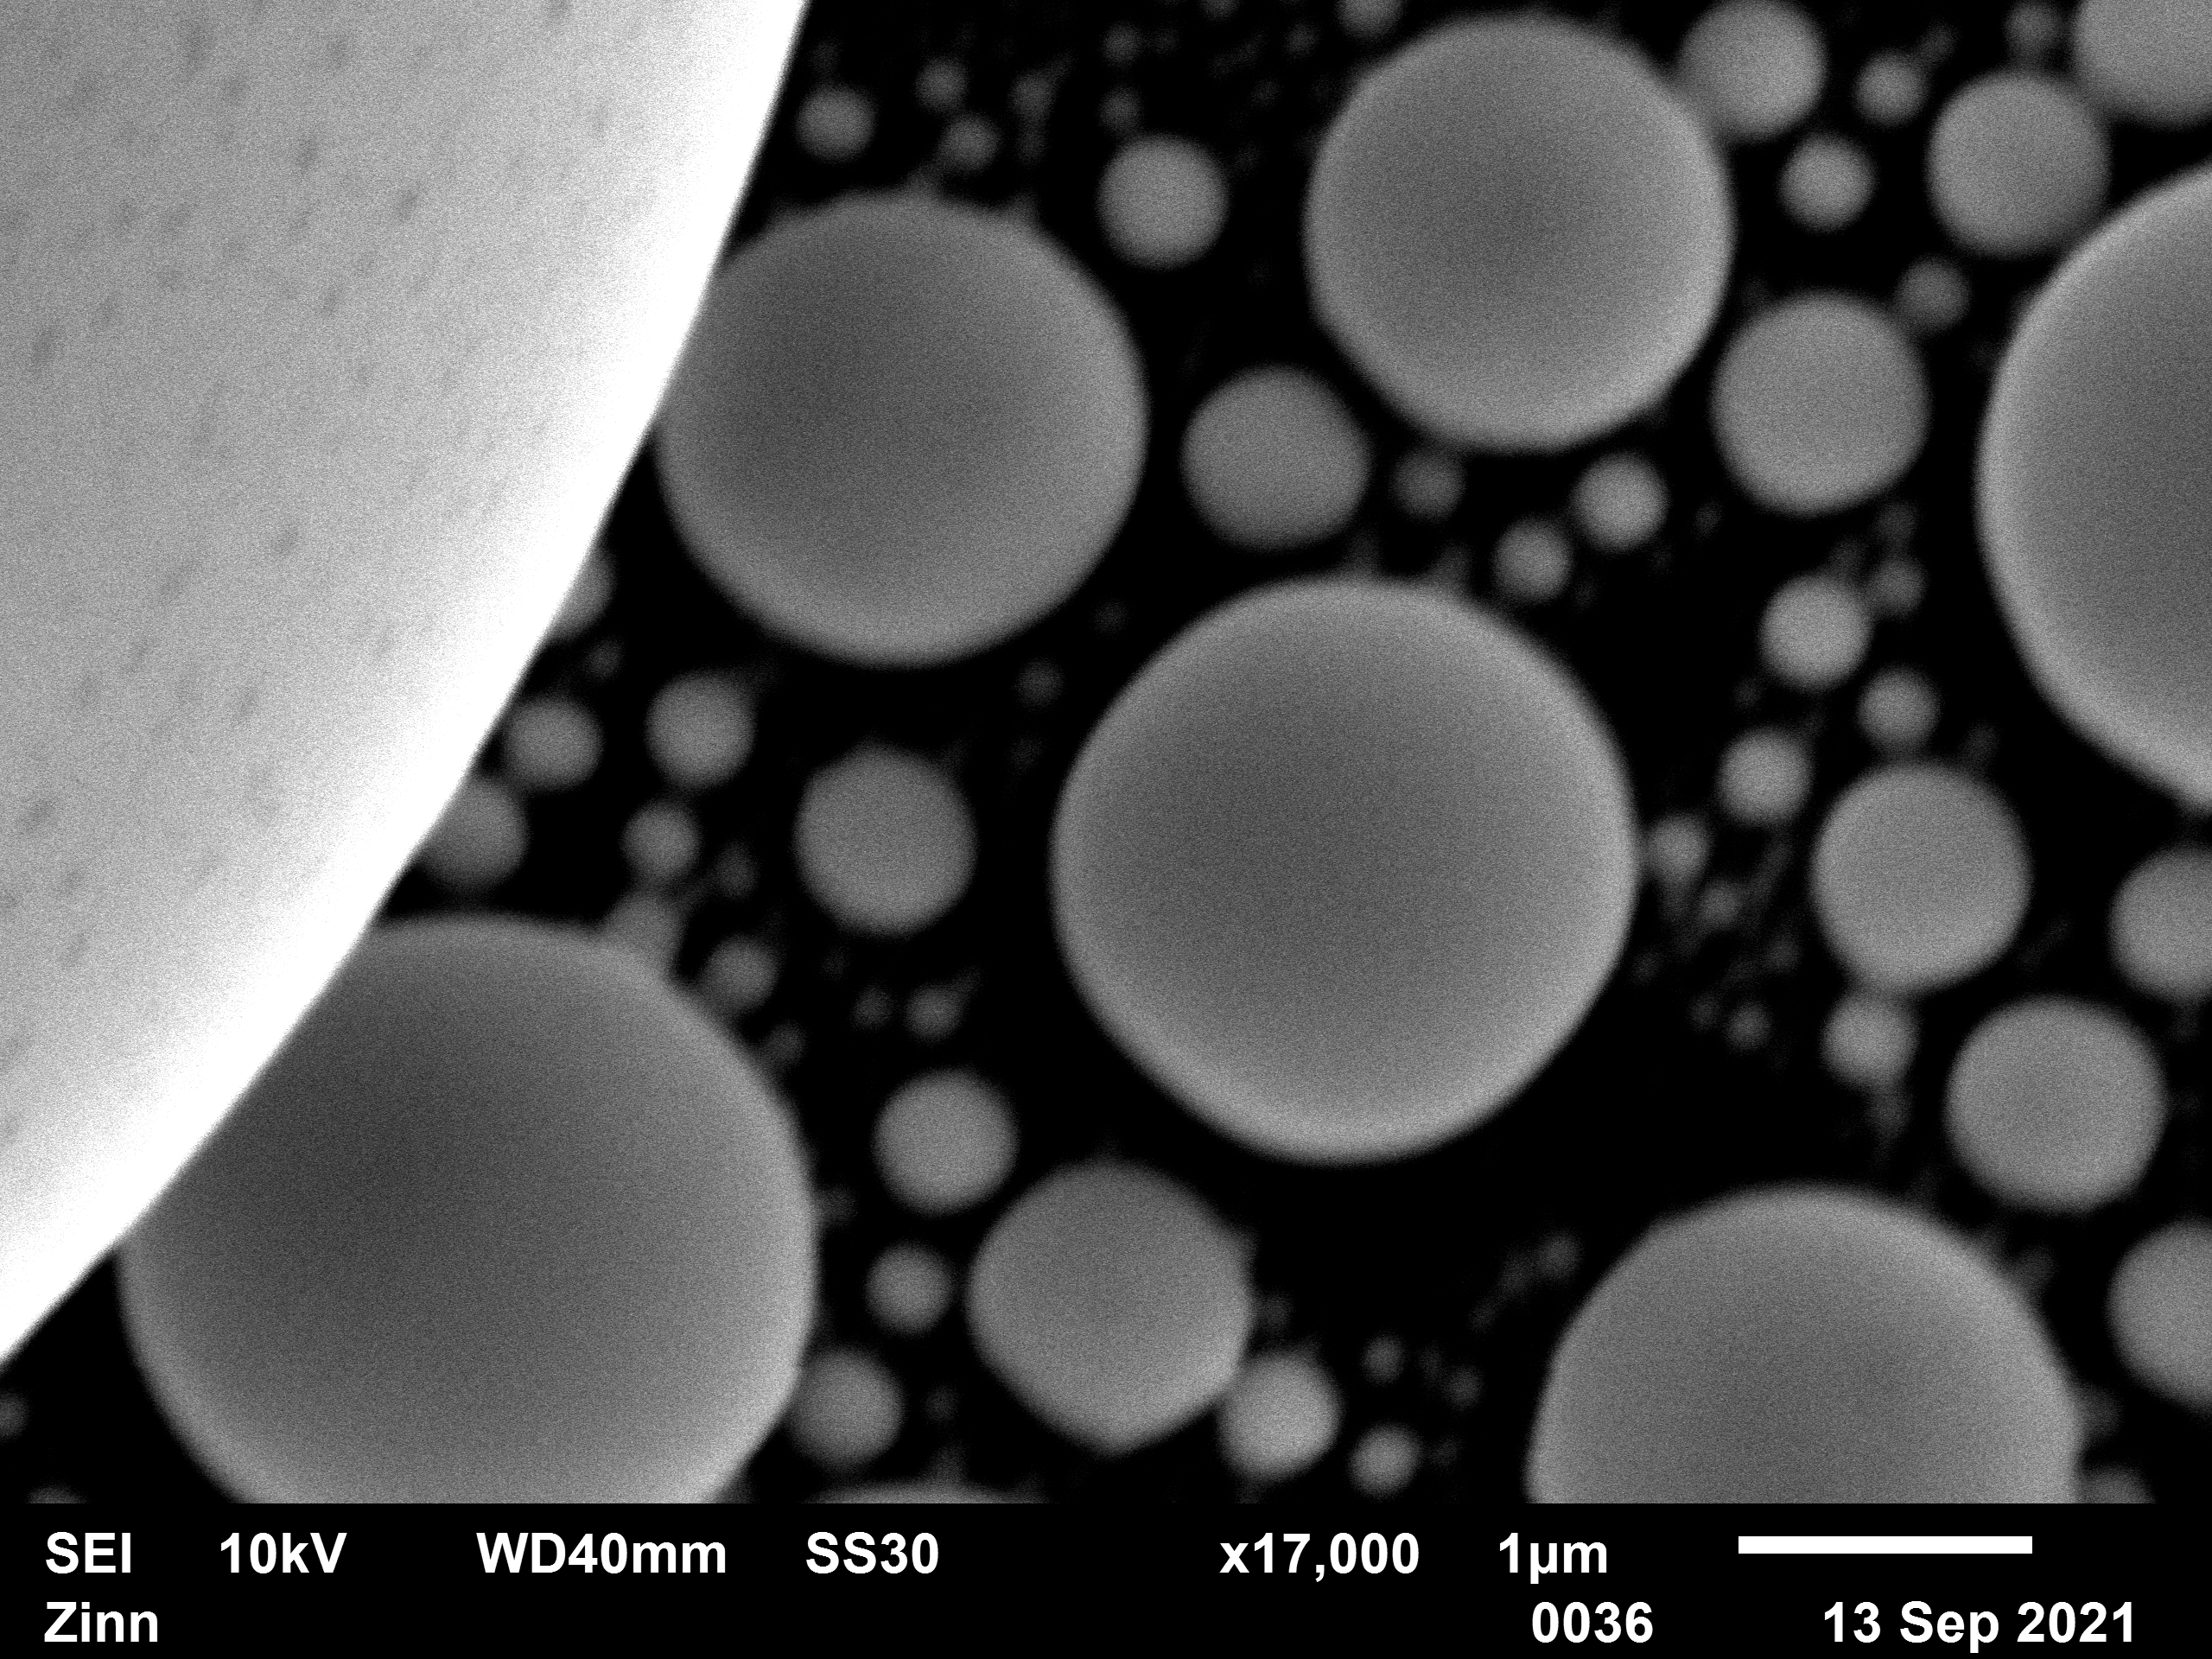
\includegraphics[width=\textwidth]{Auswertung/C/0036.png}
        \caption{10 kV}
    \end{subfigure}
    \hfill
    \begin{subfigure}[b]{0.45\textwidth}
        \centering
        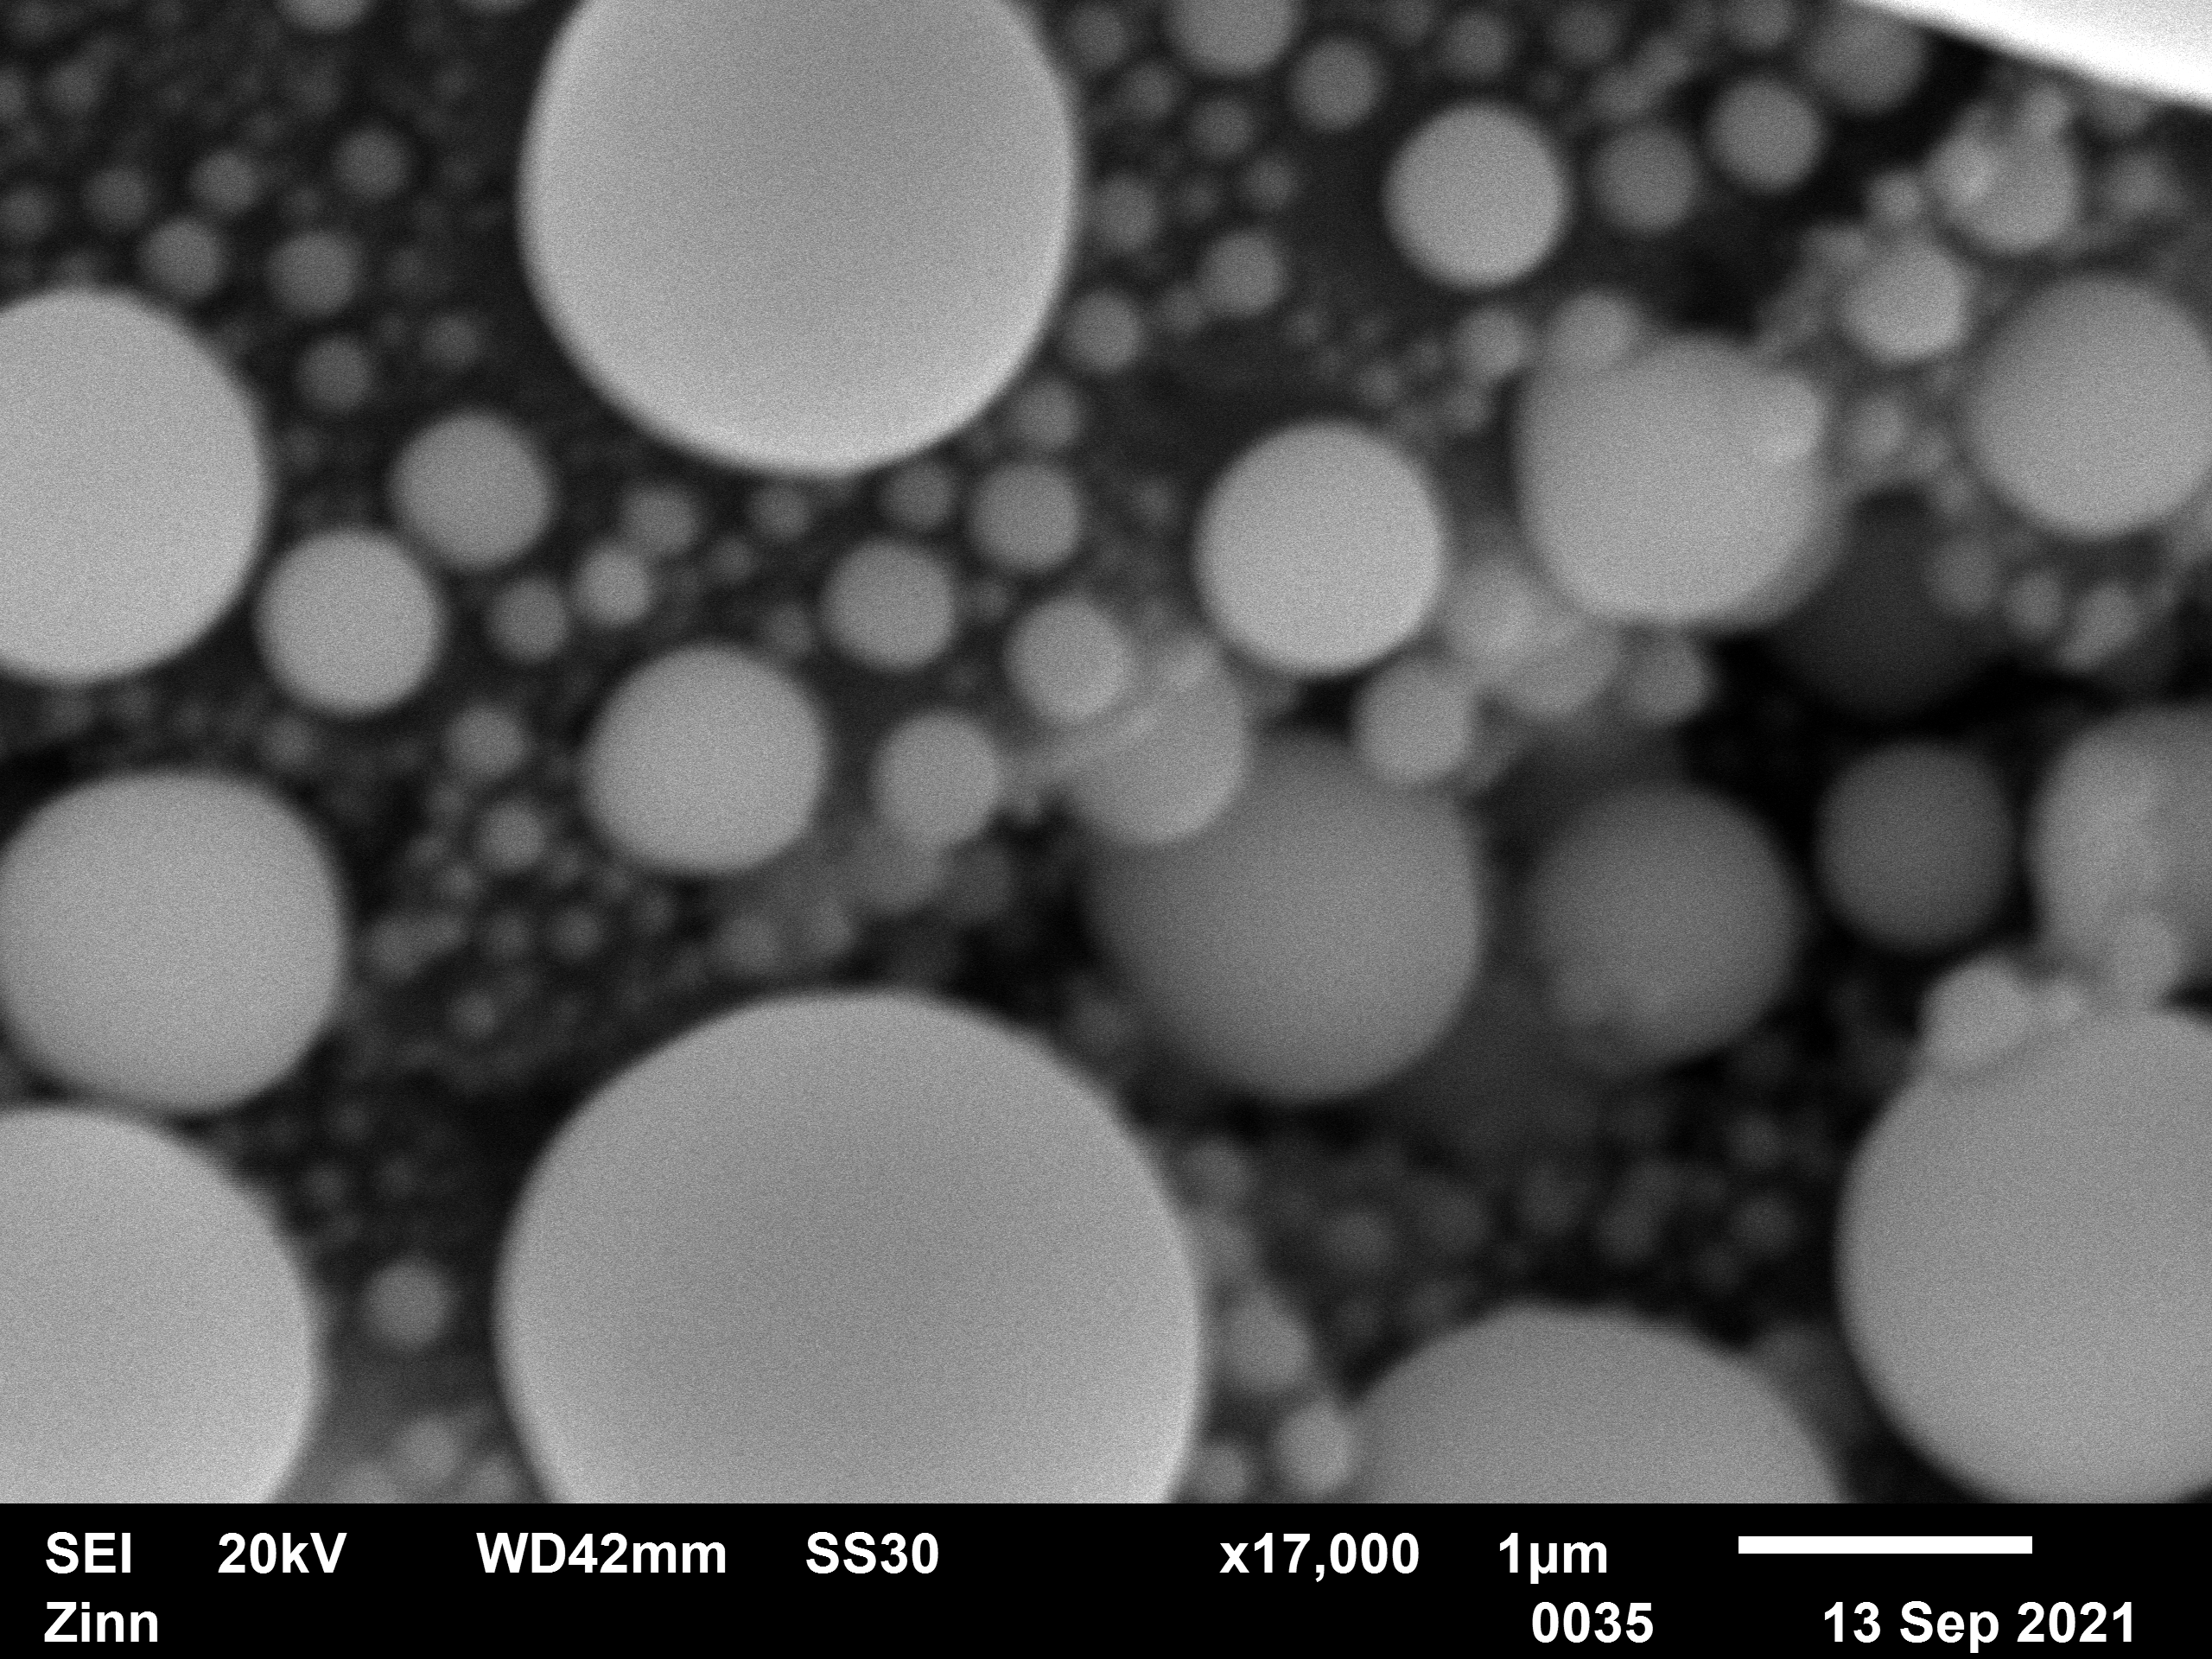
\includegraphics[width=\textwidth]{Auswertung/C/0035.png}
        \caption{20 kV}
    \end{subfigure}
    \\
    \begin{subfigure}[b]{0.45\textwidth}
        \centering
        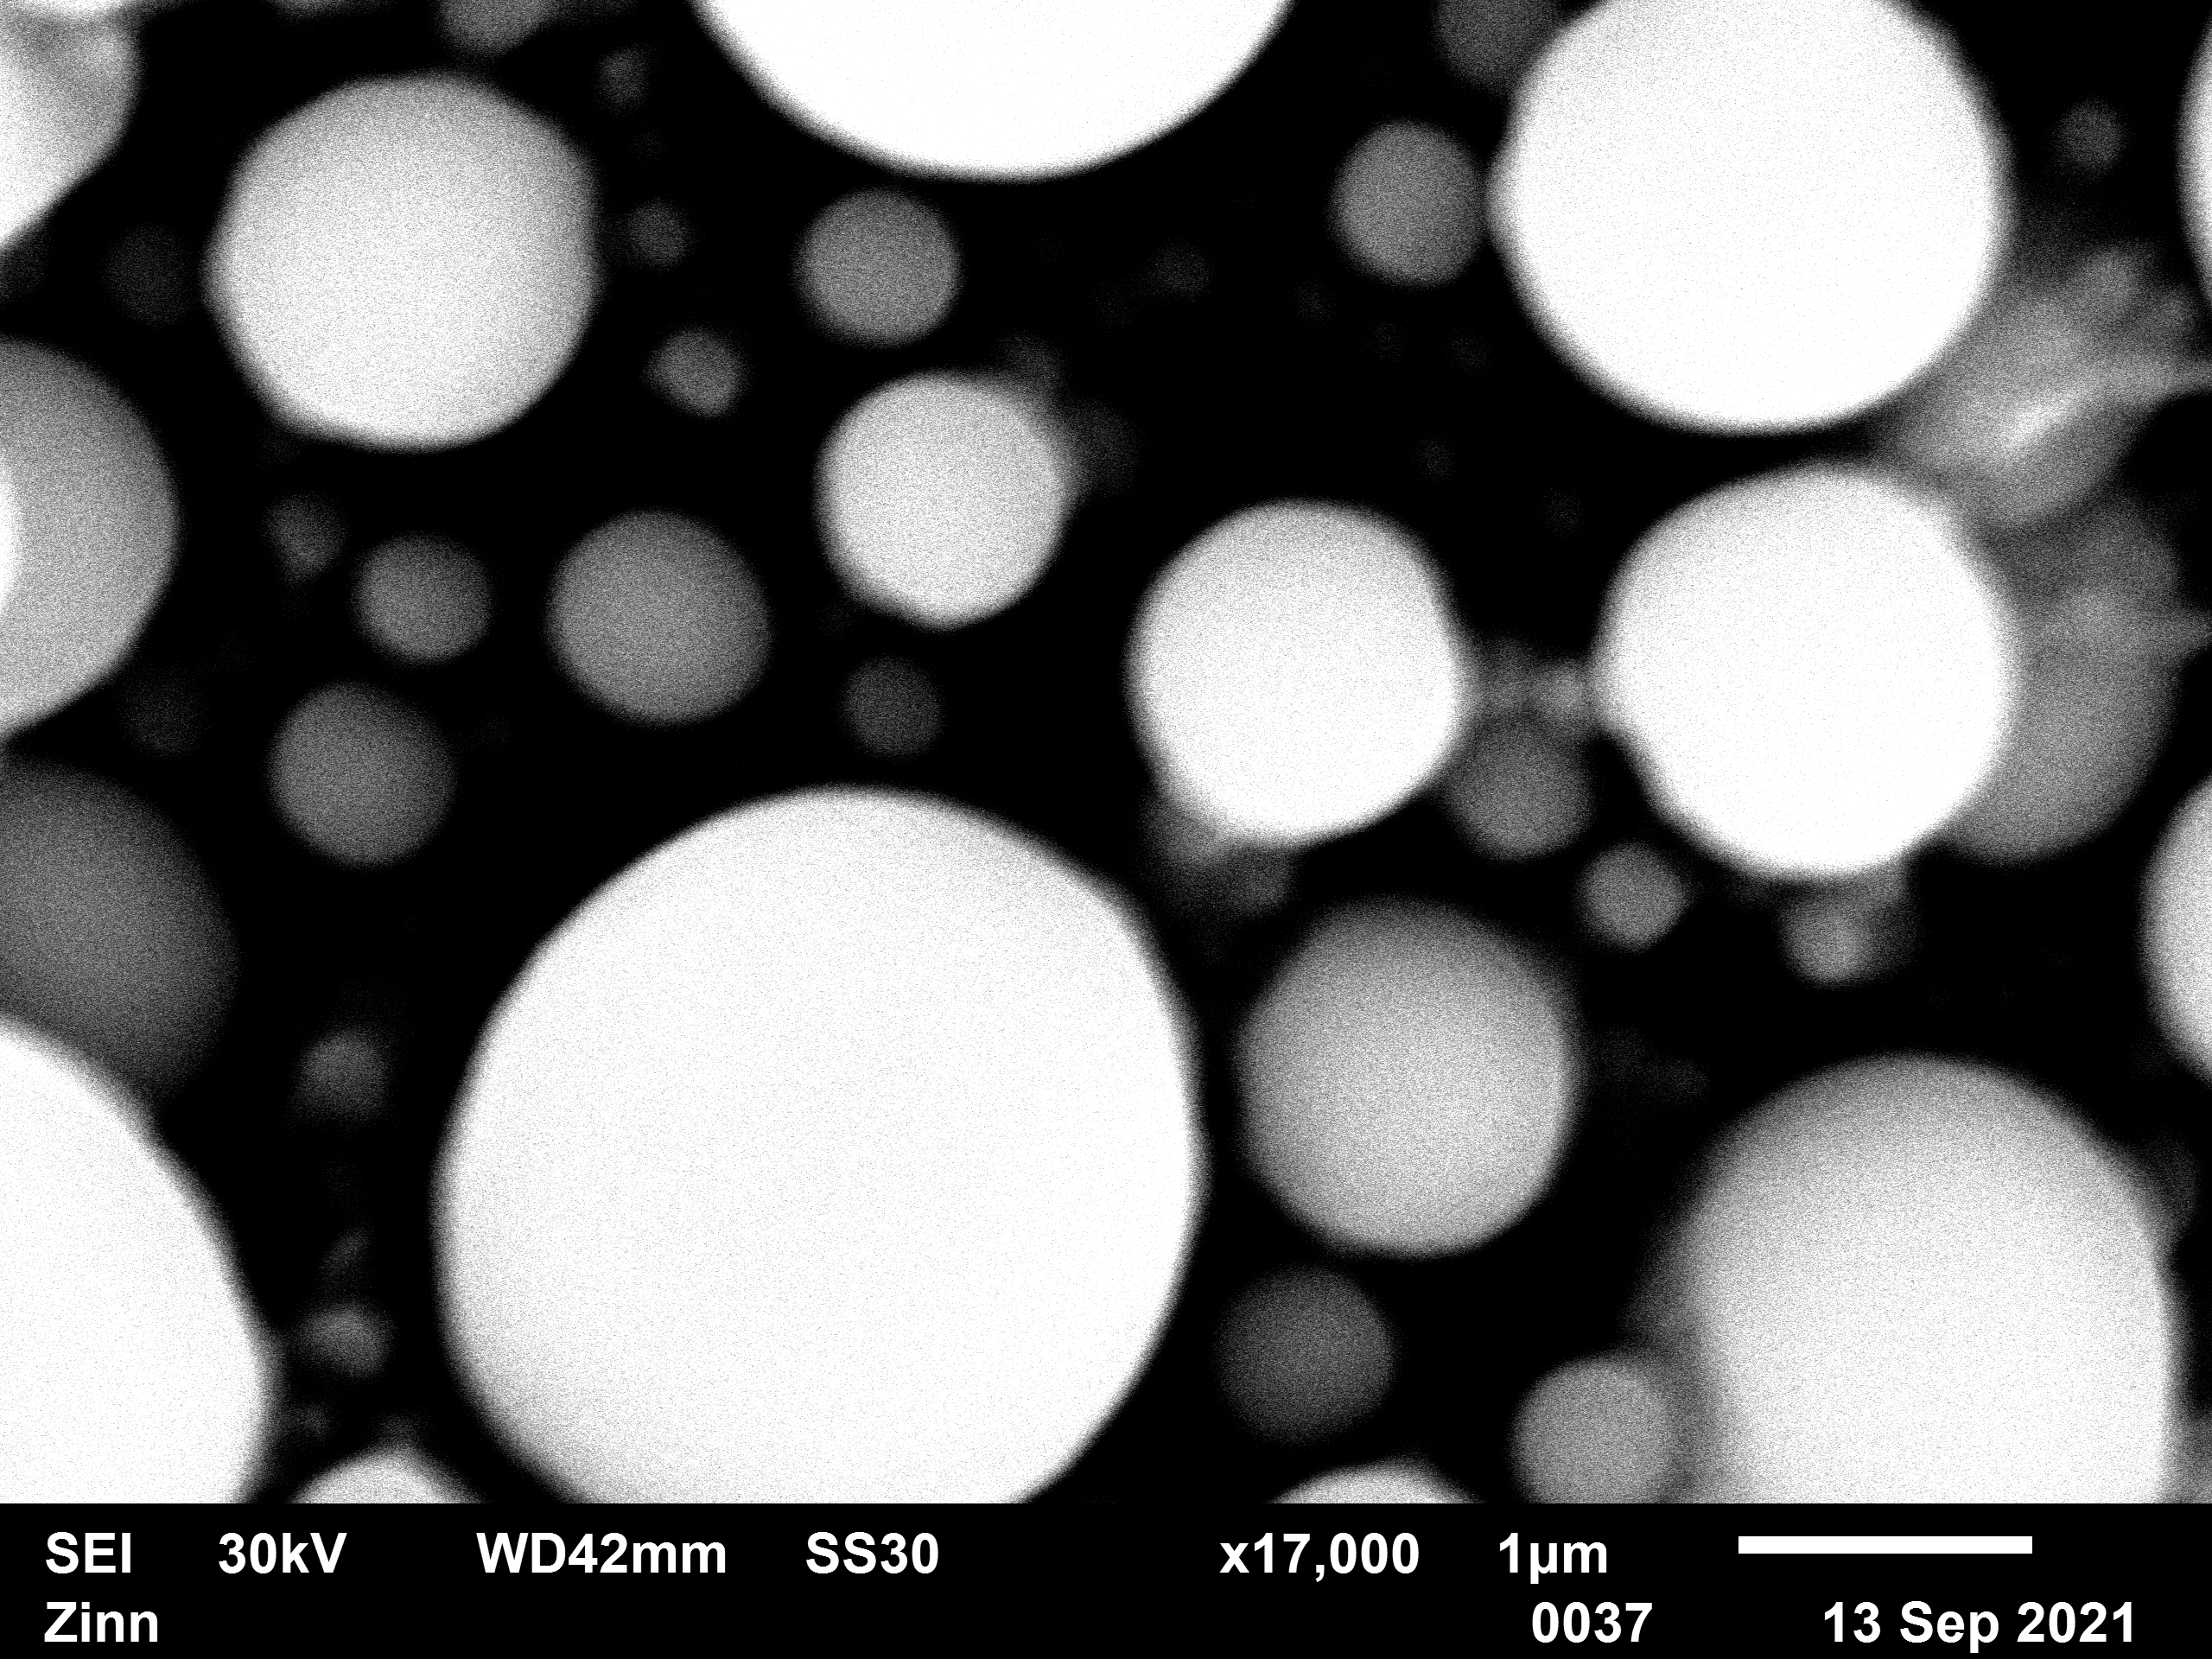
\includegraphics[width=\textwidth]{Auswertung/C/0037.png}
        \caption{30 kV}
    \end{subfigure}
    \caption{Zinstandart bei verschiedenen Beschleunigunsspannungen}
\end{figure}

Es fällt auf, dass bei 20 kV sehr viele Kugeln im Hintergrund zu erkennen sind, wohingegen dies bei 30 kV fast gar nicht mehr der Fall ist. Es scheint nicht so als würde die Beschleunigungsspannung hier einen konkreten Unterschied bewirken, da keine klare Tendenz zu erkennen ist. Jedoch haben wir auch hier das Problem, dass die Bildausschnitte nicht gut übereinstimmen. Darum gestaltet sich der Vergleich auch dementsprechend schwierig.

\newpage
Zum Schluss wurde dann der Arbeitsabstand variiert.
\begin{figure}[h]
    \centering
    
    \begin{subfigure}[b]{0.45\textwidth}
        \centering
        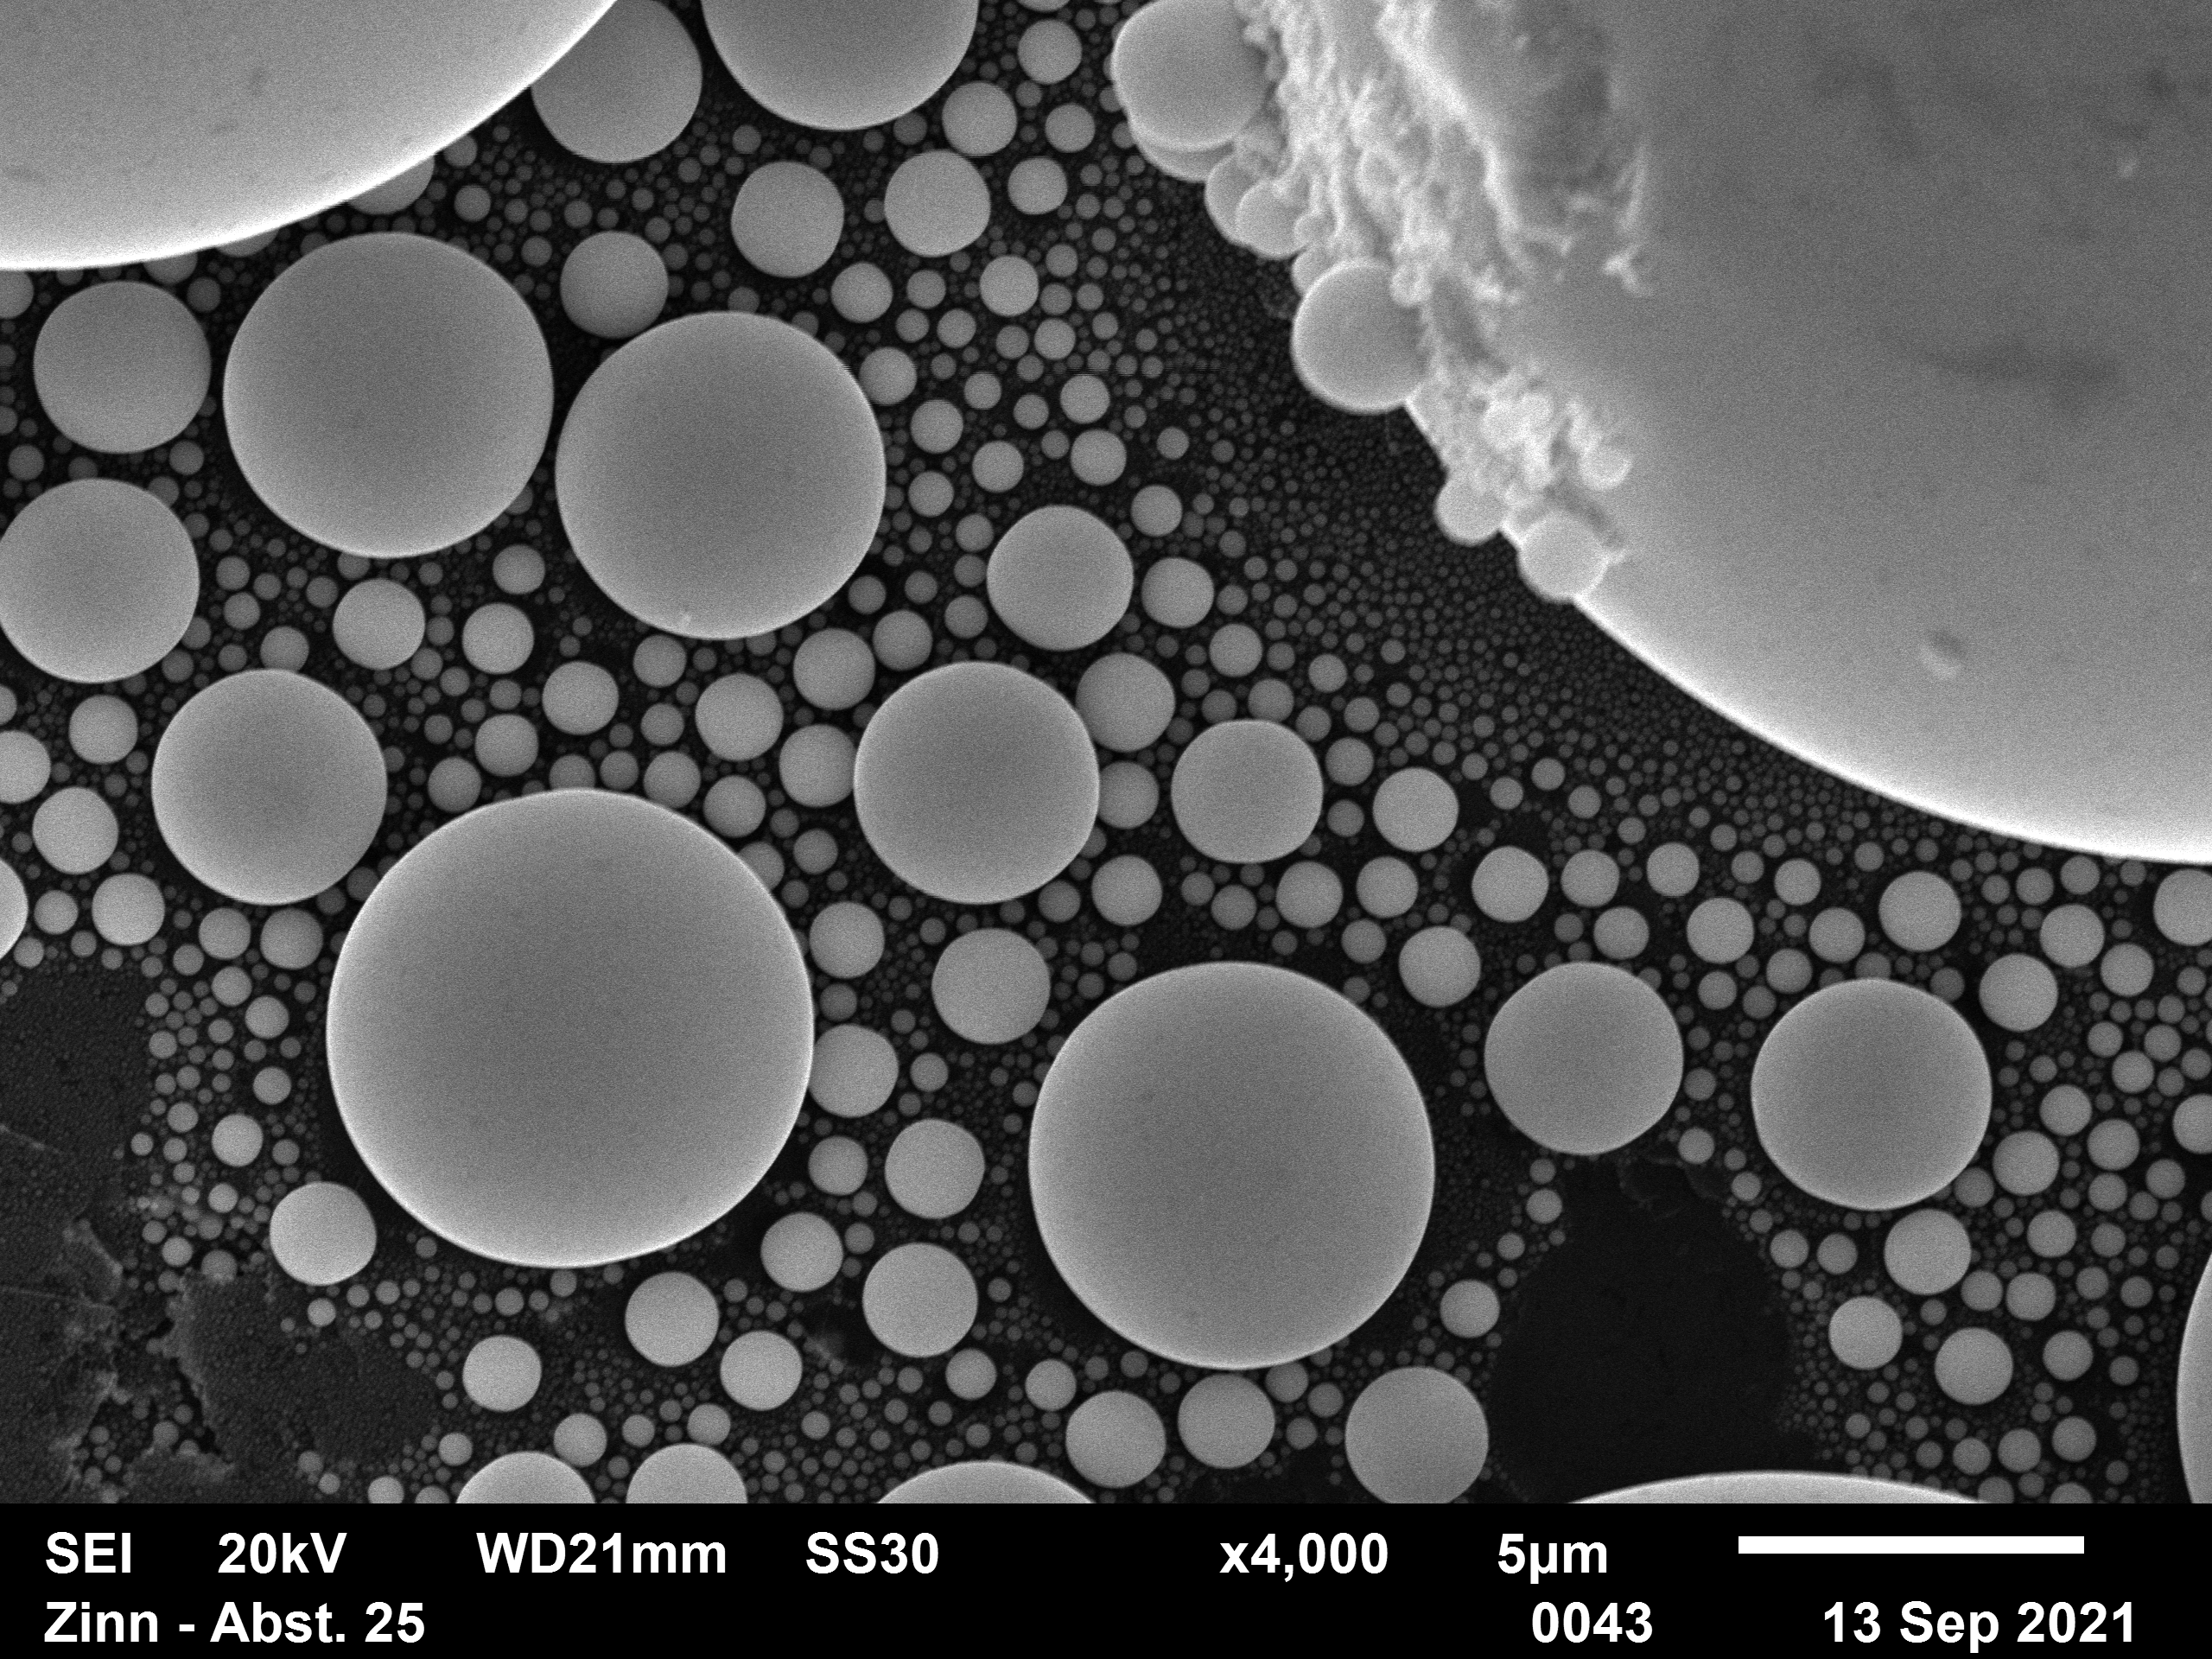
\includegraphics[width=\textwidth]{Auswertung/C/0043.png}
        \caption{Arbeitsabstand 25 mm}
    \end{subfigure}
    \hfill
    \begin{subfigure}[b]{0.45\textwidth}
        \centering
        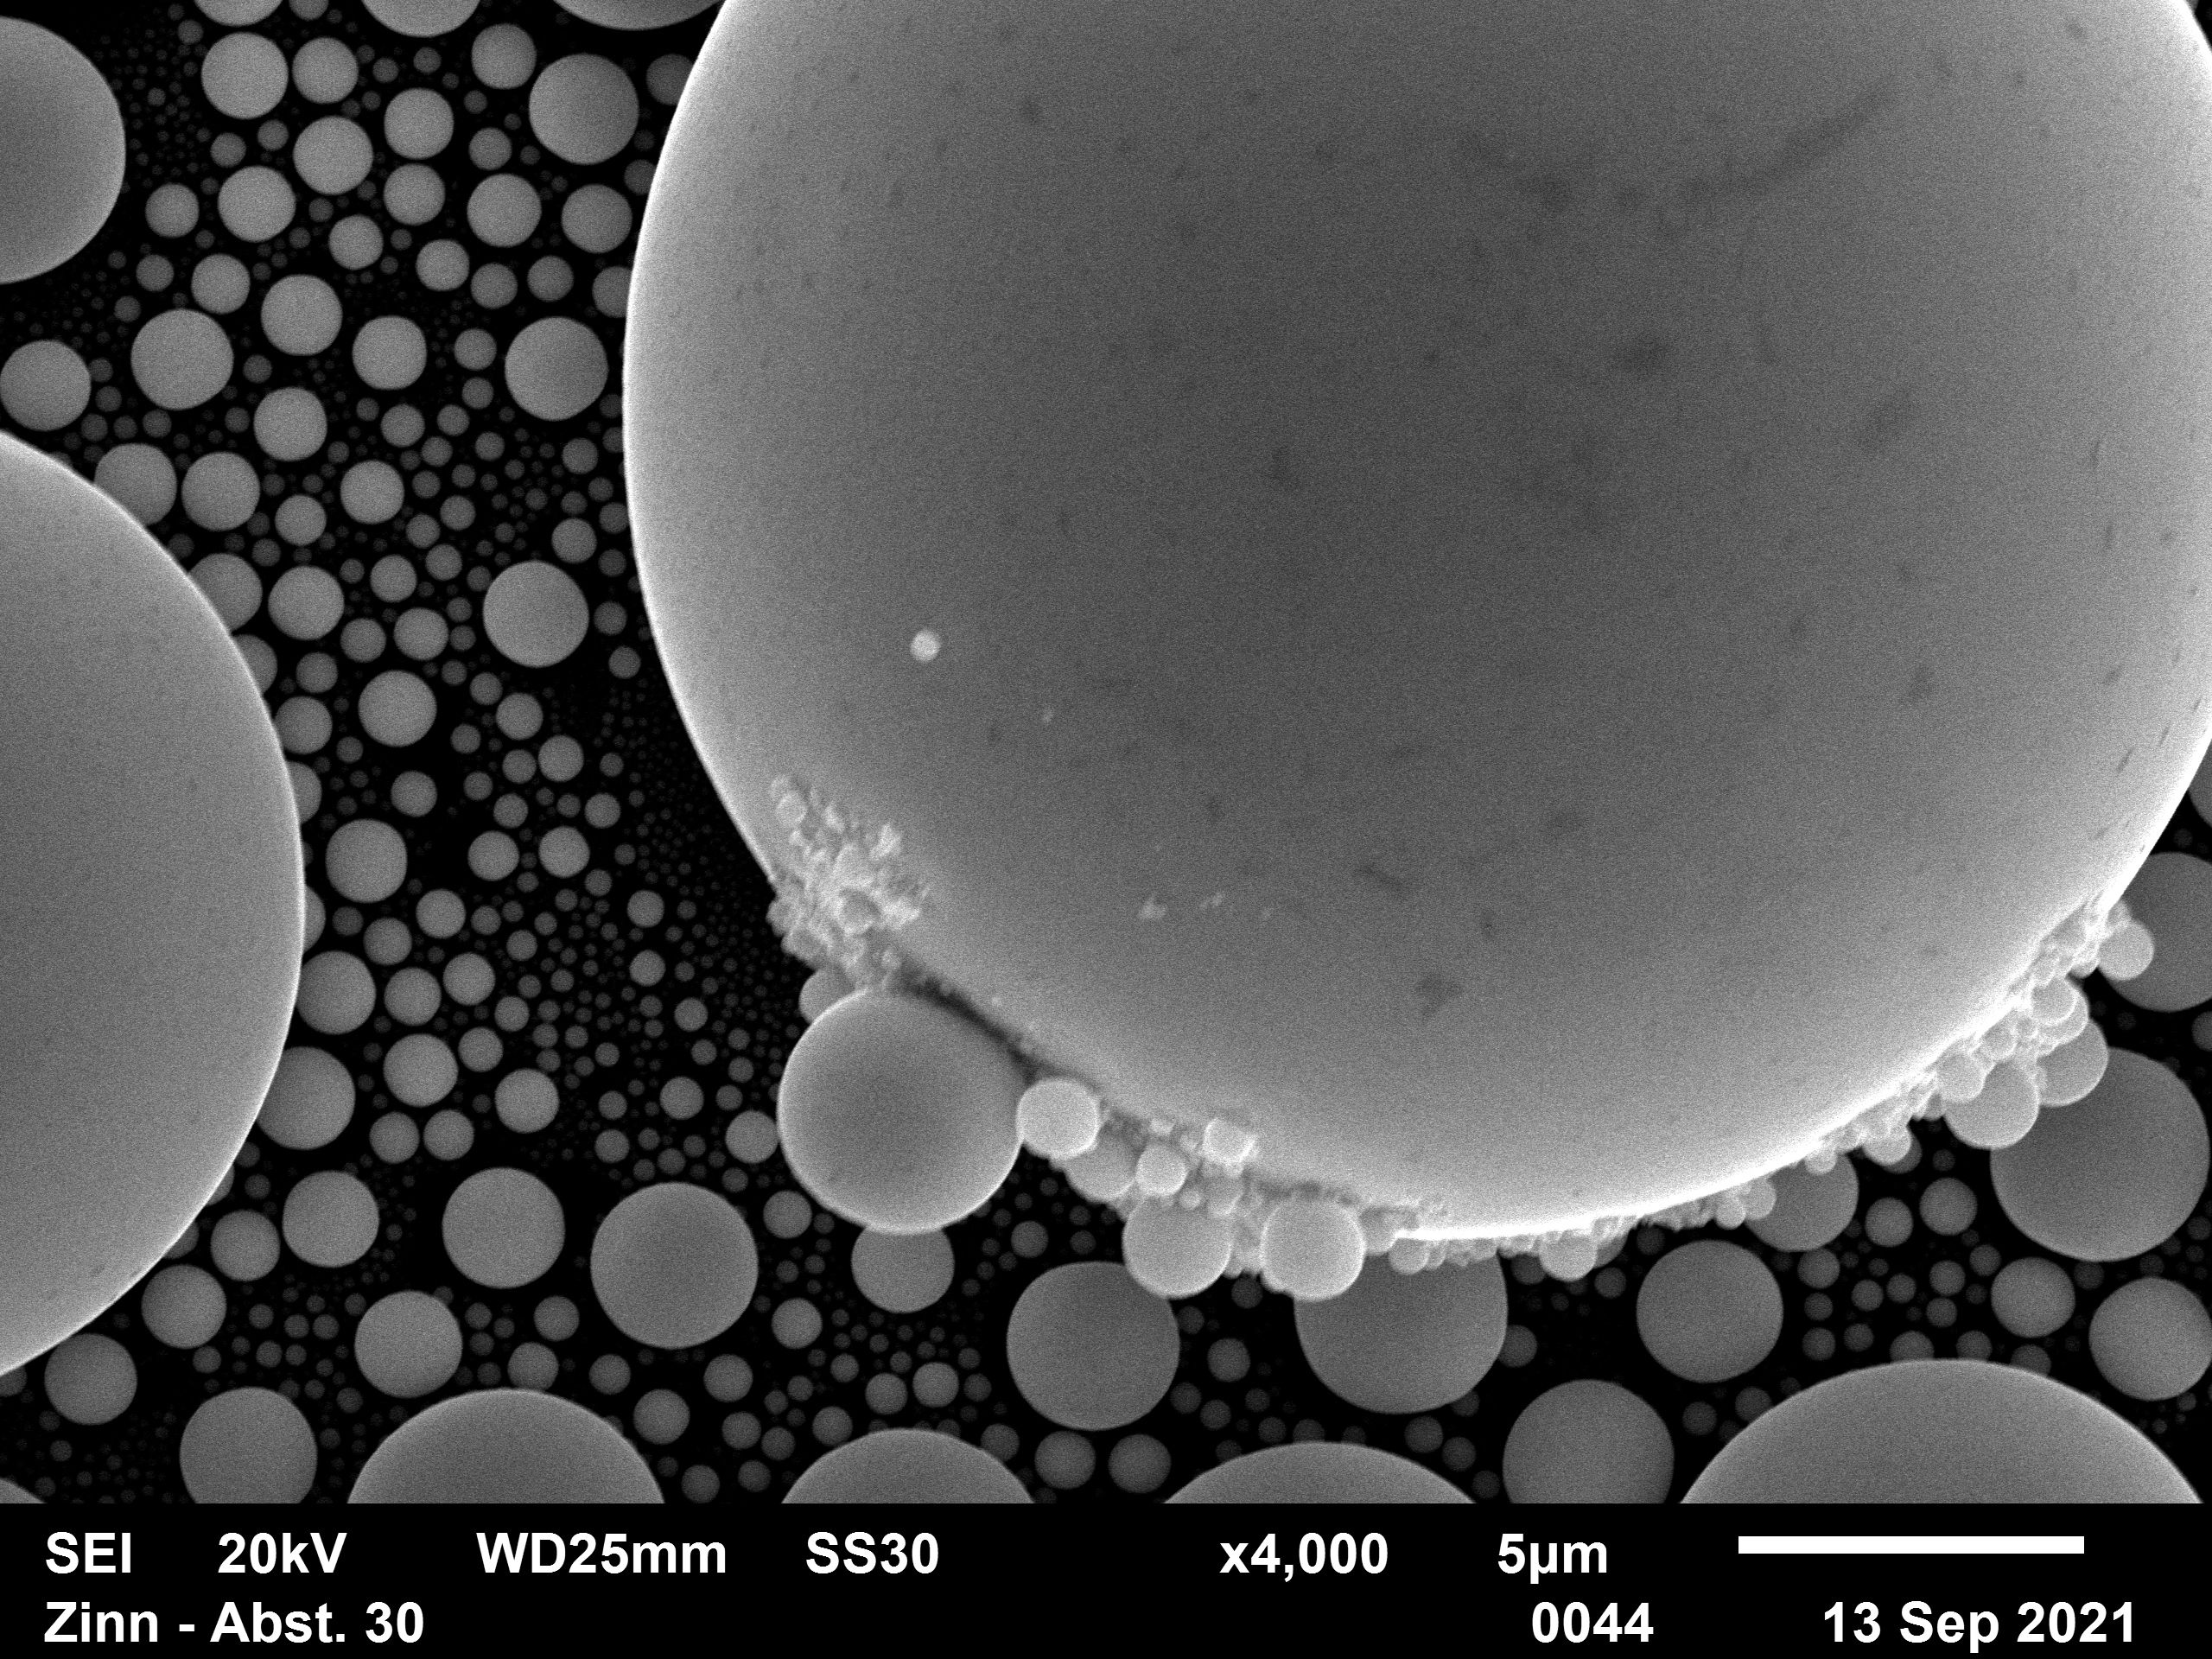
\includegraphics[width=\textwidth]{Auswertung/C/0044.png}
        \caption{Arbeitsabstand 30 mm}
    \end{subfigure}
    
    \caption{Zinnstandart bei unterschiedlichem Arbeitsabstand}
    \label{fig:43WD}
\end{figure}

Hier wurden bewusst nur zwei Bilder ausgewählt, da die Unterschied ausreichend deutlich zu erkennen sind. Außerdem dienen die kleinen Kugeln auf der Oberfläche der großen, in Abbildung \ref{fig:43WD} als Landmarken.
In Bezug auf den Arbeitsabstand fällt auf, dass mit dessen Verringerung mehrere kleinere Kugeln in den hinteren Ebenen zu erkennen sind.

\newpage
\section{Gebrochene Schraube}

In folgenden Versuchsteil soll die Bruchuhrsache einer Schraube ermittelt werden.

Im ersten Schritt wurden hierzu Bilder der Bruchfläche mit verschiedenen Detektoren aufgenommen.
\begin{figure}[h]
    \centering
    
    \begin{subfigure}[b]{0.45\textwidth}
        \centering
        \includegraphics[width=\textwidth]{Auswertung/D/0049.png}
        \caption{SEI}
    \end{subfigure}
    \hfill
    \begin{subfigure}[b]{0.45\textwidth}
        \centering
        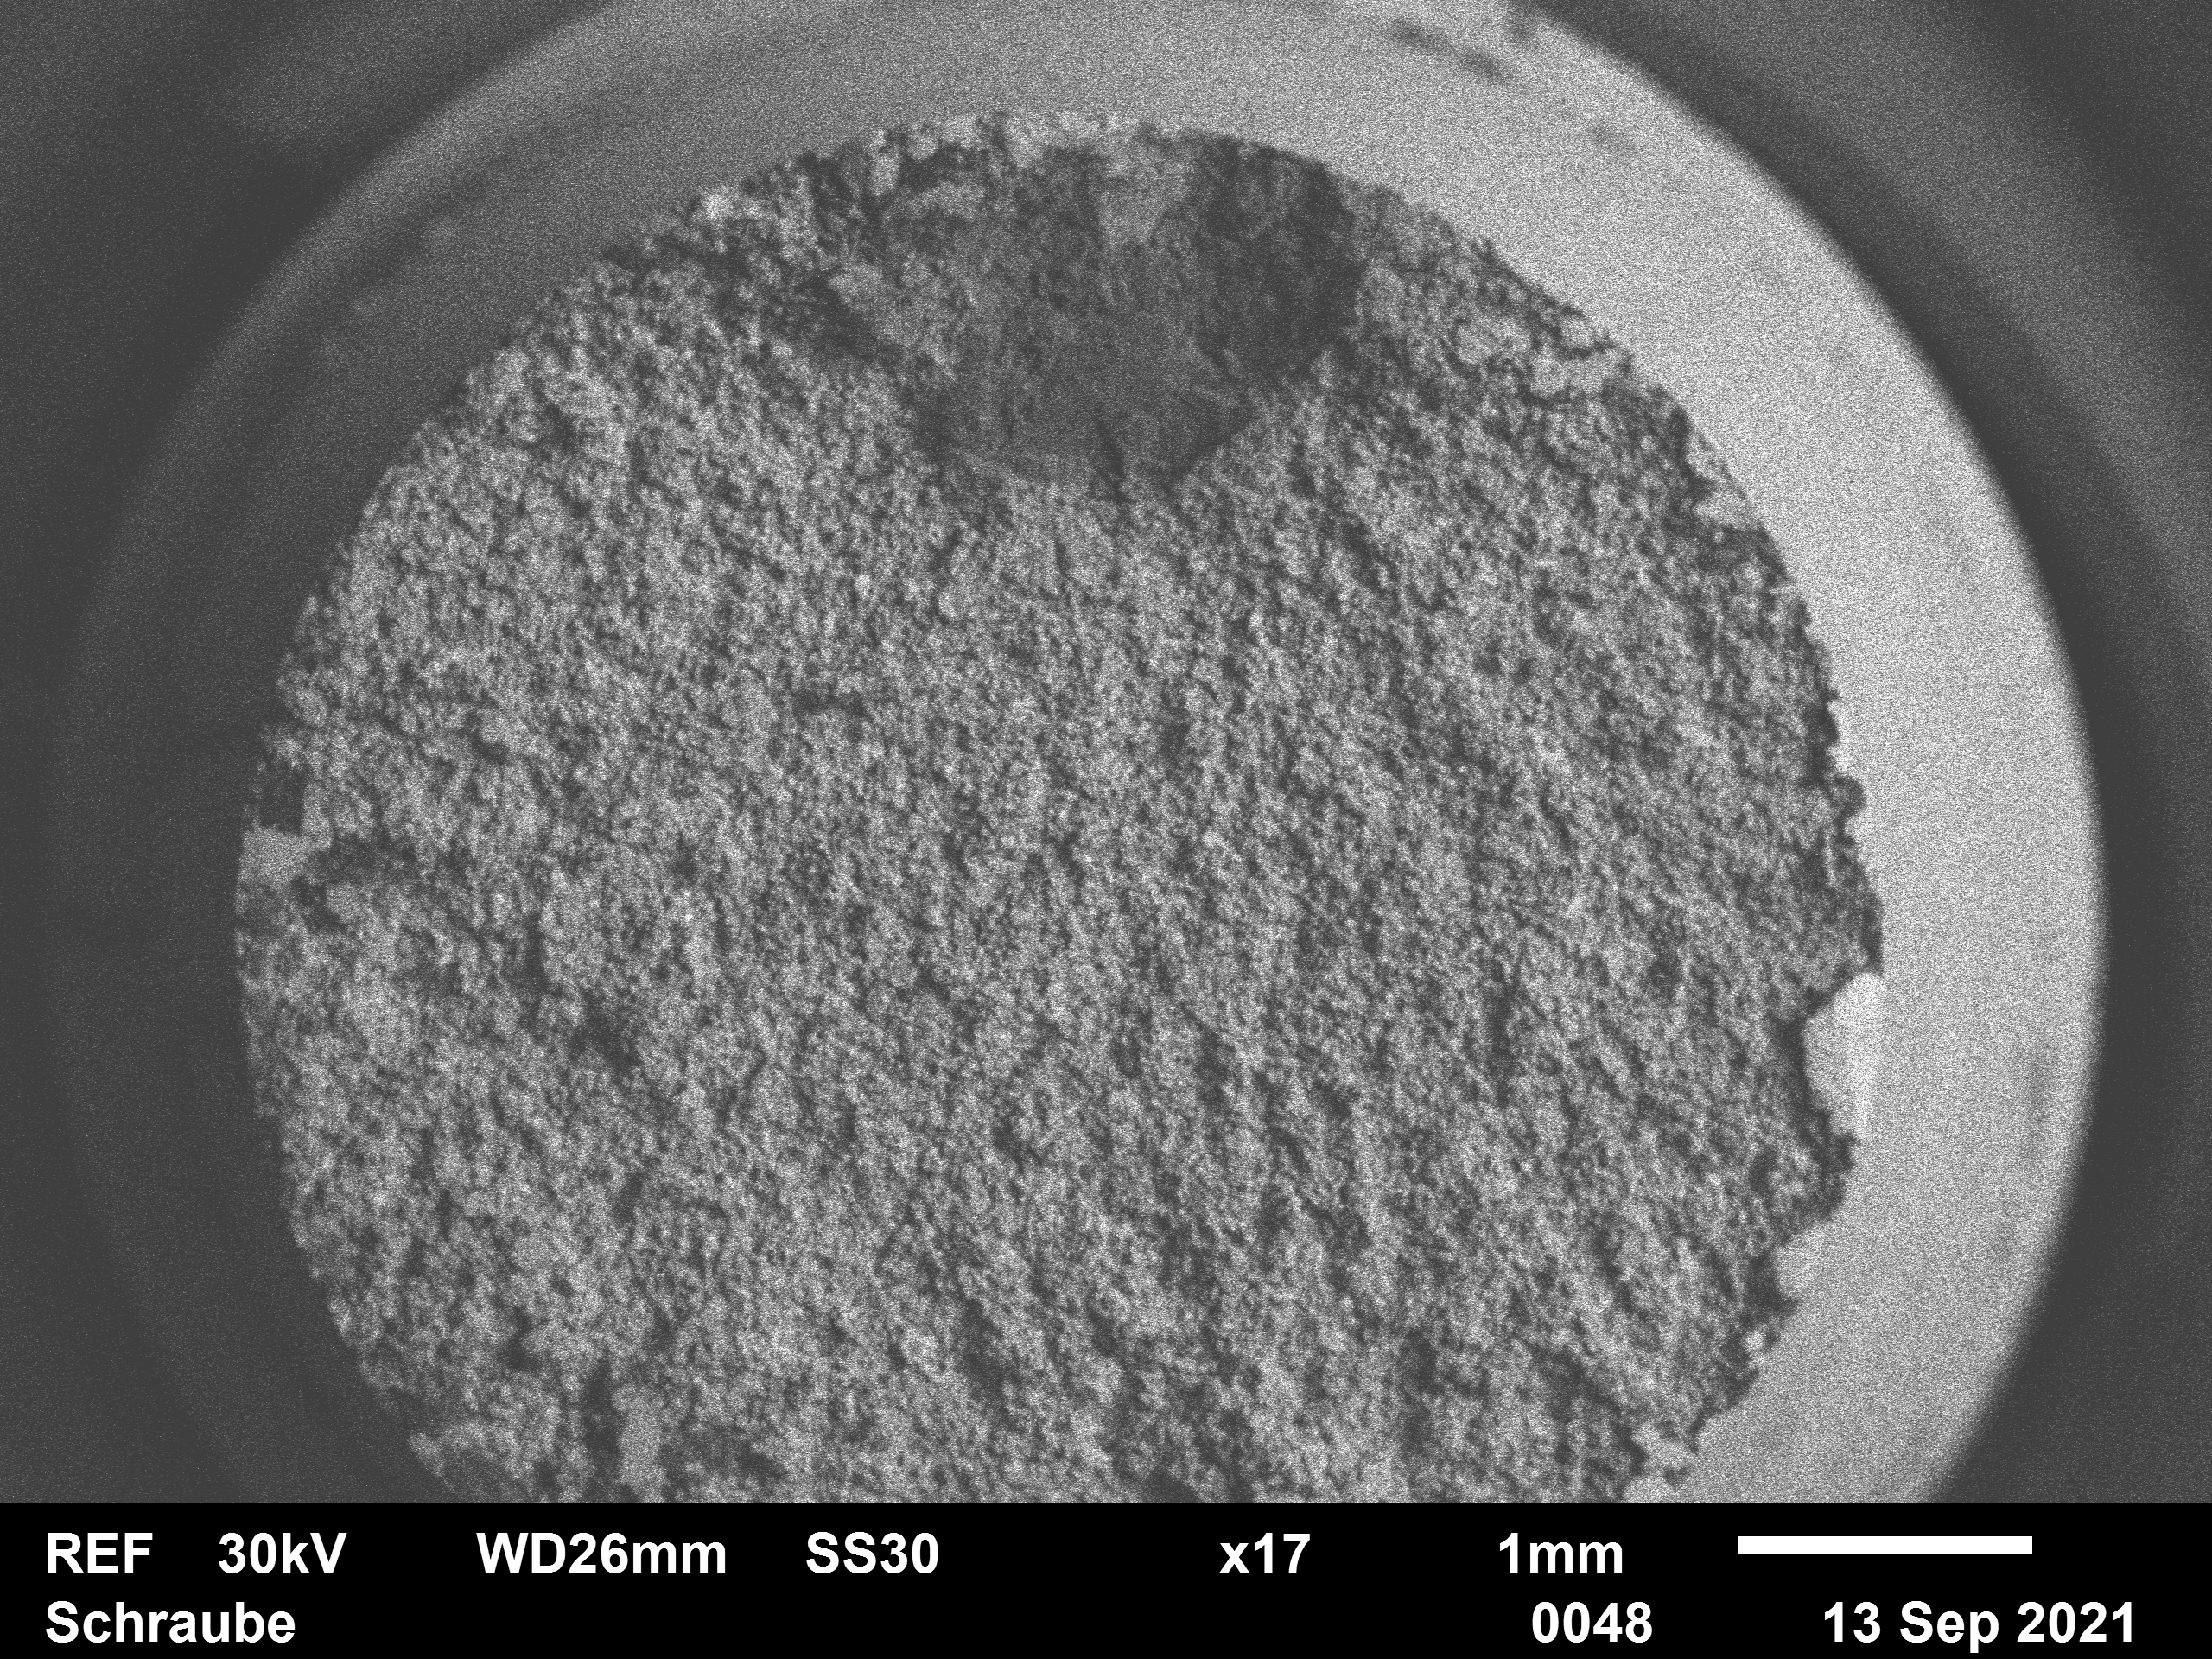
\includegraphics[width=\textwidth]{Auswertung/D/0048.png}
        \caption{REF}
    \end{subfigure}
    \\
    \begin{subfigure}[b]{0.45\textwidth}
        \centering
        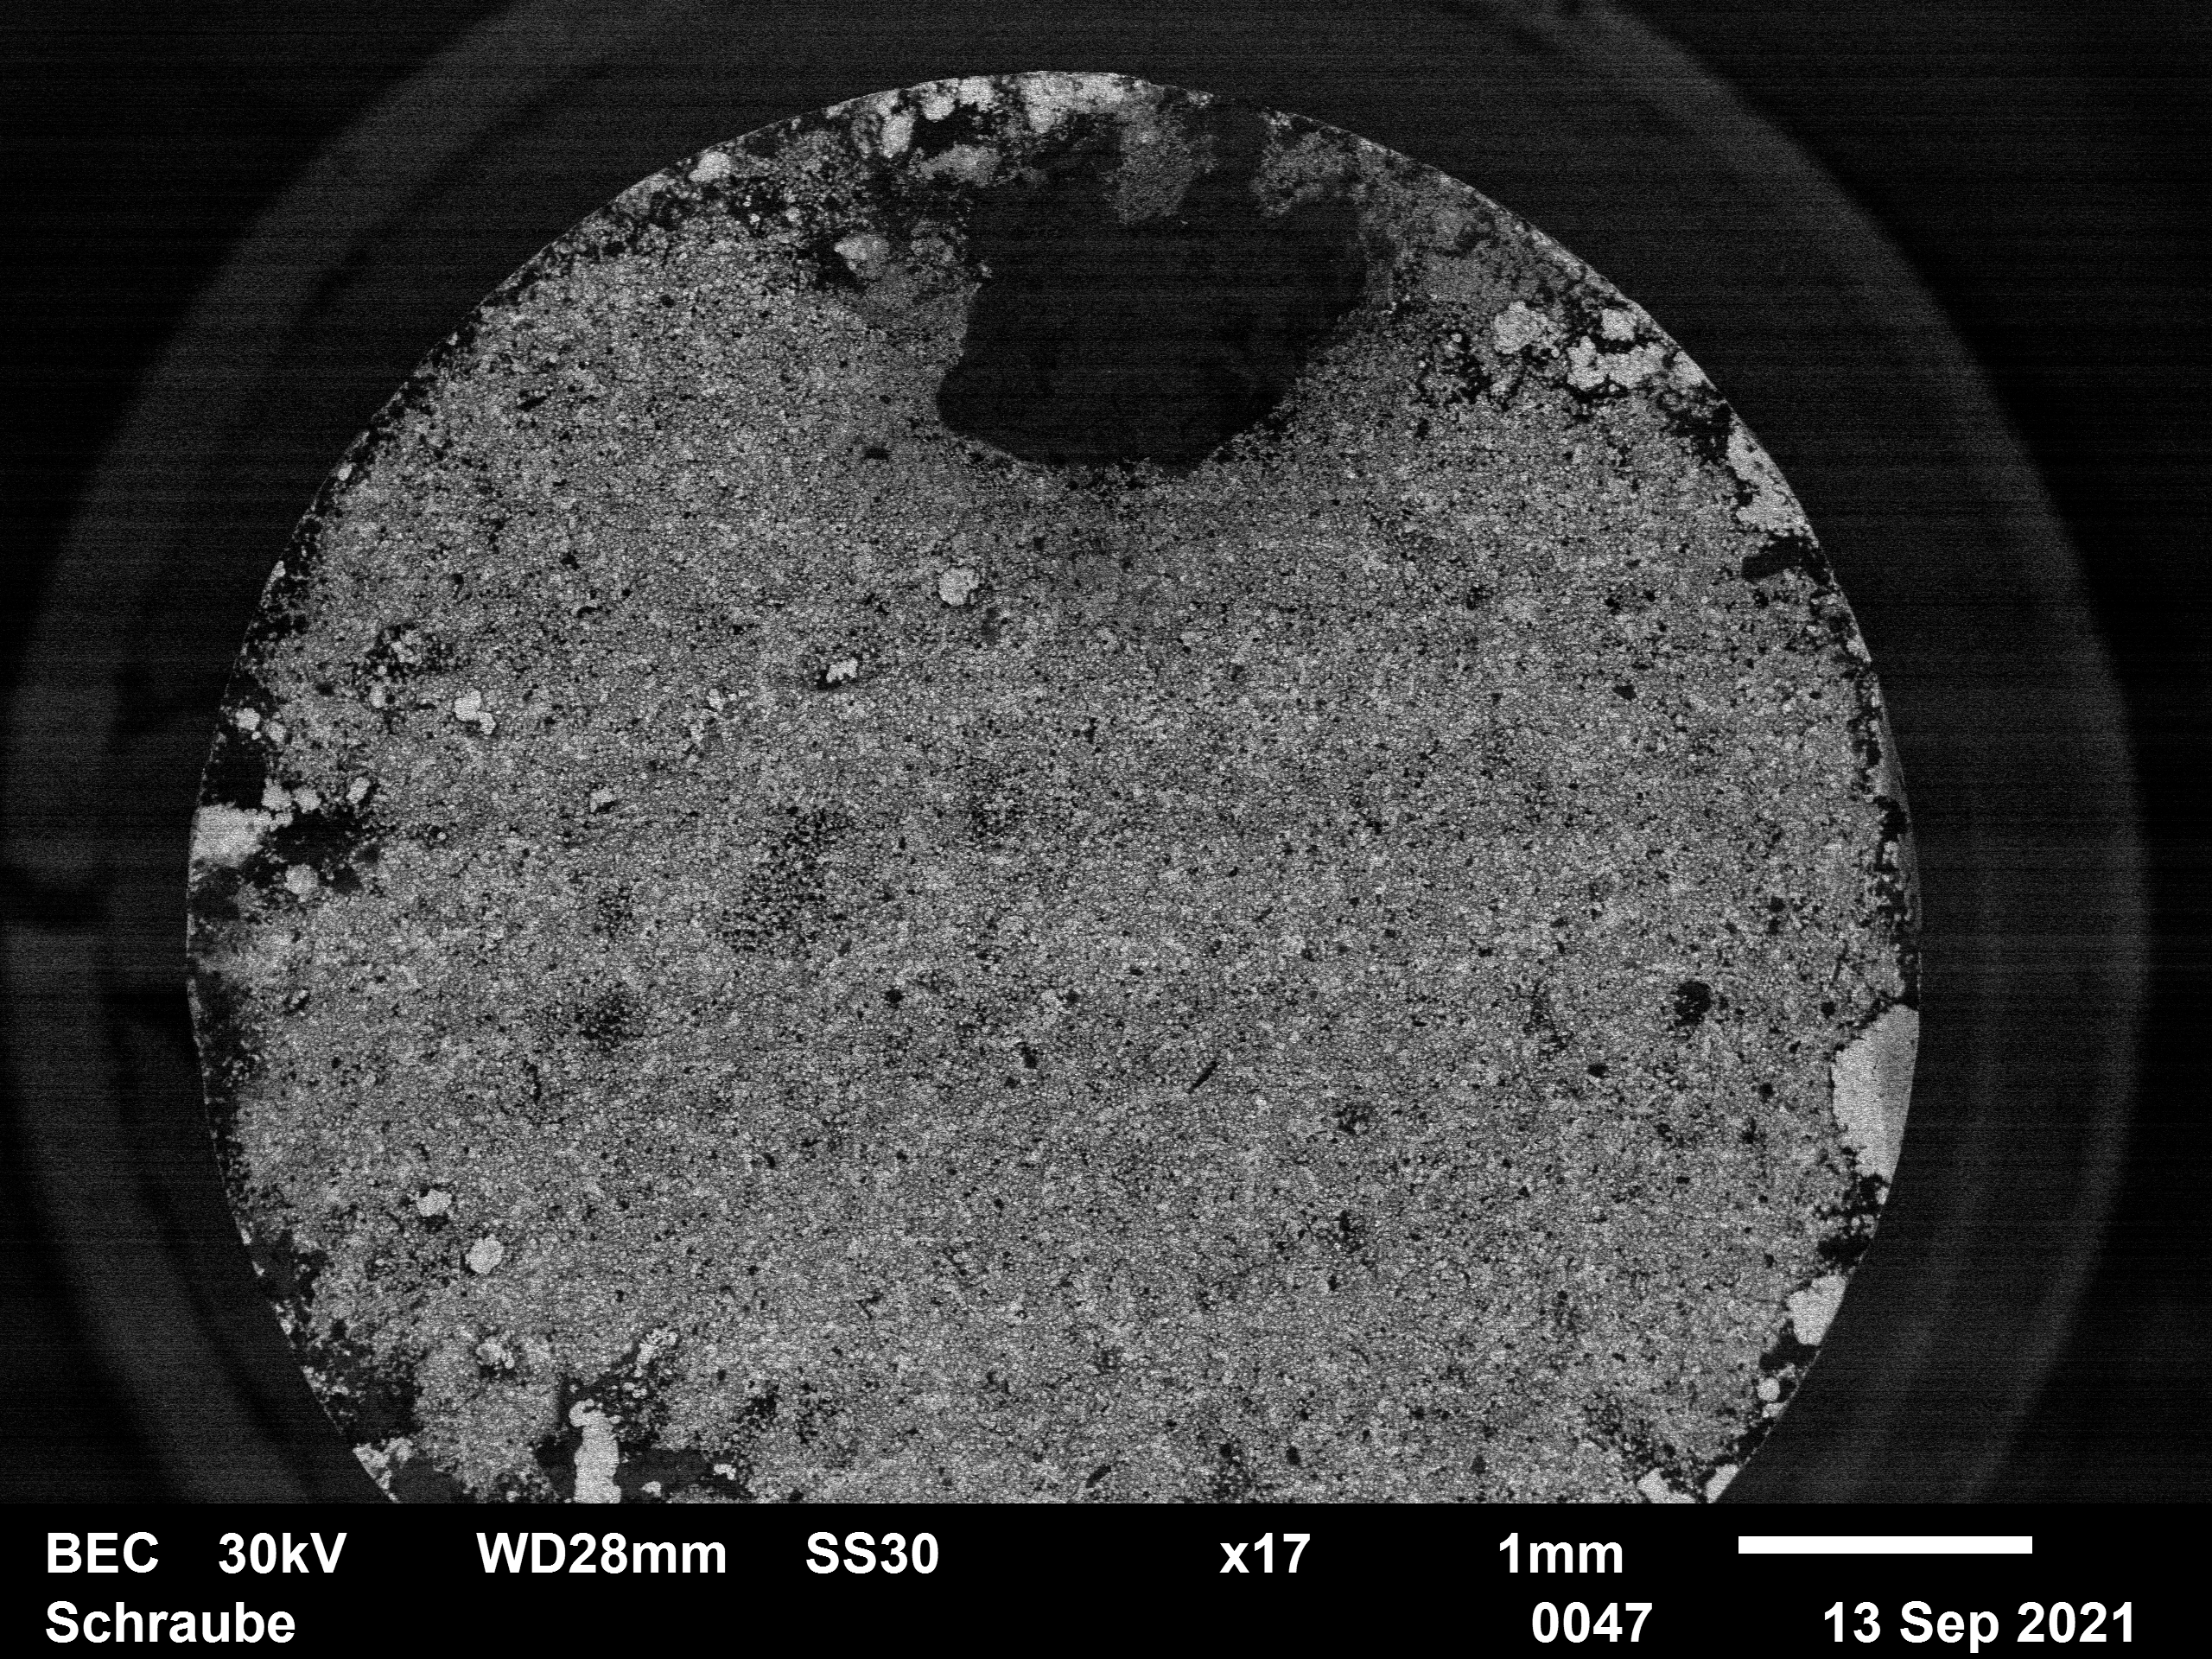
\includegraphics[width=\textwidth]{Auswertung/D/0047.png}
        \caption{BEC}
    \end{subfigure}
    \caption{Bruchfläche der Schraube mit unterschiedlichen Detektoren}
\end{figure}
Für einen ersten Eindruck wurde der SEI Modus verwendet, um die Struktur der Fläche zu untersuchen, wurde der REF Modus verwendet. In allen Aufnahmen und besonders im letzten Bild, im BEC Modus, sind drei unterschiedliche Zonen, bzgl. der Helligkeit, zu erkennen. Zum Einen ein recht auffälliger dunkler Fleck im oberen Teil, daneben mehrere kleine hellere Zonen, die sich am Rand der Fläche zu konzentrieren und der übrige Teil der Schraube, dessen Helligkeit zwischen den beiden anderen Zonen liegt. \\

\newpage
Als Nächstes wurde eine Nahaufnahme des dunklen Flecks angefertigt.
\begin{figure}[h]
    \centering
    
    \begin{subfigure}[b]{0.45\textwidth}
        \centering
        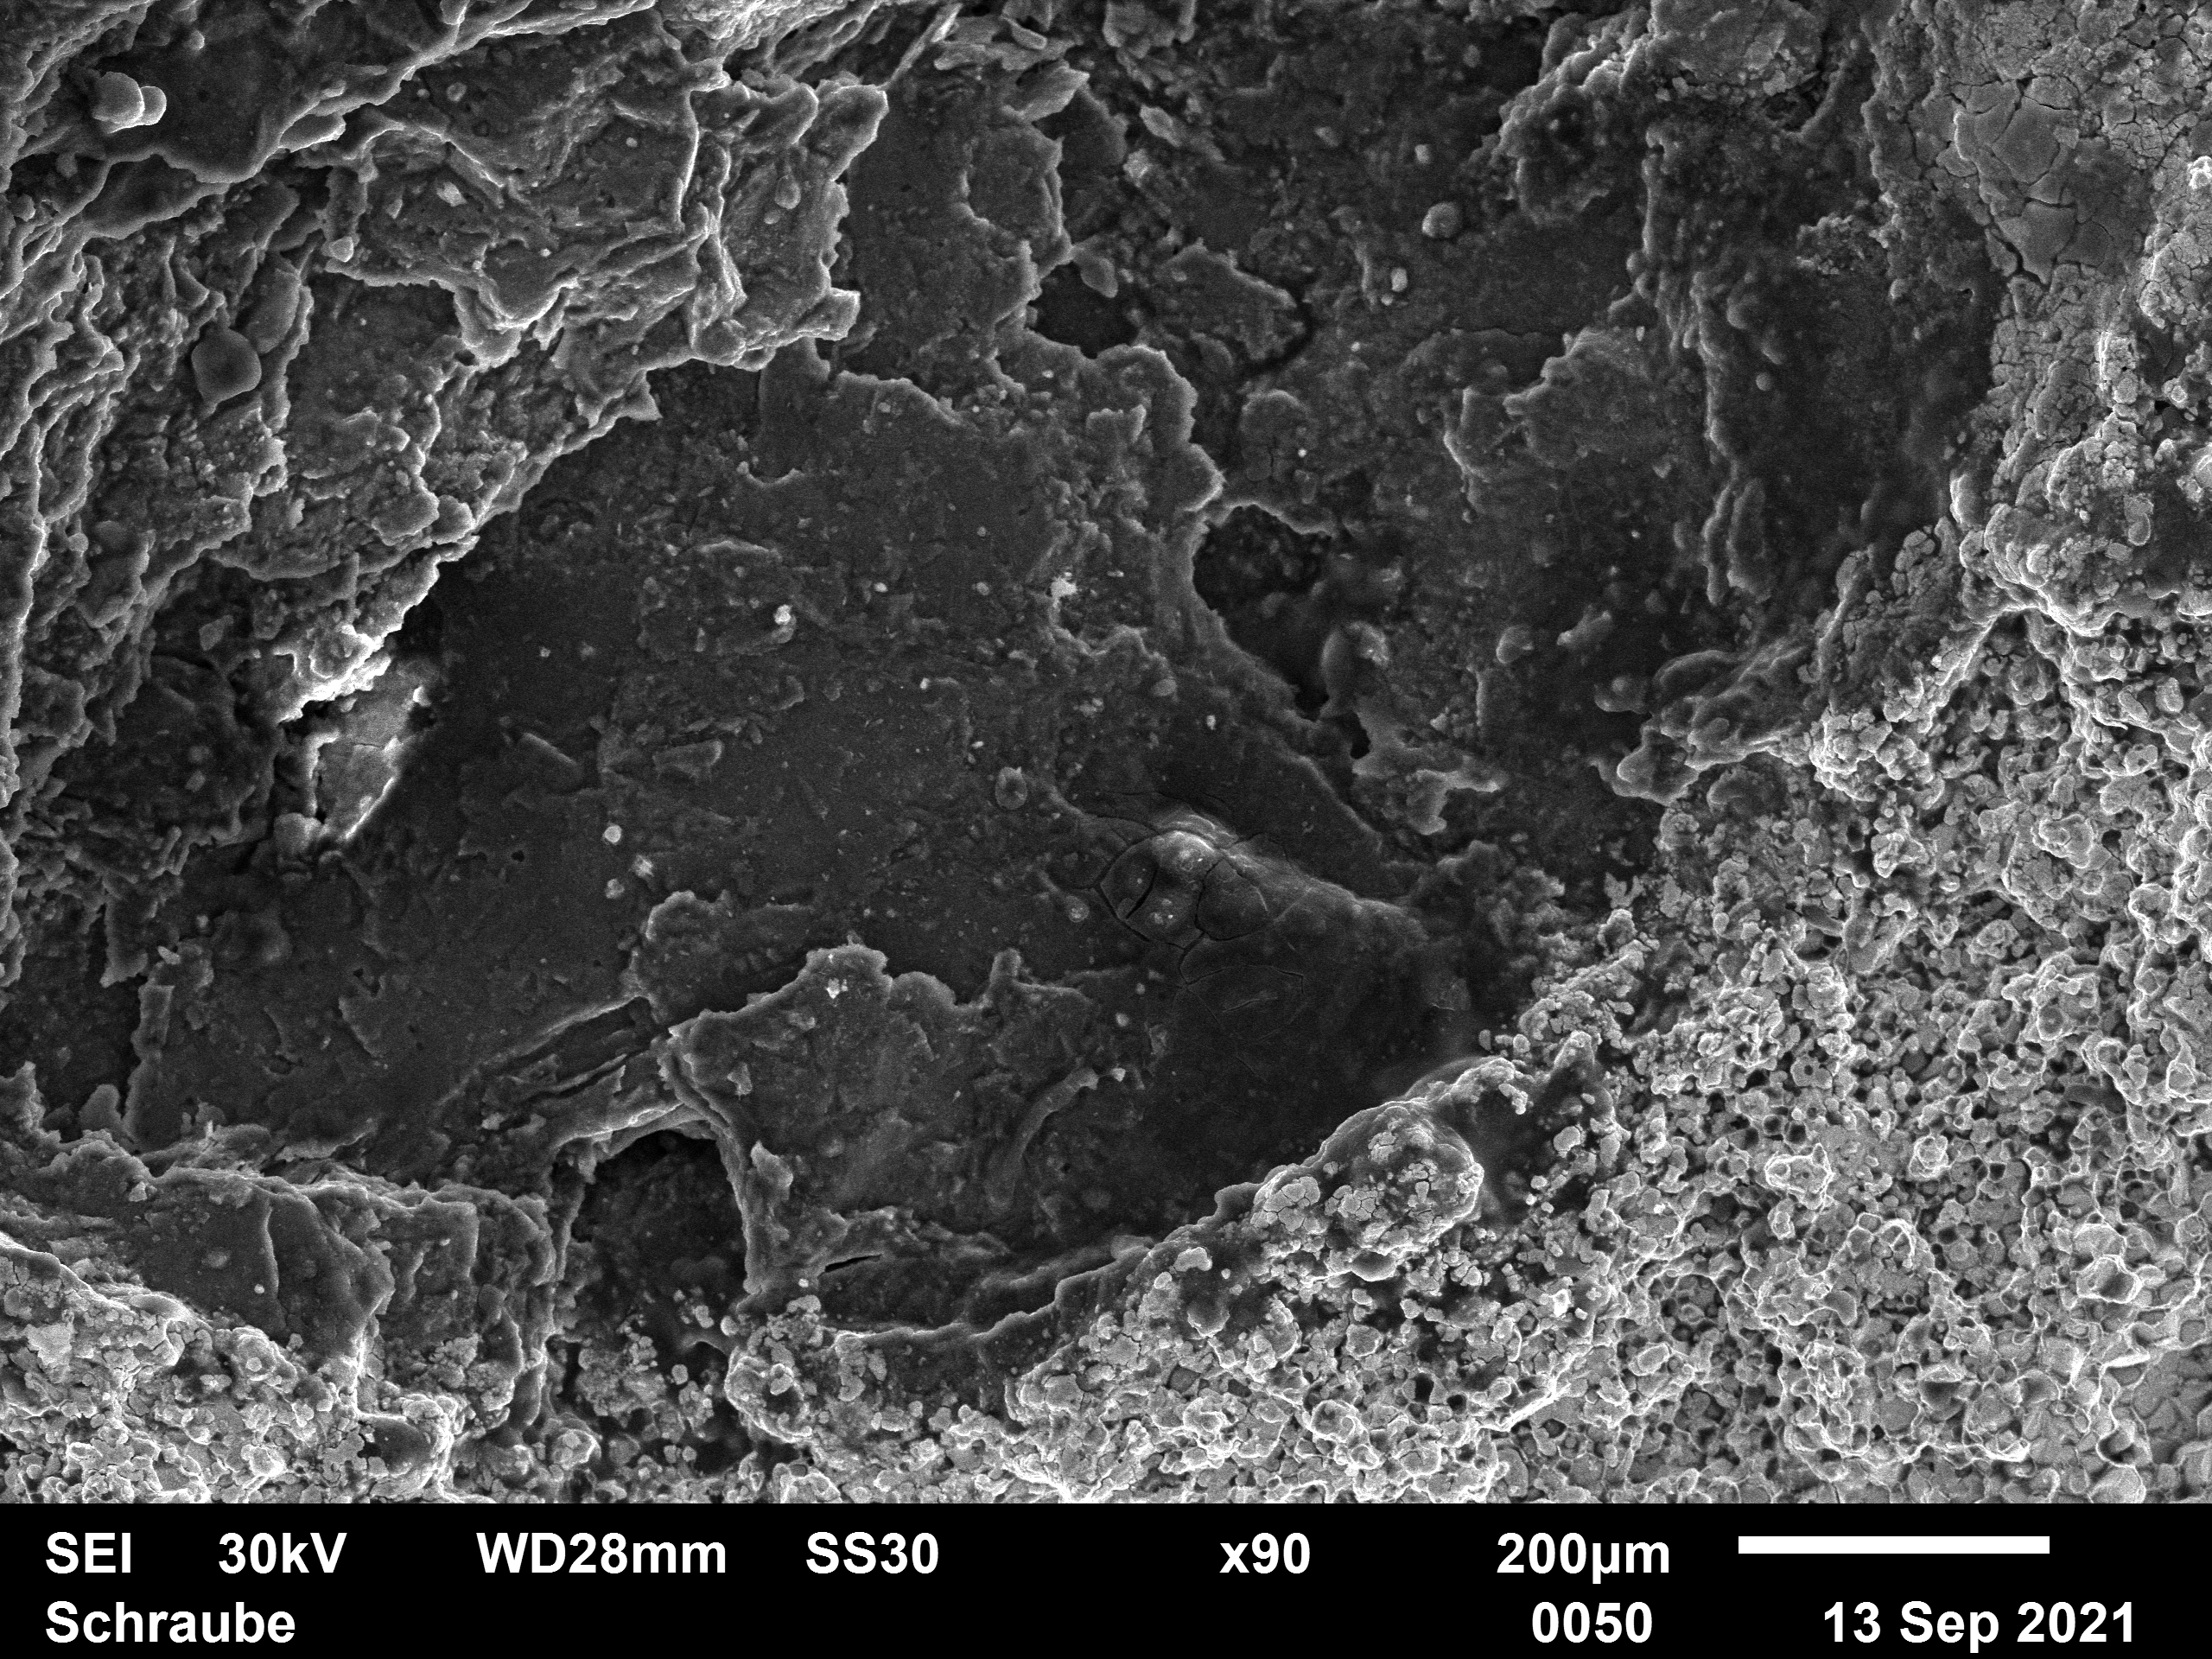
\includegraphics[width=\textwidth]{Auswertung/D/0050.png}
        \caption{SEI}
    \end{subfigure}
    \hfill
    \begin{subfigure}[b]{0.45\textwidth}
        \centering
        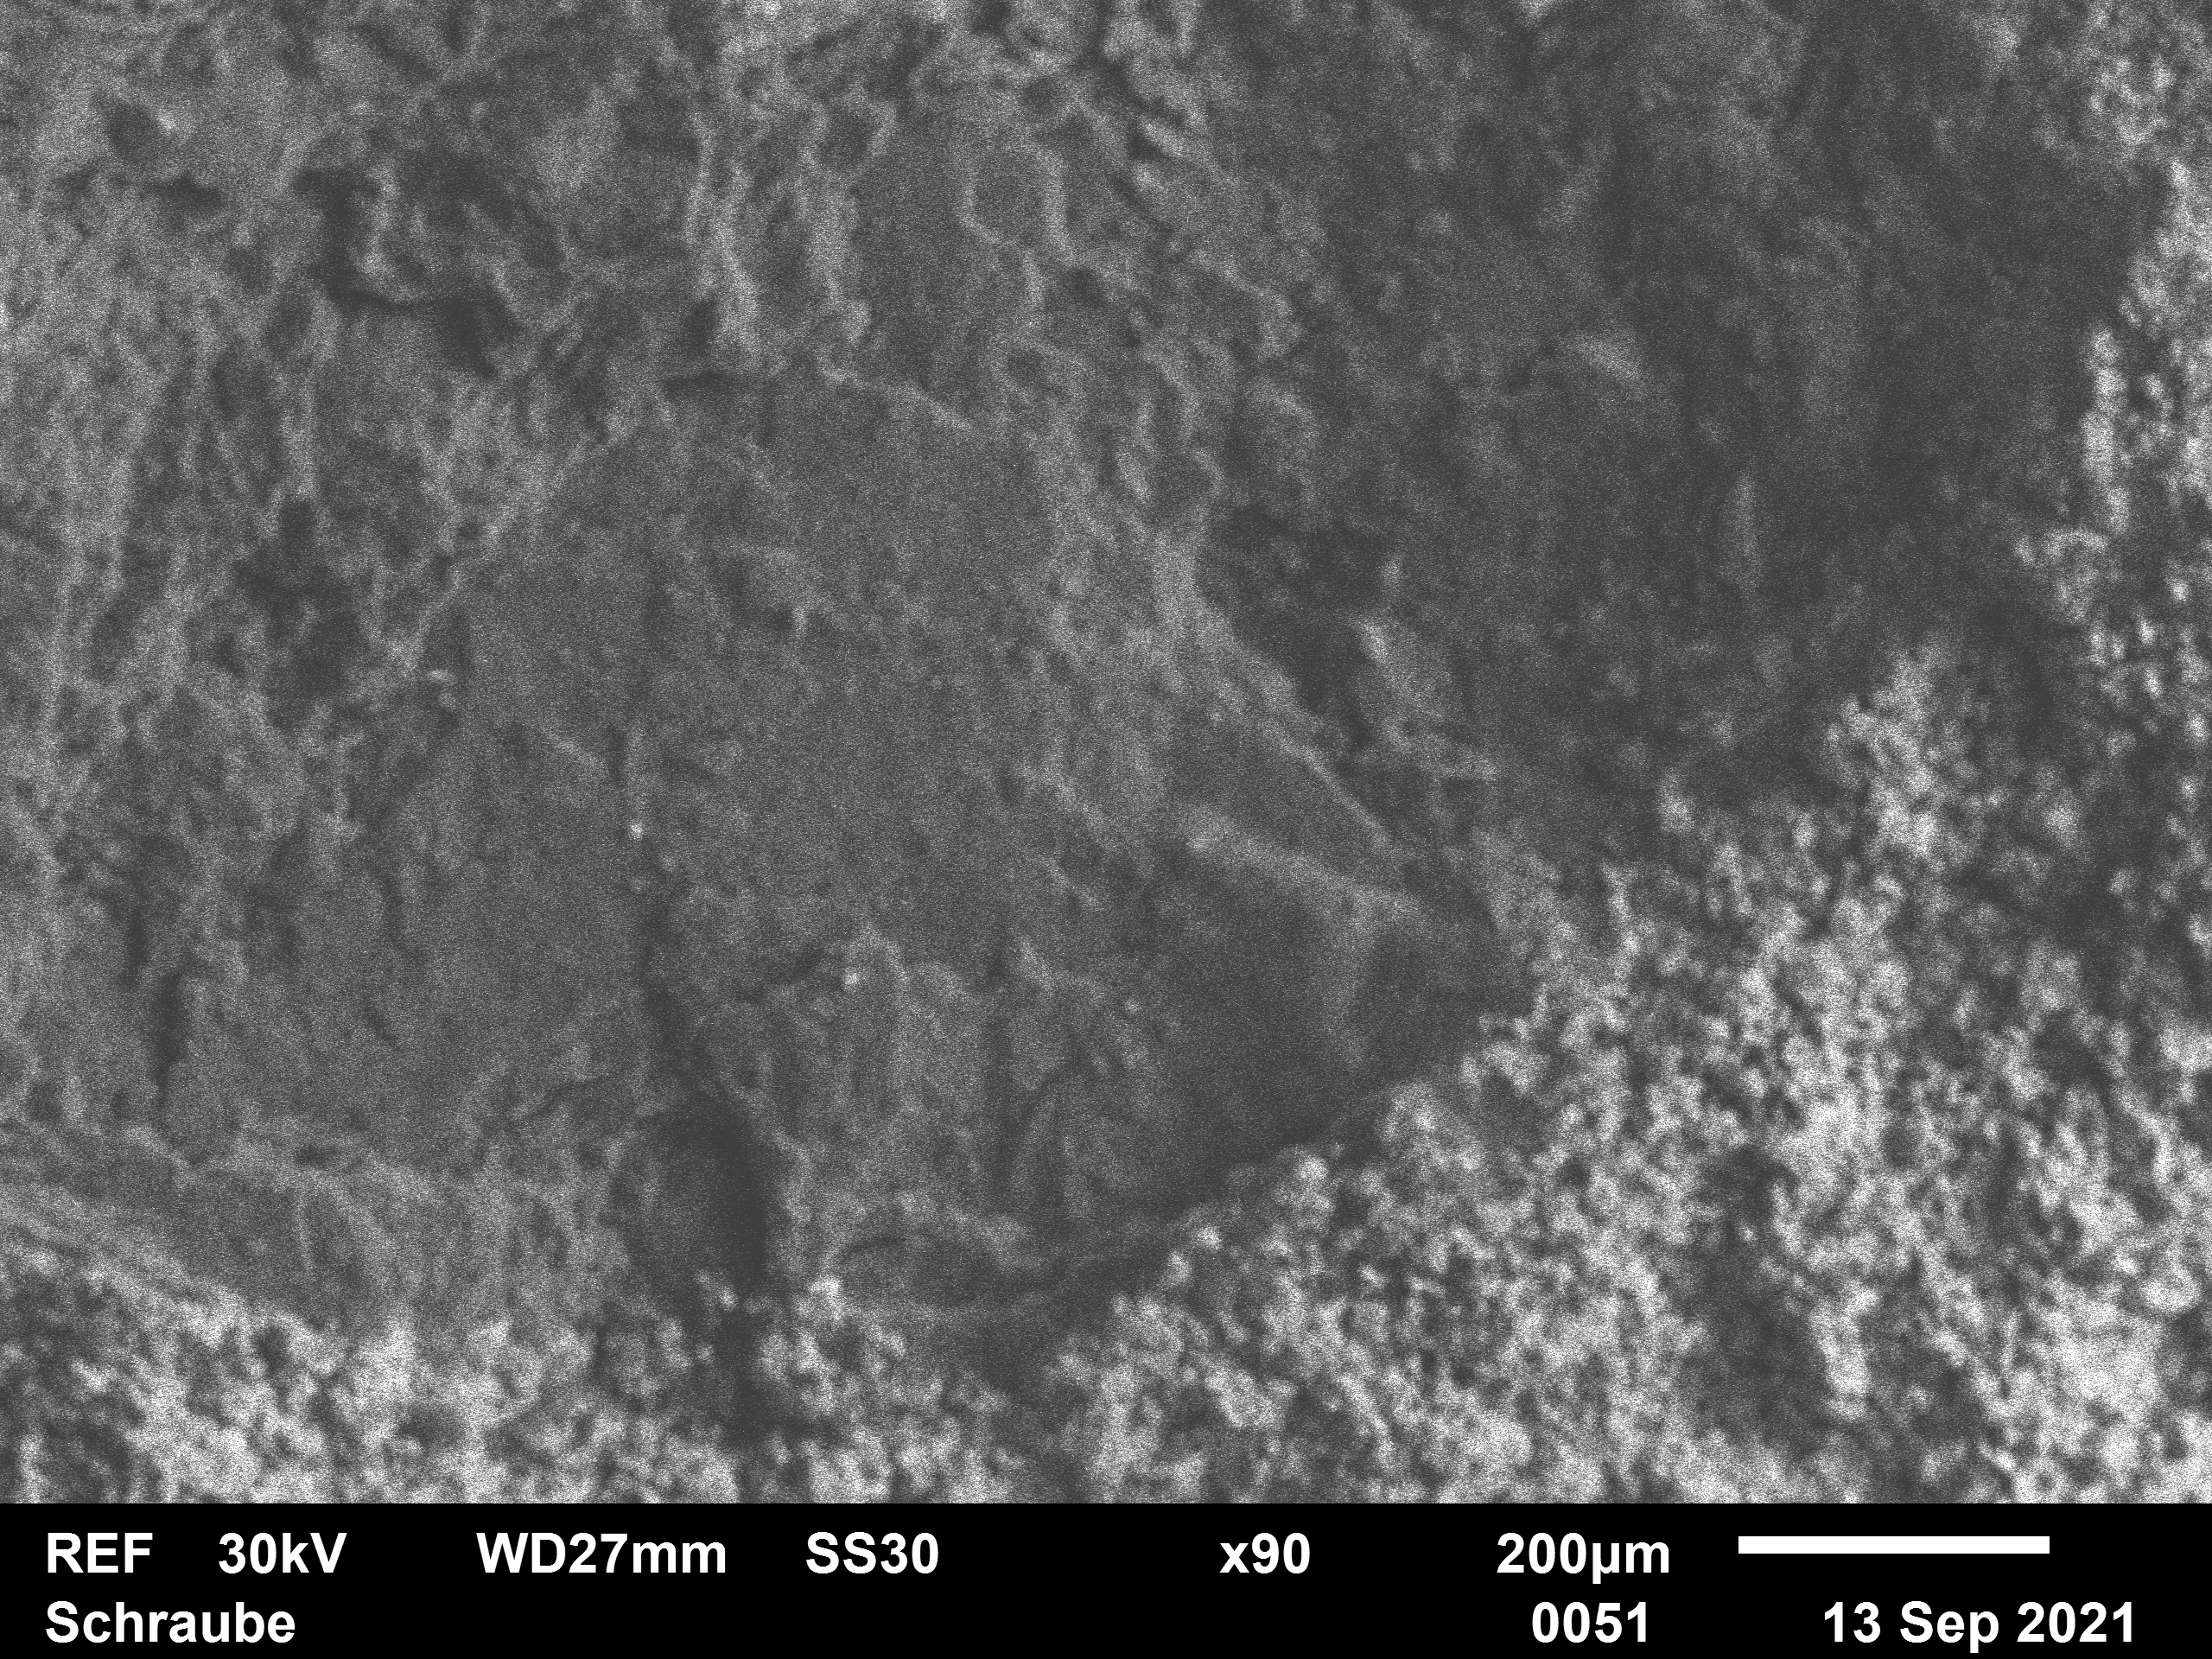
\includegraphics[width=\textwidth]{Auswertung/D/0051.png}
        \caption{REF}
    \end{subfigure}
    \caption{Nahaufnahme der Kante des dunklen Flecks}
\end{figure}

Aus diesen Aufnahmen geht hervor, dass der dunkle Fleck mit einer Vertiefung einhergeht, was durch den Schatten im REF Bild zu erkennen ist. Außerdem unterscheidet sich die Textur deutlich. Im dunklen Bereich gibt es mehr ebene Flächen, wohingegen der hellere Bereich deutlich rauer ist. Das lässt darauf schließen, dass sich im dunklen Bereich eine Verunreinigung evtl. ein Fremdpartikel befand.

\newpage
Nun soll eine EDX Analyse über die Materialzusammensetzung des dunklen Flecks Aufschluss geben.
\begin{figure}[h]
    \centering
    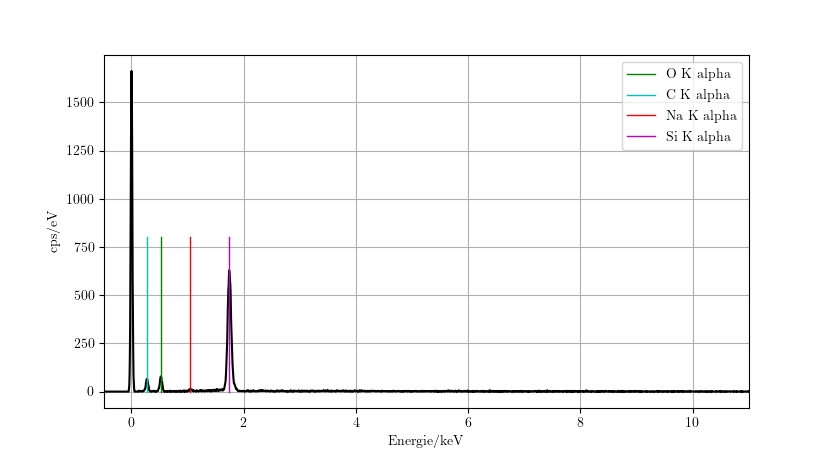
\includegraphics[width=\textwidth]{Auswertung/D/DunkelEDX.png}
    \caption{Röntgenspektrum des dunklen Flecks}
\end{figure}


\begin{table}[h]
    \centering
    \begin{tabular}{c|c|c|c|c|c|c}
        Element & OZ &Serie& unn. C & norm. C &  Atom. C  & Fehler (1 Sigma) \\
         & & & [Gew. \%] & [Gew. \%] & [At. \%] & [Gew. \%] \\
        \hline\hline
        C & 6 & K & 56,69 & 43,02 & 55,43 & 14,77\\
        O & 8 & K & 41,46 & 31,46 & 30,43 & 10,20\\
        Na & 11 & K & 0,89 & 0,67 & 0,45 & 0,16\\
        Si & 14 & K & 32,74 & 24,85 & 13,69 & 1,56
    \end{tabular}
    \caption{Ergebnisse der EDX-Analyse des dunklen Bereichs}
\end{table}
Es fällt auf, dass kein Metall, welches in Schrauben üblicherweise verwendet wird, gefunden wurde. Dies bekräftigt die Theorie, nach welche der dunkle Fleck durch eine Verunreinigung entstanden ist.

\newpage
Des Weiteren zeigt eine Nahaufnahme der hellen Gegenden, dass sich diese durch eine gewisse Erhabenheit auszeichnen, was durch die zu erkennende Kante im Bild deutlich wird. Außerdem erscheint die Oberfläche in diesem Bereich ebener.
\begin{figure}[h]
    \centering
    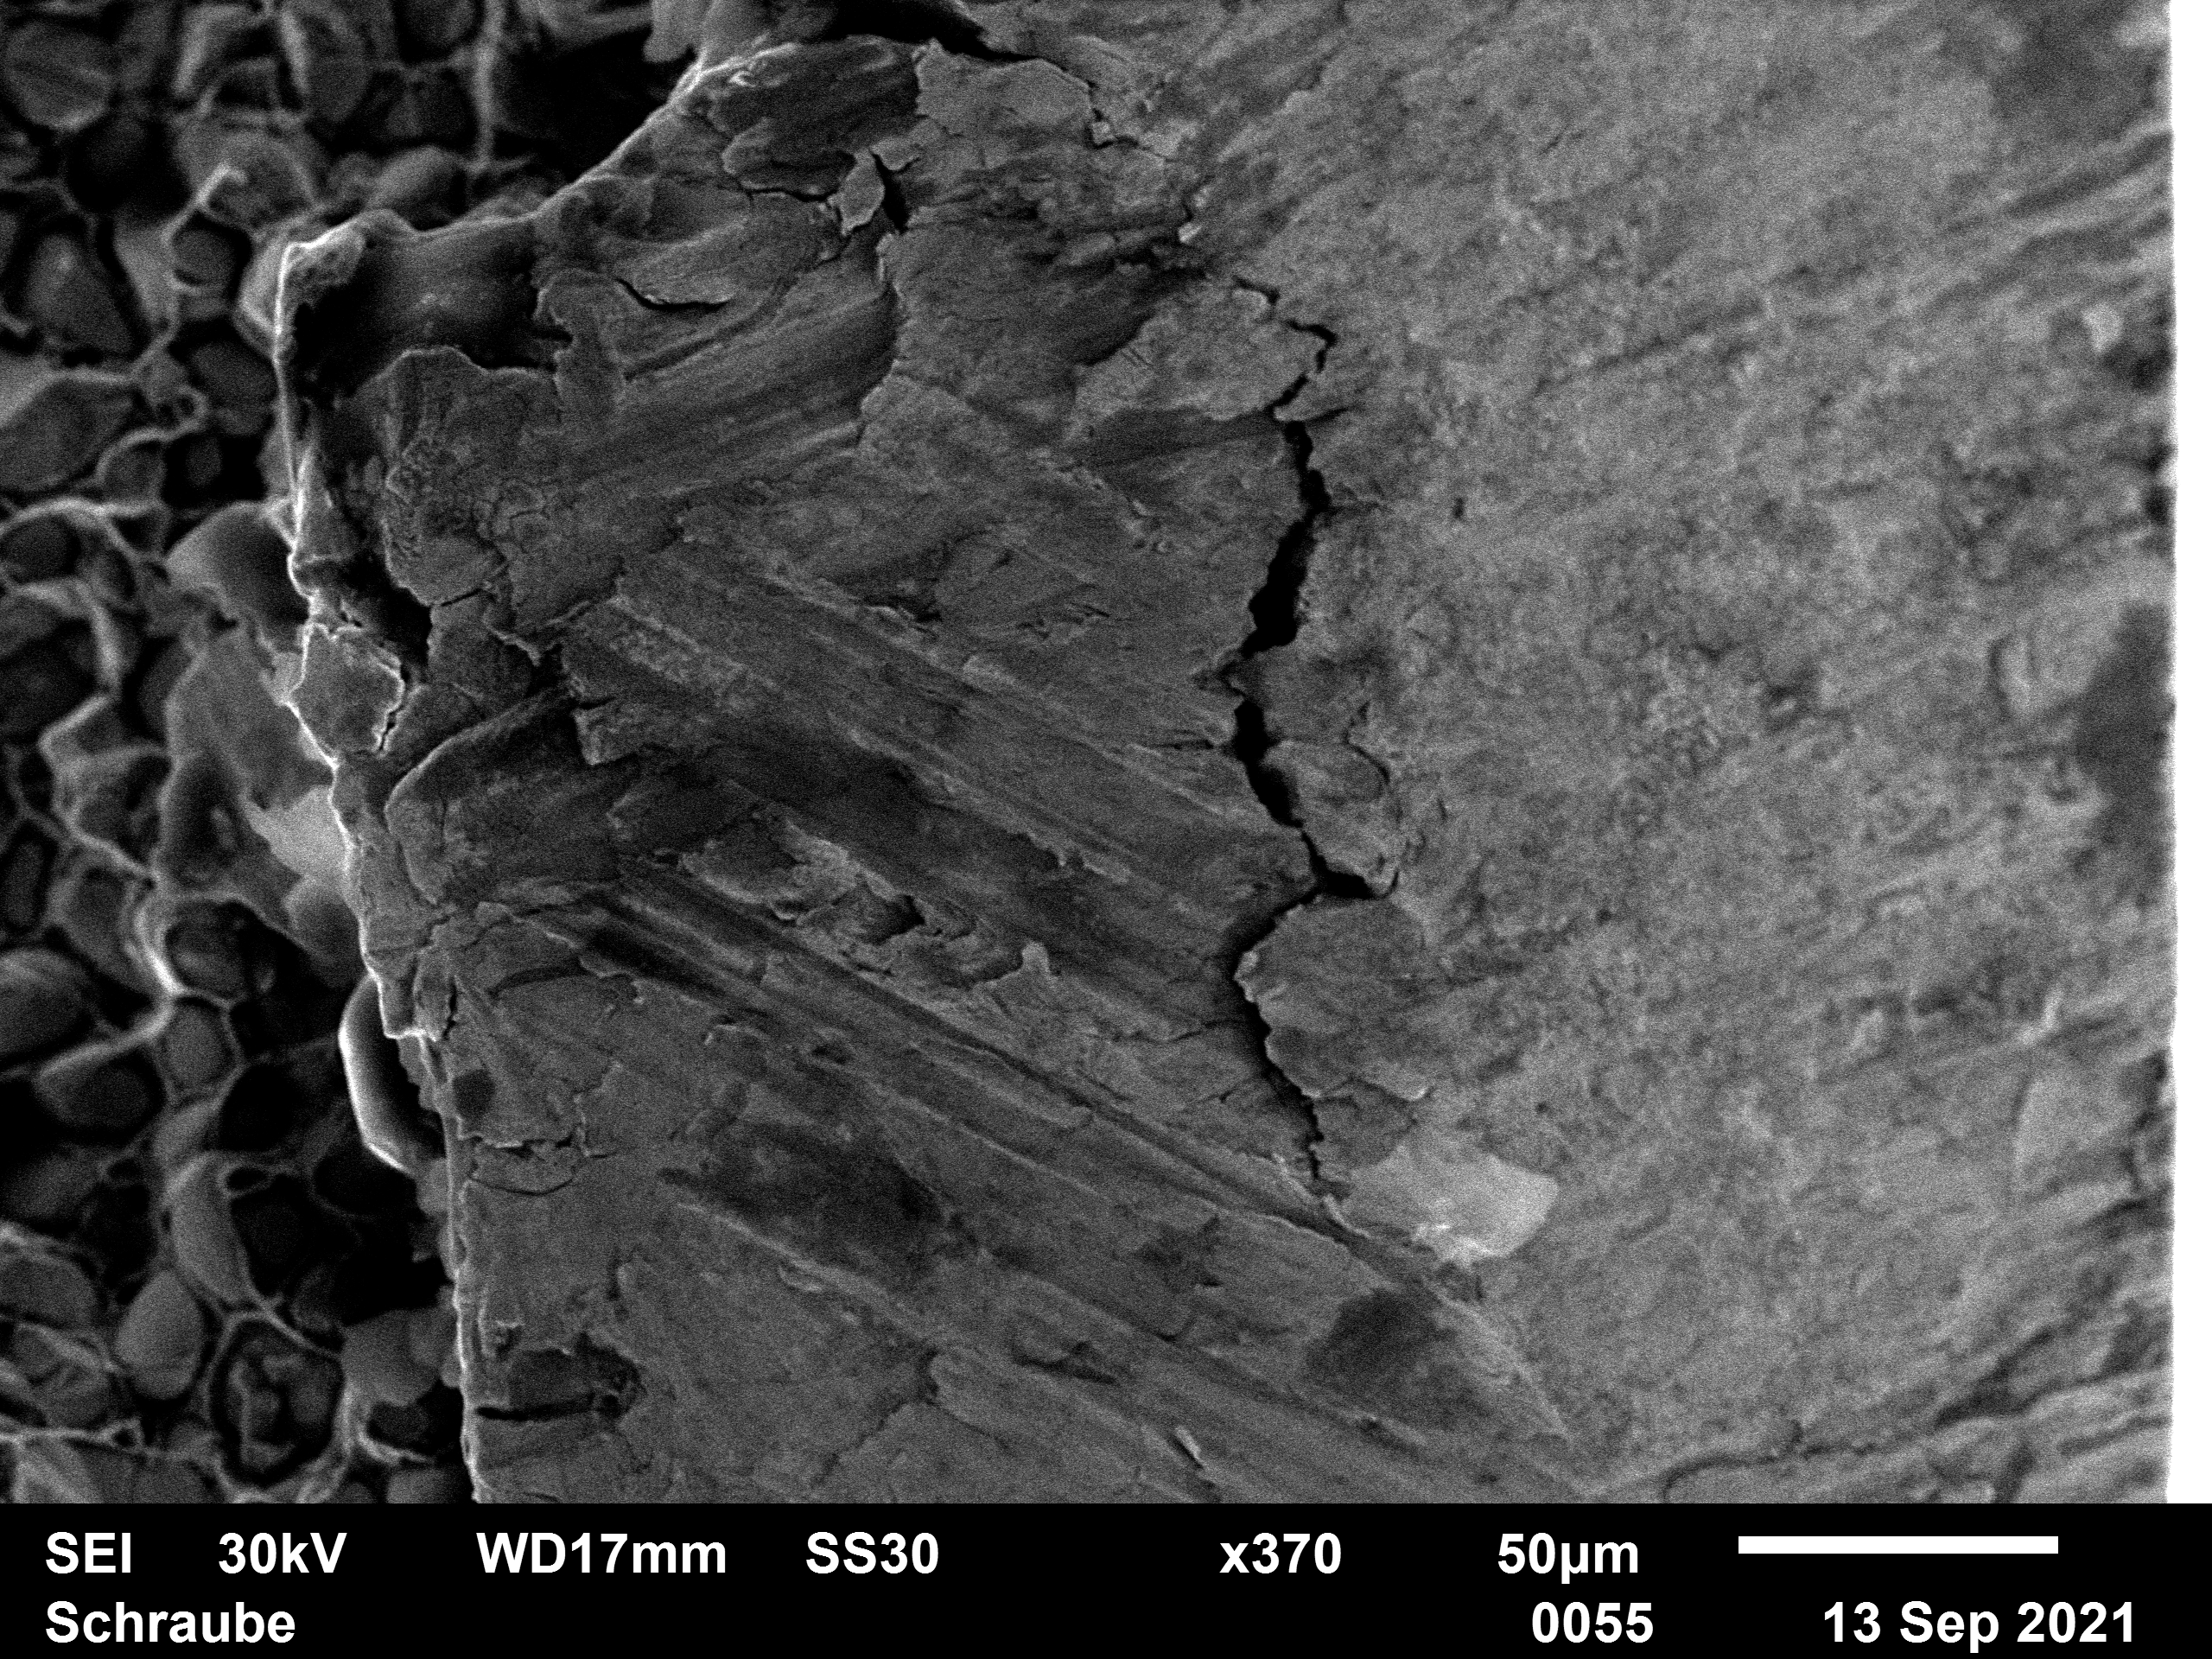
\includegraphics[width=\textwidth]{Auswertung/D/0055.png}
    \caption{Nahaufnahme einer hellen Region}
\end{figure}

\newpage
Über die Zusammensetzung soll wiederum eine EDX Analyse Aufschluss geben.
\begin{figure}[h]
    \centering
    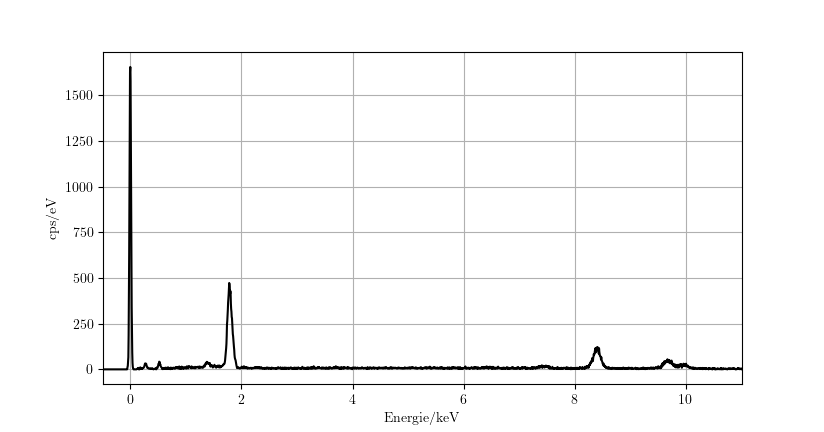
\includegraphics[width=\textwidth]{Auswertung/D/HellEDX.png}
    \caption{Röntgenspektrum der hellen Bereiche}
\end{figure}



\begin{table}[h]
    \centering
    \begin{tabular}{c|c|c|c|c|c|c}
        Element & OZ &Serie& unn. C & norm. C &  Atom. C  & Fehler (1 Sigma) \\
         & & & [Gew. \%] & [Gew. \%] & [At. \%] & [Gew. \%] \\
        \hline\hline
        C & 6 & K & 18,02 & 16,52 & 52,93 & 5,99\\
        O & 8 & K & 14,29 & 13,10 & 31,51 & 4,47\\
        Fe & 26 & K & 0,57 & 0,53 & 0,36 & 0,08\\
        Ni & 28 & K & 1,38 & 1,27 & 0,83 & 0,12\\
        W & 74 & L & 74,81 & 68,59 & 14,36 & 2,09
    \end{tabular}
    \caption{Ergebnisse der EDX-Analyse der hellen Bereiche}
\end{table}
Hier fällt die große Menge an Wolfram und Kohlenstoff auf.

\newpage
Nicht zu vergessen ist das Grundmaterial der Schraube, auch hierbei wird wieder eine EDX Analyse benutzt.
\begin{figure}[h]
    \centering
    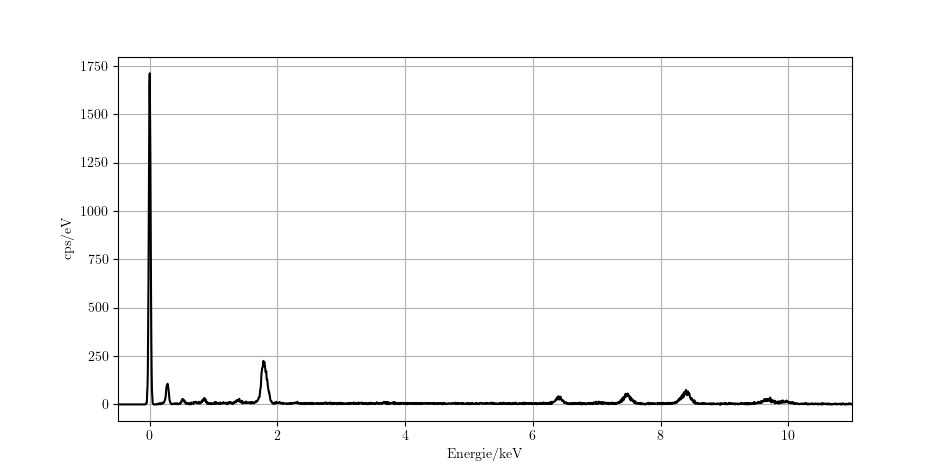
\includegraphics[width=\textwidth]{Auswertung/D/NormalEDX.png}
    \caption{Röntgenspektrum der normalen Bereiche}
\end{figure}


\begin{table}[h]
    \centering
    \begin{tabular}{c|c|c|c|c|c|c}
        Element & OZ &Serie& unn. C & norm. C &  Atom. C  & Fehler (1 Sigma) \\
         & & & [Gew. \%] & [Gew. \%] & [At. \%] & [Gew. \%] \\
        \hline\hline
        C & 6 & K & 42,64 & 43,61 & 78,17 & 9,71\\
        O & 8 & K & 9,86 & 10,08 & 13,57 & 3,42\\
        Fe & 26 & K & 3,94 & 4,03 & 1,55 & 0,20\\
        Ni & 28 & K & 6,88 & 7,04 & 2,58 & 0,28\\
        W & 74 & L & 34,45 & 35,24 & 4,13 & 1,08
    \end{tabular}
    \caption{Ergebnisse der EDX-Analyse der normalen Bereiche}
\end{table}

Unter Berücksichtigung der soeben erlangten Erkenntnisse erscheint es als wahrscheinlich, dass der Dunkle Fleck eine Verunreinigung ist, welche bei der Herstellung in die Schmelze gelang. Diese Vermutung wurde am deutlichsten durch die EDX Analyse bestätigt, da dieser Bereich eine völlig andere Materialzusammensetzung(kaum Metalle; Sondern viel Silizium) besitzt. Die "normalen" und hellen Bereiche setzen sich hingegen aus den gleichen Materialien zusammen. \\

Durch die Verunreinigung (dunkle Anomalie) würde somit die Querschnittsfläche der Legierung an dieser Stelle verkleinert. Dies führte deshalb zu einer verminderung der stabilität, weshalb die Schraube an dieser Stelle gebrochen ist.

\newpage
\section{Chip Wafer}

Im letzten Teil haben wir uns einen Teil eines Chip Wafers vorgenommen.

\begin{figure}[h]
    \centering
    
    \begin{subfigure}[b]{0.45\textwidth}
        \centering
        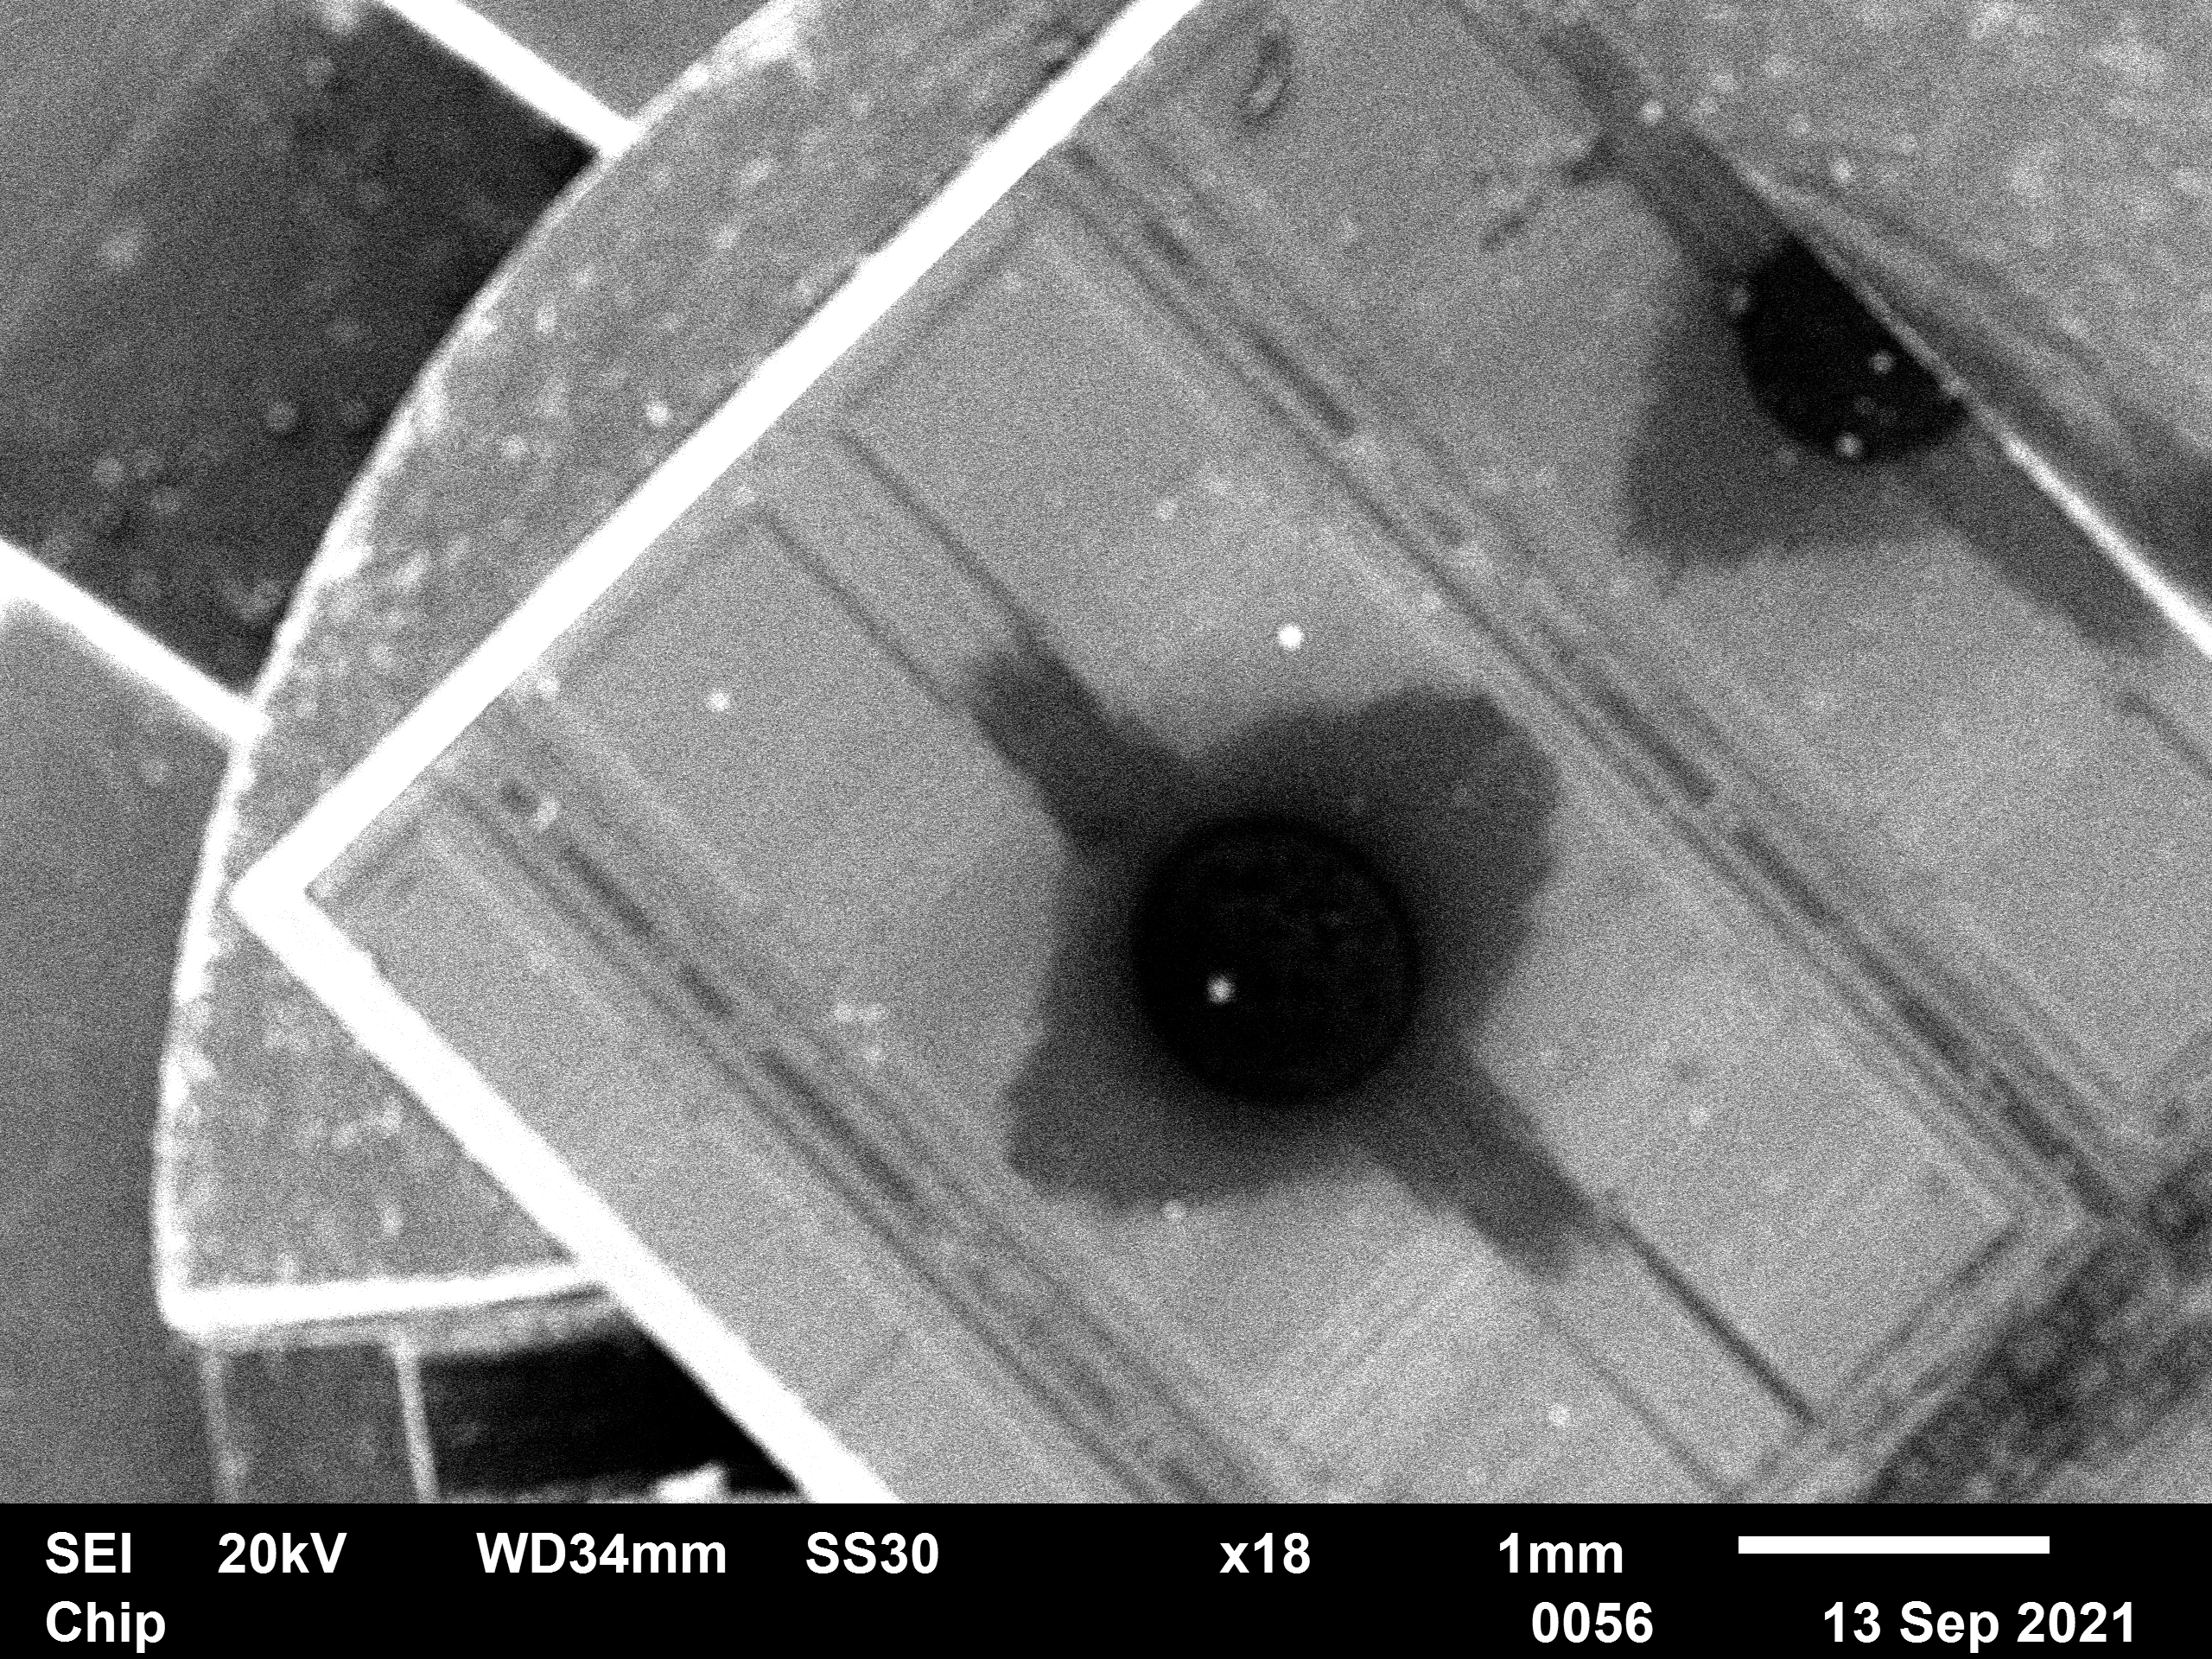
\includegraphics[width=\textwidth]{Auswertung/E/0056.png}
        \caption{Großaufnahme}
    \end{subfigure}
    \hfill
    \begin{subfigure}[b]{0.45\textwidth}
        \centering
        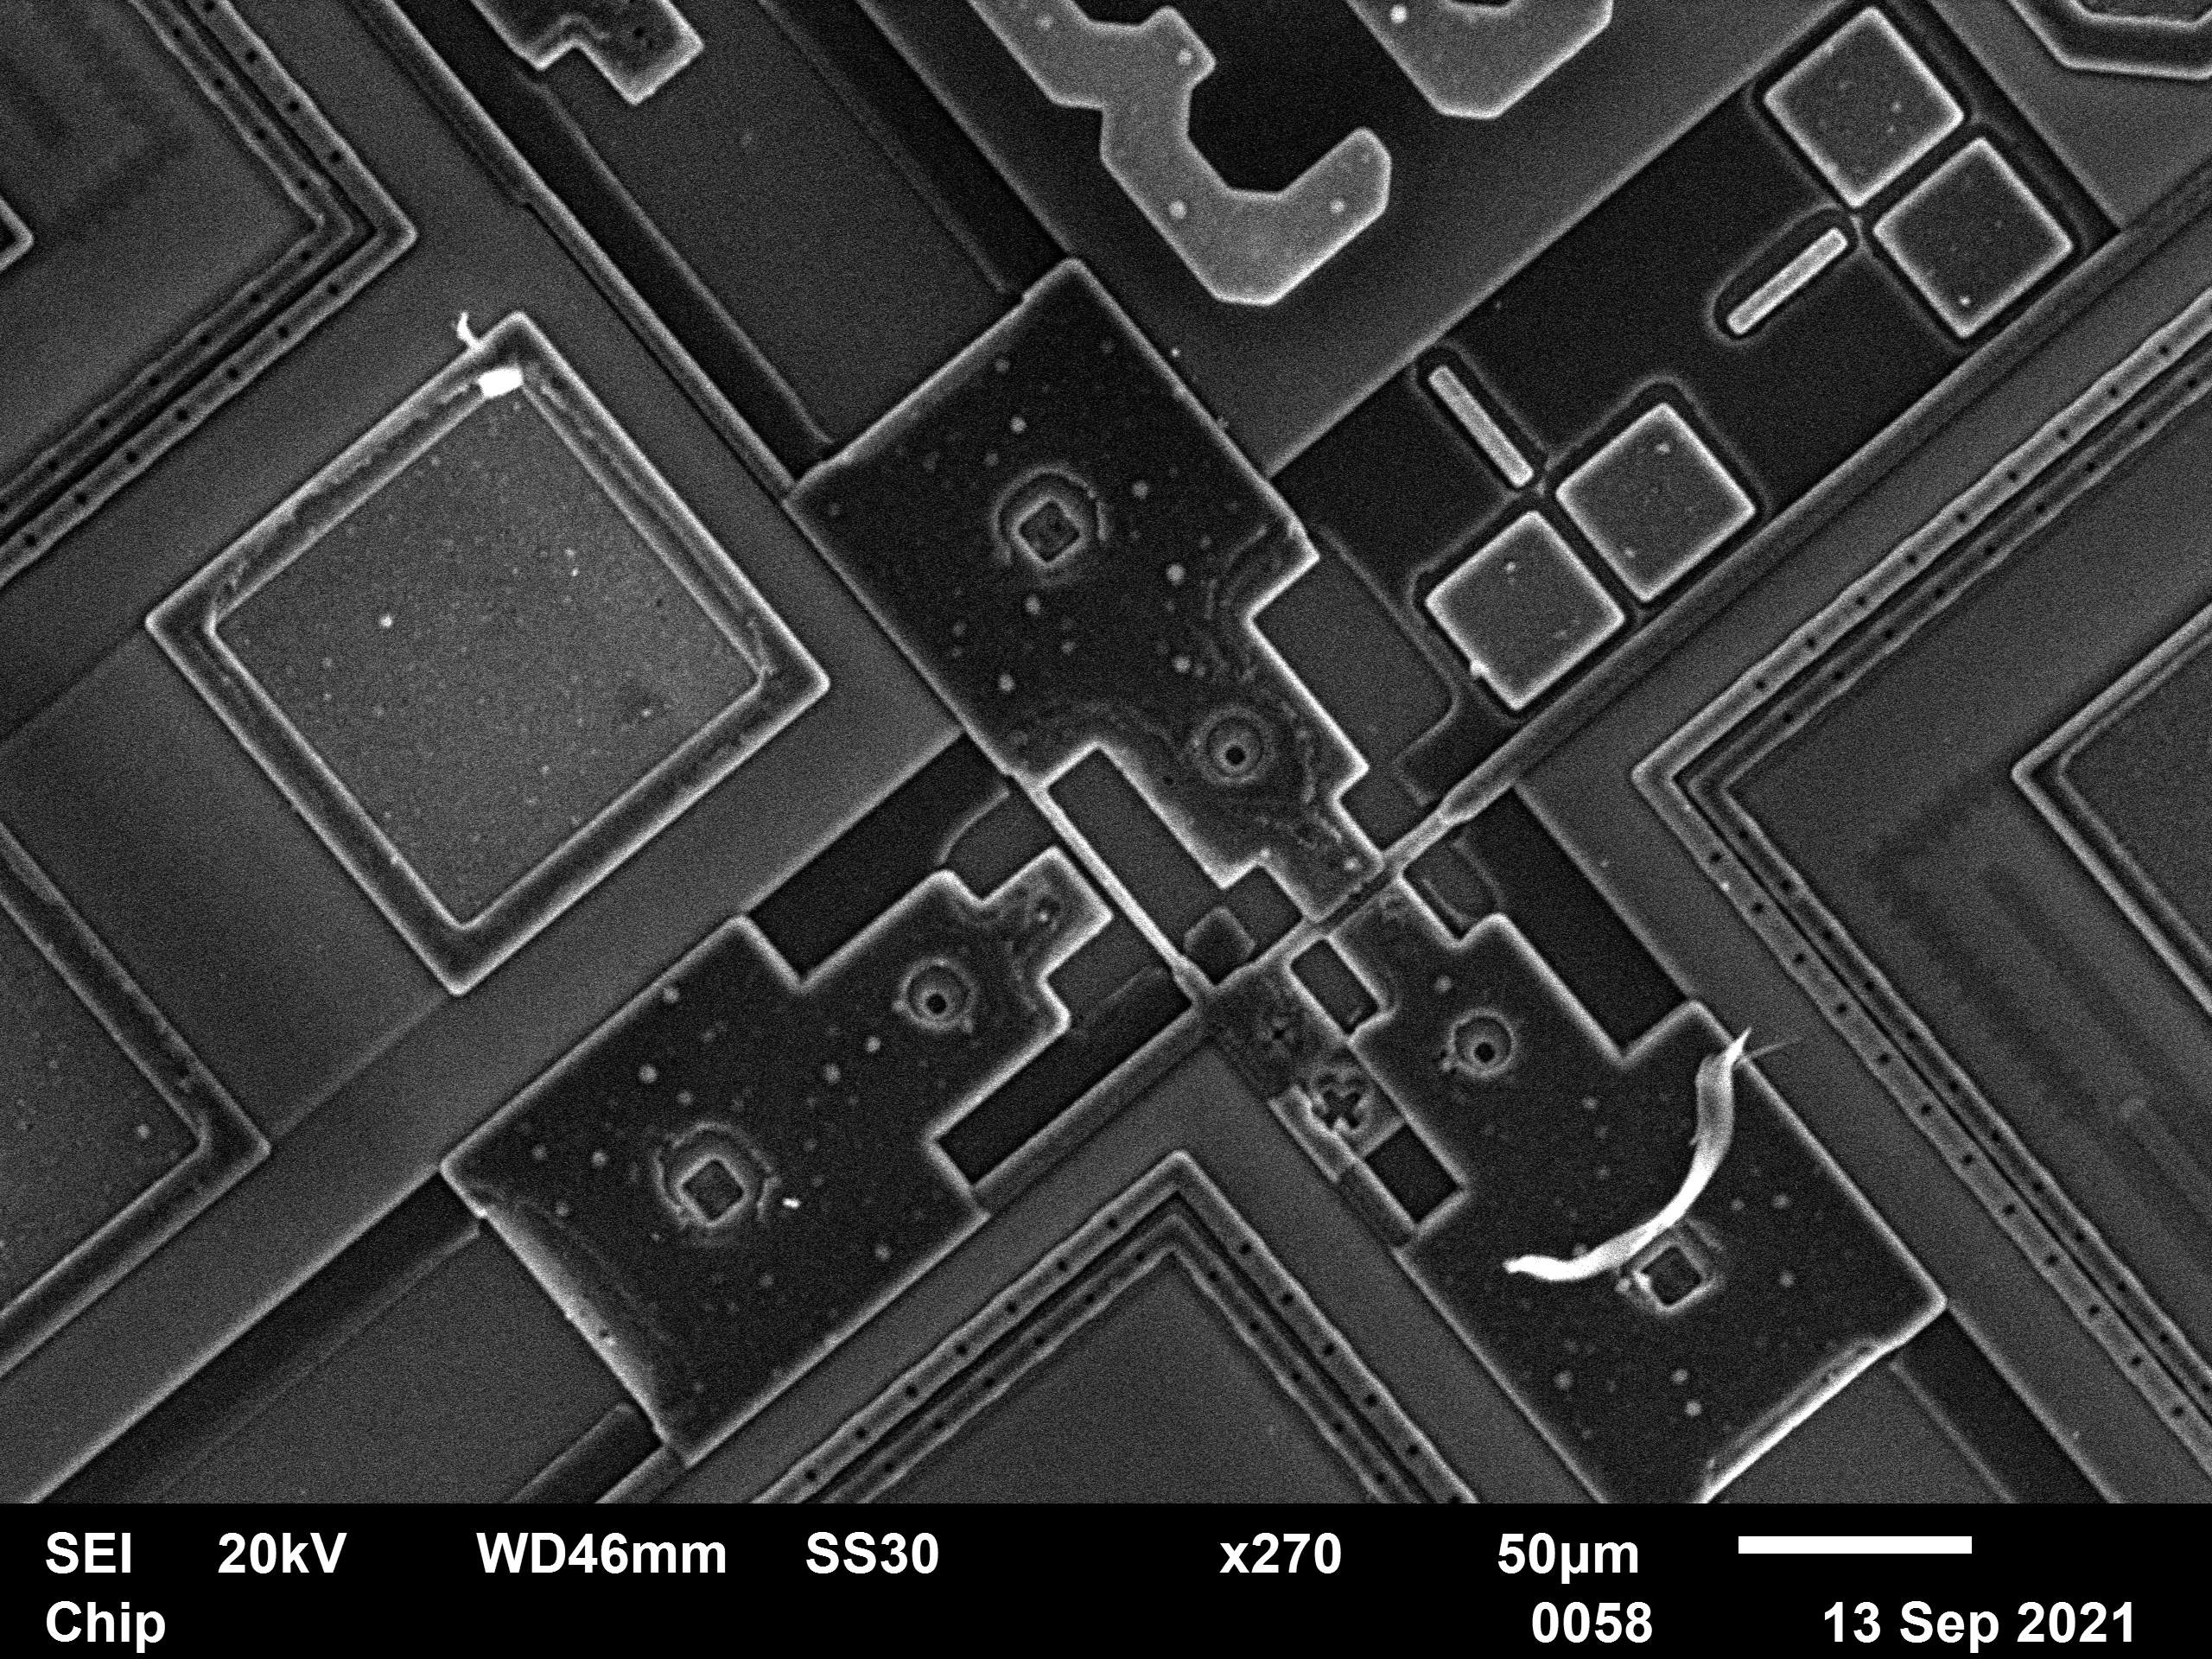
\includegraphics[width=\textwidth]{Auswertung/E/0058.png}
        \caption{Leiterbahnen}
    \end{subfigure}
    \\
    \begin{subfigure}[b]{0.45\textwidth}
        \centering
        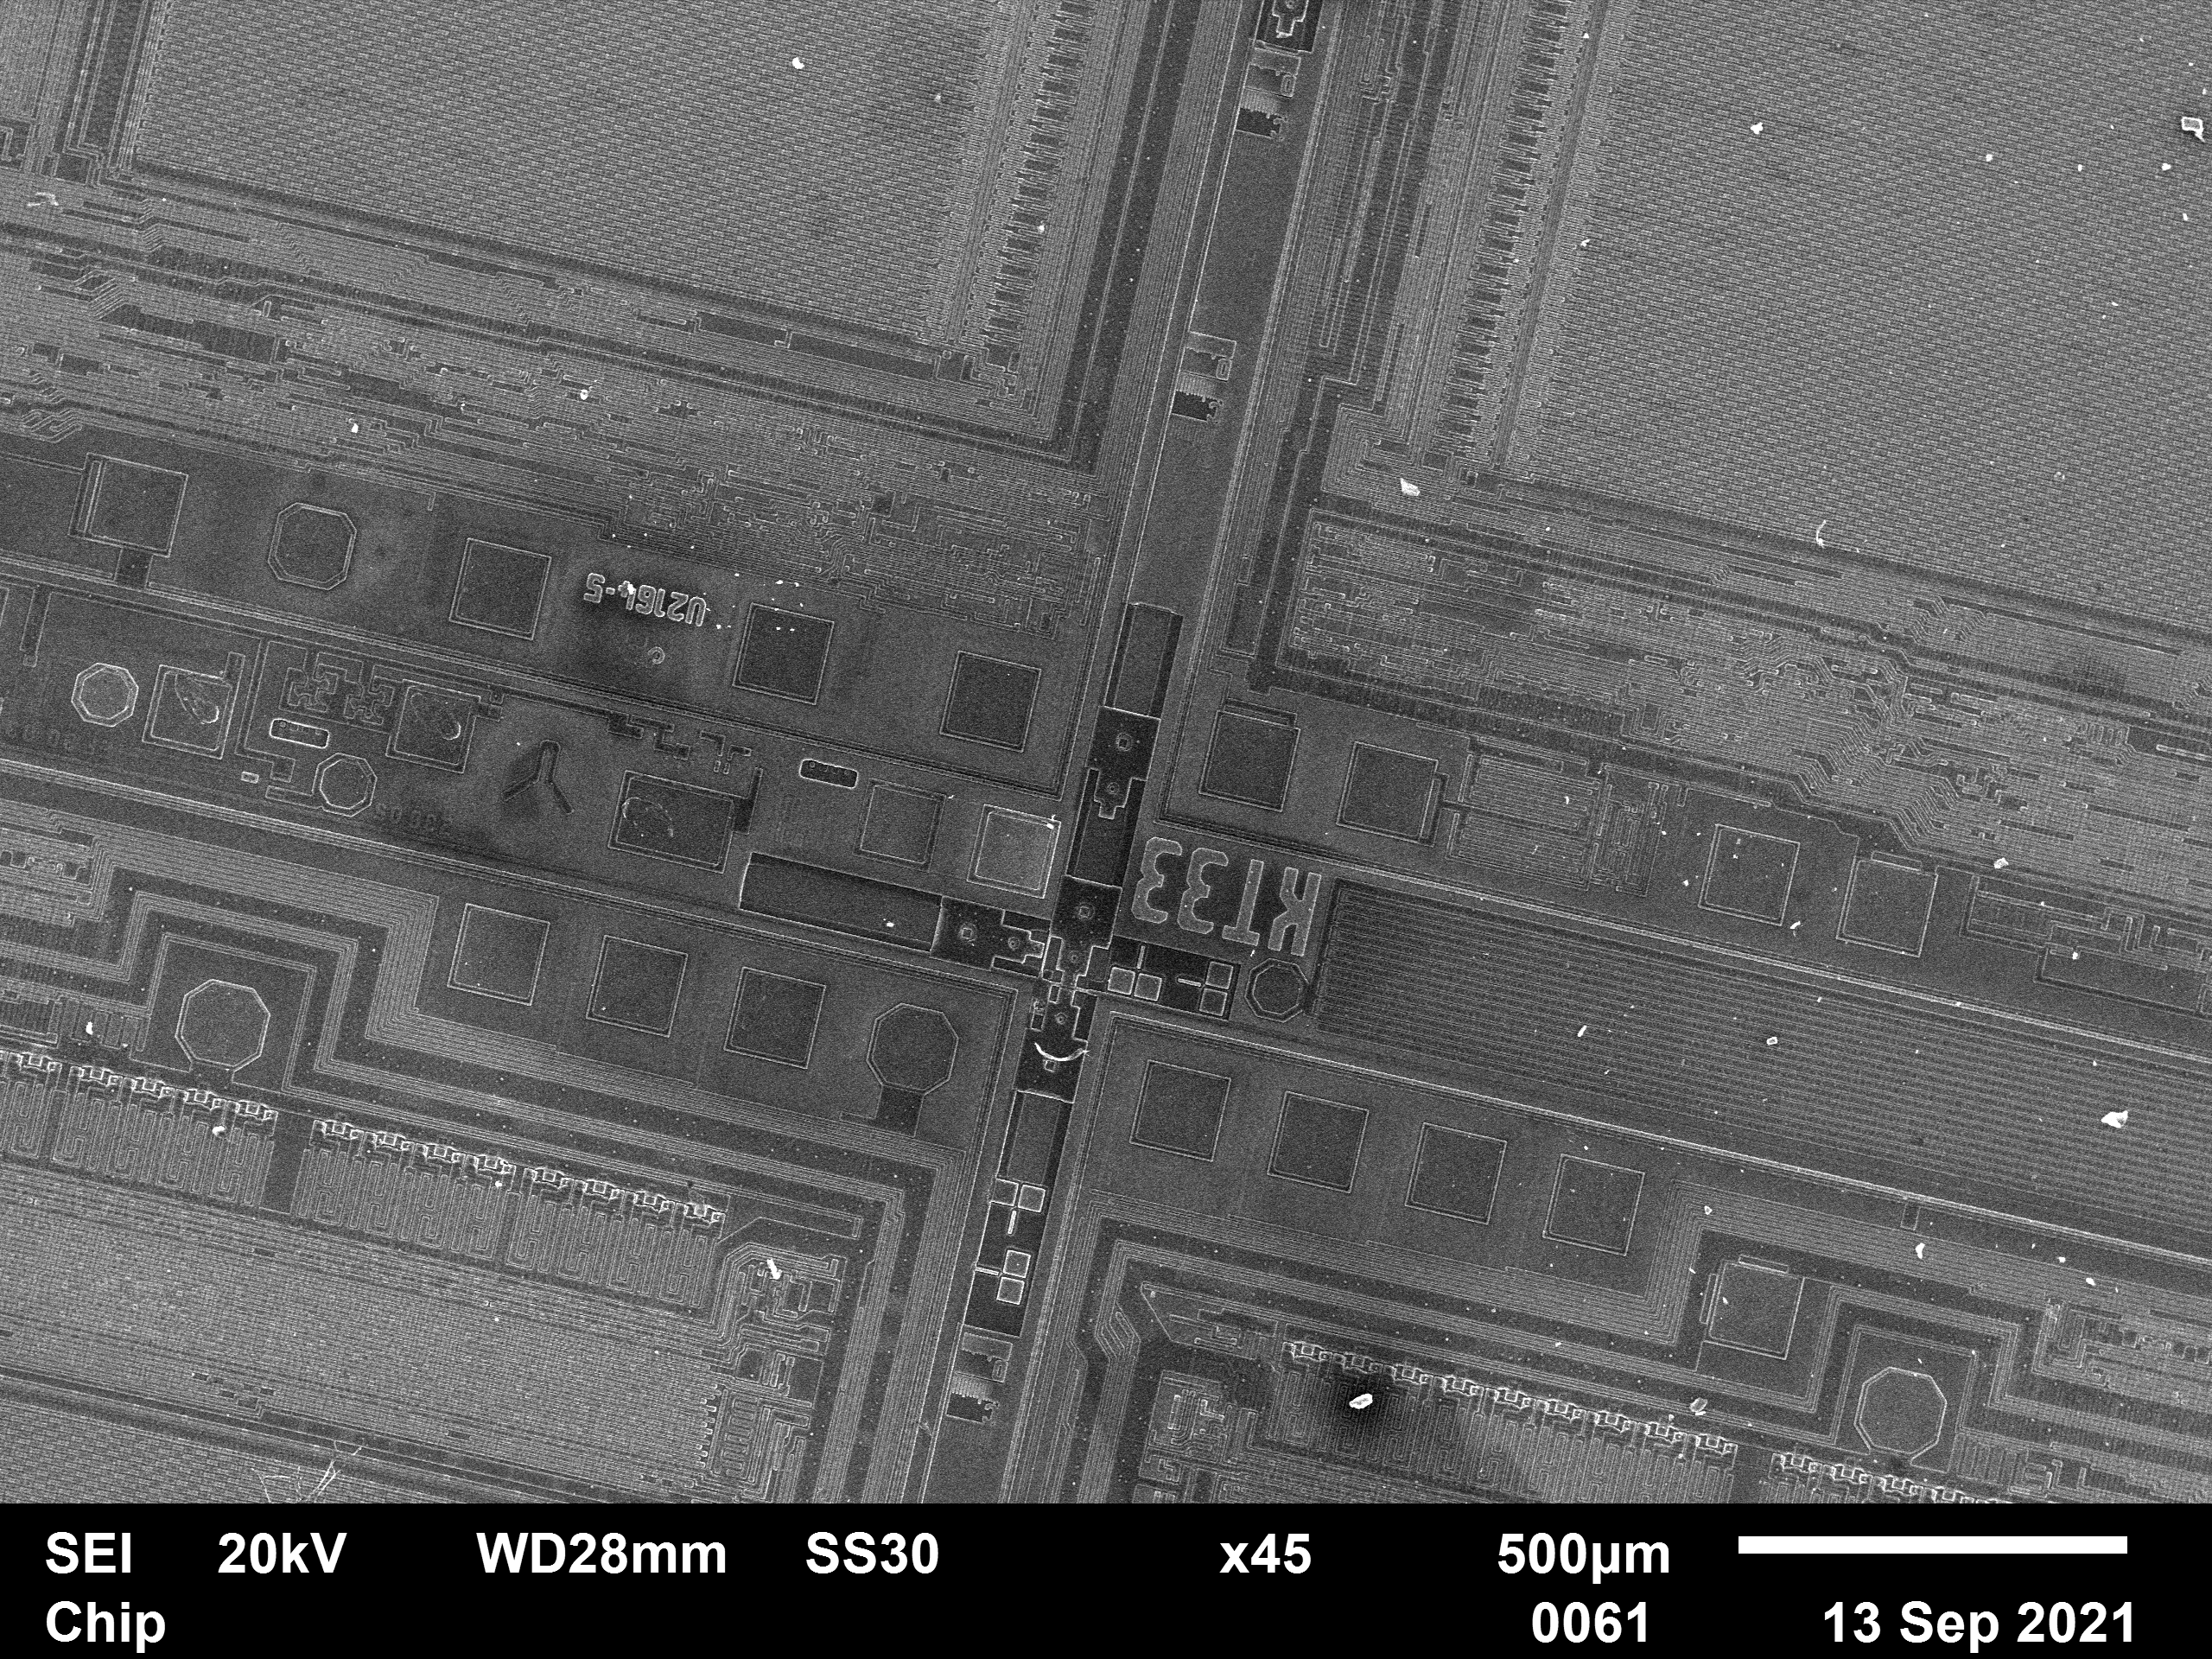
\includegraphics[width=\textwidth]{Auswertung/E/0061.png}
        \caption{Leiterbahnen}
    \end{subfigure}
    \hfill
    \begin{subfigure}[b]{0.45\textwidth}
        \centering
        \includegraphics[width=\textwidth]{Auswertung/E/0063.png}
        \caption{Logo}
    \end{subfigure}
    \caption{Bilder des Wafers}
\end{figure}
Gut zu erkennen sind die Leiterbahnen. Außerdem konnten wir auch ein Logo finden, wir vermuten es soll ein Mammut darstellen.